\documentclass[french, 12pt]{report}

%-------------------------------------------------------------------------------
\usepackage[a4paper,top=2cm,bottom=2cm,left=2cm,right=2cm,marginparwidth=1.75cm]{geometry}
\usepackage{amsmath,amsfonts,amssymb,amsthm}
\usepackage[french]{babel}
\usepackage[utf8]{inputenc}
\usepackage[T1]{fontenc}
\usepackage{enumerate}
\usepackage{natbib}
\usepackage{graphicx}
\usepackage{xspace}
\usepackage{color,xcolor}
\usepackage{tikz}
\usepackage{remreset}
\usepackage{url}
\usepackage{arydshln}
\usepackage{boites}
\usepackage{fontawesome}

% \usepackage{extsizes} % Permet \documentclass[french, 14pt]{extreport}
% \usepackage[a4paper,top=1cm,bottom=2cm,left=1cm,right=1cm,marginparwidth=.75cm]{geometry}
\usepackage{minitoc}

\graphicspath{{../Figures/}}
% Environnement
\newtheorem{theorem}{Théorème}
\newtheorem{definition}{Définition}
\newtheorem{lemma}{Lemme}
\newtheorem{proposition}{Proposition}
\newtheorem*{theorem*}{Théorème}
\newtheorem*{definition*}{Définition}
\newtheorem*{proposition*}{Proposition}
\newtheorem*{corollary*}{Corollaire}
\newtheorem*{assumption*}{Hypothèse}
\newtheorem*{algorithm*}{Algorithme}
\newtheorem*{lemma*}{Lemme}
\newtheorem*{remark*}{Remarque}
\newtheorem*{exercise*}{Exercice}
\newtheorem{exercise}{Exercice}
\newcommand{\remark}{\bigskip\noindent\textbf{\textsl{Remarque.}}\xspace}
\newcommand{\remarks}{\bigskip\noindent\textbf{\textsl{Remarques.}}\xspace}
\newcommand{\parSR}[1]{\paragraph*{\textsl{#1}}\xspace}
\renewcommand{\proof}{\bigskip\noindent\underline{\textsl{Démonstration}.}\xspace}
\newcommand{\eproof}{$\blacksquare$}

% Effets, couleurs
\newcommand{\emphase}[1]{\textcolor{red}{#1}}
\newcommand{\demoProp}[1]{\noindent{\textbf{\textsl{Démonstration de la proposition \ref{#1} :}}}}
\newcommand{\itemdot}{\textbullet}

% Moments
\DeclareMathOperator{\Esp}{\mathbb{E}}
\DeclareMathOperator{\diag}{diag}
\DeclareMathOperator{\Cov}{\mathbb{C}ov}
\DeclareMathOperator{\tr}{tr}
\DeclareMathOperator{\Var}{\mathbb{V}}
\let\Pr\relax\DeclareMathOperator{\Pr}{\mathbb{P}}
\renewcommand{\d}{\text{d}}

% R, N, ...
\newcommand{\cst}{\text{cst}}
\newcommand{\Cbb}{\mathbb{C}}
\newcommand{\Ibb}{\mathbb{I}}
\newcommand{\Nbb}{\mathbb{N}}
\newcommand{\Rbb}{\mathbb{R}}
\newcommand{\Zbb}{\mathbb{Z}}

% Indicateurs

% Lois et ensembles
\newcommand{\Acal}{\mathcal{A}}
\newcommand{\Bcal}{\mathcal{B}}
\newcommand{\Ccal}{\mathcal{C}}
\newcommand{\Ecal}{\mathcal{E}}
\newcommand{\Gcal}{\mathcal{G}}
\newcommand{\Ical}{\mathcal{I}}
\newcommand{\Lcal}{\mathcal{L}}
\newcommand{\Mcal}{\mathcal{M}}
\newcommand{\Ncal}{\mathcal{N}}
\newcommand{\Pcal}{\mathcal{P}}
\newcommand{\Rcal}{\mathcal{R}}
\newcommand{\Scal}{\mathcal{S}}
\newcommand{\Ucal}{\mathcal{U}}
\newcommand{\Xcal}{\mathcal{X}}
\newcommand{\Ycal}{\mathcal{Y}}

% Comments
\newcommand{\SR}[2]{\textcolor{gray}{#1}\textcolor{red}{#2}}
\newcommand{\todo}[1]{\textcolor{red}{\`A faire~: {\sl #1}}}
\newcommand{\dessin}[1]{
\begin{center}\framebox{\begin{minipage}{\textwidth}
  \textcolor{purple}{#1}
\end{minipage}}\end{center}
\bigskip
}
\newcommand{\progres}[1]{
\begin{center}\framebox{\begin{minipage}{\textwidth}
  \textcolor{blue}{{\sl #1}}
\end{minipage}}\end{center}
\bigskip
}
\newcommand{\solution}[1]{
\begin{center}\framebox{\begin{minipage}{\textwidth}
  \noindent{\sl Solution :}
  #1
\end{minipage}}\end{center}
\bigskip
}
% \newcommand{\exemple}[1]{
% \begin{center}\framebox{\begin{minipage}{\textwidth}
%   \parSR{Exemple.}
%   #1
% \end{minipage}}\end{center}
% \bigskip
% }
\newcommand{\exemple}[1]{
\begin{breakbox}
  \parSR{Exemple.}
  #1
\end{breakbox}
\bigskip
}

\newcommand{\SRcorrect}[2]{\textcolor{gray}{#1}\textcolor{blue}{#2}}
\newcommand{\SRcomment}[1]{\textcolor{blue}{[{\sl SR: #1}]}}



% Section numbering
\usepackage{chngcntr}
\renewcommand{\thepart}{\Roman{part}}
% \counterwithout{section}{part}
\setcounter{secnumdepth}{4}
\setcounter{tocdepth}{6}

% Proposition numbering
% \numberwithin{theorem}{chapter}
% \numberwithin{lemma}{chapter}
% \numberwithin{proposition}{chapter}
% \numberwithin{exercise}{chapter}
% \numberwithin{definition}{chapter}
% \numberwithin{equation}{chapter}

%-------------------------------------------------------------------------------
%-------------------------------------------------------------------------------
\title{\Huge{Ce qu'un biologiste doit savoir en mathématiques}}
\author{SR d'après \cite{Lam20}}
\date{\today}


%-------------------------------------------------------------------------------
%-------------------------------------------------------------------------------
\begin{document}
%-------------------------------------------------------------------------------
%-------------------------------------------------------------------------------

\maketitle
\dominitoc
\tableofcontents

% \bigskip
% Par défaut, les numéros de section, propositions, théorèmes etc se réfèrent à \cite{Lam20}.

%-------------------------------------------------------------------------------
\chapter{Algèbre linéaire}
\minitoc
%-------------------------------------------------------------------------------
\newpage %-------------------------------------------------------------------------------
%-------------------------------------------------------------------------------
\section{Introduction} \label{sec:LinAlg-Intro}
%-------------------------------------------------------------------------------
%-------------------------------------------------------------------------------

\paragraph*{Notations matricielles :} ~
\begin{itemize}
  \item $x, y$  réels ou vecteurs de $\Rbb^n$
  \item $X, A$  matrices ou variables aléatoires
  \item $\Mcal_{n, p}(\Rbb) = \Mcal_{n, p}$, 
  \item $\Mcal_n(\Rbb) = \Mcal_n$ (matrices carrées), 
  \item $A = [a_{ij}]$, élément générique
  \item $\diag(\lambda_1, \dots \lambda_n)$, 
  \item $I_n$.
\end{itemize}

%-------------------------------------------------------------------------------
%-------------------------------------------------------------------------------
\subsection{Matrice de covariance} \label{sec:MatCov}
%-------------------------------------------------------------------------------

\begin{definition}[Matrice de covariance]
  $A$ = matrice de covariance des variables aléatoires $X_1, \dots X_n$ :
  $$
  a_{ij} = \Cov(X_i, X_j) = \Esp[(X_i - \Esp(X_i)) (X_j - \Esp(X_j))].
  $$
\end{definition}

\begin{proposition}[Propriétés d'une matrice de covariance] ~
  \begin{itemize}
   \item $\Cov(X_i, X_j) = \Esp(X_i X_j) - \Esp(X_i) \Esp(X_j)$
   \item $a_{ij} = a_{ji}$ ($A$ symétrique) et $a_{ii} \geq 0$
  \end{itemize}
\end{proposition}

\proof Directe. \eproof

\remark Section \ref{sec:LinAlg-Pos} : définie positivité.

%-------------------------------------------------------------------------------
%-------------------------------------------------------------------------------
\subsection{Matrice de Leslie}  \label{sec:MatLeslie}
%-------------------------------------------------------------------------------

$x(t) = (x_1(t), \dots, x_i(t), \dots, x_k(t))$ répartition d'une population au temps $t$ en catégories $1, \dots, i, \dots, k$ :
$$
x_i(t+1) = \sum_{i=1}^k a_{ij} x_j(t) 
$$
$A \in \Mcal_k$, $a_{ij} \geq 0 : $ fraction de la catégorie $j$ de la population passant dans la catégorie $i$ au temps suivant. 

C'est-à-dire
$$
x(t+1) = A x(t) 
\qquad \Rightarrow \qquad 
x(t) = A^t x(0).
$$

\remark Section \ref{sec:LinAlg-Pos} : comportement contrôlé par sa valeur propre dominante.

%-------------------------------------------------------------------------------
\paragraph*{Cas particulier = 'Matrice de Leslie'.}

Catégories $(1, \dots k)$ = classes d'âges : $a_{ij} = 0$ sauf 
\begin{align*}
  a_{i, i-1} : & \text{ taux de survie de la classe d'âge $i$}, \\
  a_{1, i} : & \text{ taux de fécondité de la classe d'âge $i$}, 
\end{align*}
soit \warning{Les colonnes contribuent aux lignes : orientation inverse des chaînes de Markov.}
$$
A = \left[\begin{array}{cccccc}
            a_{11} & a_{12} & \cdots  & \cdots & a_{1k} \\
            a_{21} & 0 & 0  & \cdots & 0 \\
            0 & a_{32} & \ddots & & \vdots \\
            \vdots & \vdots & \ddots & \ddots & \vdots \\
            0 & \cdots & 0 & a_{k, k-1} & 0 \\
          \end{array}\right].
$$

%-------------------------------------------------------------------------------
%-------------------------------------------------------------------------------
\subsection{Matrice jacobienne}  \label{sec:MatJacob}
%-------------------------------------------------------------------------------

\begin{definition}[Matrice jacobienne]
  Soit la fonction
  $$
  \begin{array}{r|rcl}
    f : & \Rbb^n & \mapsto & \Rbb^k \\
    & x = (x_1, \dots x_n) & \to & f(x)
  \end{array}
  $$
  où
  $$
  f(x) = \left[\begin{array}{c}
                f_1(x_1, \dots, x_n) \\
                \vdots \\
                f_k(x_1, \dots, x_n) 
               \end{array} \right].
  $$
  avec $f_i: \Rbb^n \mapsto \Rbb$ pour $i = 1 \dots n$.
  La matrice jacobienne de $f$ au point $x$, noté $J_x(f)$ est la matrice de $\Mcal_{k, n}$ de terme générique
  $$
  \frac{\partial f_i}{\partial x_j}.
  $$
\end{definition}

\begin{exercise*}
  Calculer la matrice jacobienne $J_x(f)$ pour
  $$
  \left\{\begin{array}{rl}
          f_1(x_1, x_2) & = a x_1 - c x_1 x_2, \\
          f_2(x_1, x_2) & = -b x_2 + d x_1 x_2.
         \end{array} \right.
  $$
pour un $x$ quelconque, puis pour $x = (0, 0)$ et pour $x=(1, 1)$.
\end{exercise*}
\solution{Directement
$$
J_x(f) = \left[\begin{array}{cc}
                  a - c x_2 & -c x_1 \\
                  d x_2 & -b + d x_1
               \end{array}\right]
$$
soit
$$
J_{(0, 0)}(f) = \left[\begin{array}{cc} a & 0 \\ 0 & -b \end{array}\right], 
\qquad
J_{(1, 1)}(f) = \left[\begin{array}{cc} a - c & -c \\ d & -b + d \end{array}\right]
$$
}

\remark Section \ref{sec:Multivar-Diff} pour l'étude de $J_x(f)$ et section \ref{sec:EquaDiff-nonLineaire2D} pour l'étude de systèmes dynamique de la forme
$$
\dot{x} = f(x).
$$

%-------------------------------------------------------------------------------
%-------------------------------------------------------------------------------
\subsection{Matrice stochastique}  \label{sec:MatStoch}
%-------------------------------------------------------------------------------

\begin{definition}[Matrice stochastique]
  $A \in \Mcal_{n, p}$ est stochastique si $a_{ij} \geq 0$ et, pour tout $1 \leq i \leq n$:
  $$
  \sum_{j=1}^p a_{ij} = 1.
  $$
\end{definition}

\begin{proposition}[Produit de deux matrices stochastiques]
  Si $A \in \Mcal_{\ell, m}$ et $B \in \Mcal_{m, n}$ sont stochastiques, alors $C = A B$ est stochastique.
\end{proposition}

\proof Directe. \eproof

\paragraph*{Cas particulier.} Si $A \in \Mcal_n$, $A$ est dite \emph{matrice de transition} et $A^n$ est également stochastique.

\remark Section \ref{sec:LinAlg-Pos} pour l'étude des valeurs propres de $A$ et section \ref{sec:Proba-Markov} pour son utilisation dans l'étude des chaînes de Markov.
 
\newpage %-------------------------------------------------------------------------------
%-------------------------------------------------------------------------------
\section{Déterminant} \label{sec:LinAlg-Det}
%-------------------------------------------------------------------------------
%-------------------------------------------------------------------------------

\begin{definition}[Matrice inversible] \label{def:matriceInversible}
  Une matrice $A \in \Mcal_n$ est dite inversible si la solution $x \in \Rbb^n$ du système linéaire $A x = y$ est unique quelque soit le vecteur $y \in \Rbb^n$.
\end{definition}

Il existe alors une unique matrice $B$ telle que 
$$
AB = BA = I_n.
$$
On note alors $A^{-1} := B$. La solution de $Ax = y$ est alors $x = A^{-1} y$.

\bigskip
On cherche à déterminer à quelle condition une matrice carrée $A$ est inversible.

%-------------------------------------------------------------------------------
%-------------------------------------------------------------------------------
\subsection{Matrices $2 \times 2$} 
%-------------------------------------------------------------------------------

\paragraph*{Exemple.}
Une condition nécessaire et suffisante sur $(a, b, c, d)$ pour que 
$$
A = \left[\begin{array}{cc} a & b \\ c & d \end{array} \right]
$$
soit inversible est que 
$$
ad - bc \neq 0.
$$
\solution{On cherche à résoudre le système $A x  = y$ : 
$$
\left\{\begin{array}{rcl}
          a x_1 + b x_2 & = & y_1 \\
          c x_1 + d x_2 & = & y_2
       \end{array}\right..
$$
On commence par faire disparaître $x_2$ :
$$
\left\{\begin{array}{rcl}
          d a x_1 + d b x_2 & = & d y_1 \\
          b c x_1 + b d x_2 & = & b y_2
       \end{array}\right.
\qquad \Rightarrow \qquad
(d a - b c) x_1 = d y_1 - b y_2,
$$
puis on fait disparaître $x_1$ : 
$$
\left\{\begin{array}{rcl}
          c a x_1 + c b x_2 & = & c y_1 \\
          a c x_1 + a d x_2 & = & a y_2
       \end{array}\right.
\qquad \Rightarrow \qquad
(a d - b c ) x_2 = - c y_1 + a y_2,
$$
soit au total
$$
\left\{\begin{array}{rcl}
         (d a - b c) x_1 & = & d y_1 - b y_2 \\
         (a d - b c) x_2 & = & - c y_1 + a y_2
       \end{array}\right.
\qquad \Leftrightarrow \qquad
(a d - b c) x = \left[\begin{array}{rcl}
         d & - b \\ c & - a
       \end{array}\right] y.
$$
$A x = y$ a donc une unique solution ssi $(a d - b c) \neq 0$ et cette solution est alors $y = A^{-1} x$, avec
$$
A^{-1} = \frac1{a d - b c} \left[\begin{array}{rcl}
         d & - b \\ c & - a
       \end{array}\right].
$$
}
% \solution{Voir \cite{Lam20}, p 6.}

\begin{definition}[1.2.2: Déterminant d'une matrice de $\Mcal_2$] \label{def:determinantMatrice22}
  Le déterminant de la matrice $A \in \Mcal_2$ est noté $\det(A)$ ou $|A|$ et vaut
  $$
  |A| = a_{11} a_{22} - a_{12} a_{21}.
  $$
\end{definition}

\bigskip
Le déterminant d'une matrice de $\Mcal_2$ est une fonction continue qui s'annule ssi la matrice n'est pas inversible : on cherche à généraliser cette notion aux matrices de $\Mcal_n$.

\remark
On vérifie facilement que le déterminant d'une matrice de $\Mcal_2$ vérifie les propriétés suivantes : 
\begin{enumerate}
  \item transformation linéaire d'une colonne :
  $$
  \left| \begin{array}{cc} \lambda a + a' & b \\ \lambda c + c' & d \end{array} \right|
  =
  \lambda \left| \begin{array}{cc} a & c \\ c & d \end{array} \right|
  +
  \left| \begin{array}{cc} a' & b \\ c ' & d \end{array} \right|
  $$
  \item interversion des deux colonnes :
  $$
  \left| \begin{array}{cc} a & b \\ c & d \end{array} \right|
  =
  - \left| \begin{array}{cc} b & a \\ d & c \end{array} \right|.
  $$
\end{enumerate}
En considérant $\det(A)$ comme une fonction des deux vecteurs colonnes de $A$:
$$
u_1 = \left(\begin{array}{c}a \\c \end{array} \right), \quad
u_2 = \left(\begin{array}{c}b \\d \end{array} \right) \in \Rbb^2, \qquad
\begin{array}{r|rcl}
  \det : & \Rbb^2 \times \Rbb^2 & \mapsto & \Rbb \\
  & (u_1, u_2) & \rightarrow & ab - bc,
\end{array}
$$
on a ainsi montré cette fonction est 
\begin{itemize}
 \item linéaire par rapport à chacune des deux vecteurs $u_1$ et $u_2$ :
 $$
 f(u_1 + \lambda v_1, u_2) = f(u_1, u_2) + \lambda f(v_1, v_2)
 $$
 \item et 'alternée' :
 $$
 f(u_1, u_2) = -f(u_2, u_1).
 $$
\end{itemize}

\bigskip
On cherche à généraliser cette définition et ces propriétés à des matrices de $\Mcal_n$, pour $n > 2$.

%-------------------------------------------------------------------------------
%-------------------------------------------------------------------------------
\subsection{Déterminant de matrices $n \times n$} 
%-------------------------------------------------------------------------------

\begin{definition}[Application $n$-linéaire] \label{def:applicationNLineaire}
  Soit $E$ un espace vectoriel et $f: E^n \mapsto \Rbb$. $f$ est dite $n$-linéaire si elle est linéaire par rapport à chacune des $n$ variables:
  $$
  \forall 1 \leq i \leq n: \quad
  f(u_1, \dots, \lambda u_i + v_i, \dots u_n) = \lambda f(u_1, \dots, u_i, \dots u_n) + f(u_1, \dots, v_i, \dots u_n).
  $$
\end{definition}

\begin{definition}[Application alternée] \label{def:applicationAlternee}
  Soit $E$ un espace vectoriel et $f: E^n \mapsto \Rbb$. $f$ est dite alternée si elle prend la valeur opposée quand on permute deux variables : 
  $$
  f(u_1, \dots u_i, \dots u_j, \dots u_n)
  =
  - f(u_1, \dots u_j, \dots u_i, \dots u_n).
  $$
\end{definition}

\begin{theorem}[Unicité du déterminant] \label{thm:uniciteDeterminant}
  Il n'existe qu'une seule application $\varphi: \Mcal_n \mapsto \Rbb$ qui soit $n$-linéaire, alternée et telle que $\varphi(I_n) = 1$. Cette application est appelée 'déterminant'. \\
  De plus
  \begin{enumerate}[($a$)]
   \item Pour toute $A \in \Mcal_n$: $\det(A) \neq 0 \Leftrightarrow A$ inversible;
   \item Pour toute $A \in \Mcal_n$: $\det(A) = \det(A^\top)$;
   \item Pour toutes $A$ et $B$ de $\Mcal_n$: $\det(A B) = \det(B A) = \det(A) \det(B)$.
  \end{enumerate}
\end{theorem}

\proof
Le théorème \ref{thm:uniciteDeterminant} n'est pas démontré ici. On peut, par exemple, en trouver une démonstration dans \cite{GAJ94} (Thm 3, p14, ii/) ou \cite{Ser01} (prop 2.2.1, p16).
\eproof
% {Démonstration du théorème \ref{thm:uniciteDeterminant}.}
% On ne démontre que la propriété ($a$).
% Par définition de l'inversibilité, $A$ est inversible ssi l'application
% $$
% \begin{array}{r|rcl}
%   f: & \Rbb^n & \mapsto & \Rbb^n\\
%     & x & \rightarrow & y = Ax
% \end{array}
% $$
% est une bijection (car alors tout vecteur $y$ de $\Rbb^n$ possède un antécédent $x$ dans $\Rbb^n$) et l'application $f$ est une bijection ssi elle transforme une base de $\Rbb^n$ en une base de $\Rbb^n$. On considère alors les deux implications
% \begin{itemize}
% \item $\det(A) \neq 0 \Rightarrow f$ bijective: par contraposée, si $f$ n'est pas une bijection, l'image d'une base est une famille liée, donc une des colonnes de $A$ est combinaison linéaire des autres, donc $|A| = 0$ par le lemme précédent.
% \item $f$ bijective $\Rightarrow \det(A) \neq 0$: 
% \todo{Utiliser \cite{GAJ94}, Thm 3 (p14), ii/.}
% \end{itemize}

\remarks 
\begin{enumerate}
  \item Une conséquence de cette propriété est que, si $A$ est inversible, puisque $|I_n| = 1$,
  $$
  |A^{-1}| = |A|^{-1}.
  $$
  \item Une autre conséquence est qu'une seule condition suffit dans la définition de l'inversibilité : 
  $$
  AB = I_n \qquad \Rightarrow \qquad BA = I_n.
  $$
  En effet, si $AB = I_n$, alors
  $$
  |AB| = |A| |B| = |I_n| = 1
  $$
  donc $|A|$ n'est pas nul et donc $A$ est inversible (de même que $B$) et donc $A^{-1}$ existe. Donc
  $$
  I_n = A^{-1} A = A^{-1} I_n A = A^{-1} A B A = B A.
  $$
 \item La propriété $|A| = |A^\top|$ entraîne que les propriétés du déterminant quant aux colonnes (forme alternée, multilinéarité) sont également vraies pour les lignes. 
\end{enumerate}

\remark
La $n$-linéarité et le fait que $|I_n| = 1$, suffisent à montrer que 
\begin{equation} \label{eq:determiantMatriceDiagonale}
|\diag(\lambda_1, \dots \lambda_n)| = \prod_{i = 1}^n \lambda_i.
\end{equation}
En effet, en appliquant la $n$-linéarité à chacun des termes diagonaux de la matrice $\diag(\lambda_1, \dots \lambda_n)$, on obtient : 
\begin{align*}
|\diag(\lambda_1, \dots \lambda_n)| 
& = \lambda_1 \times |\diag(1, \lambda_2, \dots \lambda_n)|
= \lambda_1 \lambda_2 \times |\diag(1, 1, \lambda_3, \dots \lambda_n)| \\
& = \lambda_1 \lambda_2 \dots \lambda_n \times |\diag(1, 1, \dots 1)|
= \prod_{i=1}^n \lambda_i \times |I_n|.
\end{align*}

\begin{lemma} \label{lem:determinantNul}
  $|A| = 0$ si une colonne de $A$ est combinaison linéaire des autres.
  Notamment $|A| = 0$ si $A$ comporte une colonne nulle.
\end{lemma}

\proof 
\begin{enumerate}
\item On commence par remarquer que le caractère alterné du déterminant implique qu'il est nul pour une matrice ayant deux colonnes égales puisque
$$
det(u_1, u_1, u_2,\dots, u_n) = -det(u_1, u_1, u_2,\dots, u_n) = 0.
$$
\item En utilisant la multilinéarité, on peut alors écrire que 
$$
\det\left(u_1, \dots, u_{n-1}, \sum_{i=1}^{n-1} \lambda_i u_i\right)
= \sum_{i=1}^{n-1} \lambda_i \det\left(u_1, \dots, u_{n-1}, u_i\right)
$$
où chaque matrice $\left[u_1, \dots, u_{n-1}, u_i\right]$ possède deux colonnes identiques et est donc de déterminant nul.
\end{enumerate}
%\item La $n$-linéarité implique que, si la matrice $B$ est construite à partir de la matrice $A$ en multipliant une de ses colonnes par $\lambda$, on a $|B| = \lambda |A|$. La propriété s'obtient en prenant $\lambda = 0$.
Le cas où $A$ comporte une colonne nulle correspond au cas où tous les coefficients $\lambda_i$ sont nuls.
\eproof

\remarks 
\begin{enumerate}
 \item La propriété selon laquelle une matrice dont une colonne est combinaison linéaire des autres a un déterminant nul donne une intuition du lien entre nullité du déterminant et non inversibilité. En supposant que cette colonne soit la dernière, le calcul de $A e_n$ (où $e_n$ est le dernier vecteur de la basse canonique) montre que c'est une combinaison linéaire des vecteurs $A e_i$ pour $1 \leq i \leq n-1$ et les images des vecteurs de $\Rbb^n$ appartiennent toutes à un espace de dimension au plus $n-1$, ce qui interdit à $A$ d'être inversible.
 %
  \item D'un point de vue géométrique, un déterminant peut être interprété comme un volume. Il existe notamment deux cas simples :
  \begin{itemize}
  \item En dimension 2 : 
    Soit $x = (a, c)$ et $y = (b, d)$, la surface $S$ parallélogramme de sommets $\{0, x, y, x+y\}$ est égale à la surface du rectangle de sommet supérieur droit $x+y$ privé des surface $(1)$, $(2)$, $(3)$ et $(4)$ : 
    $$
    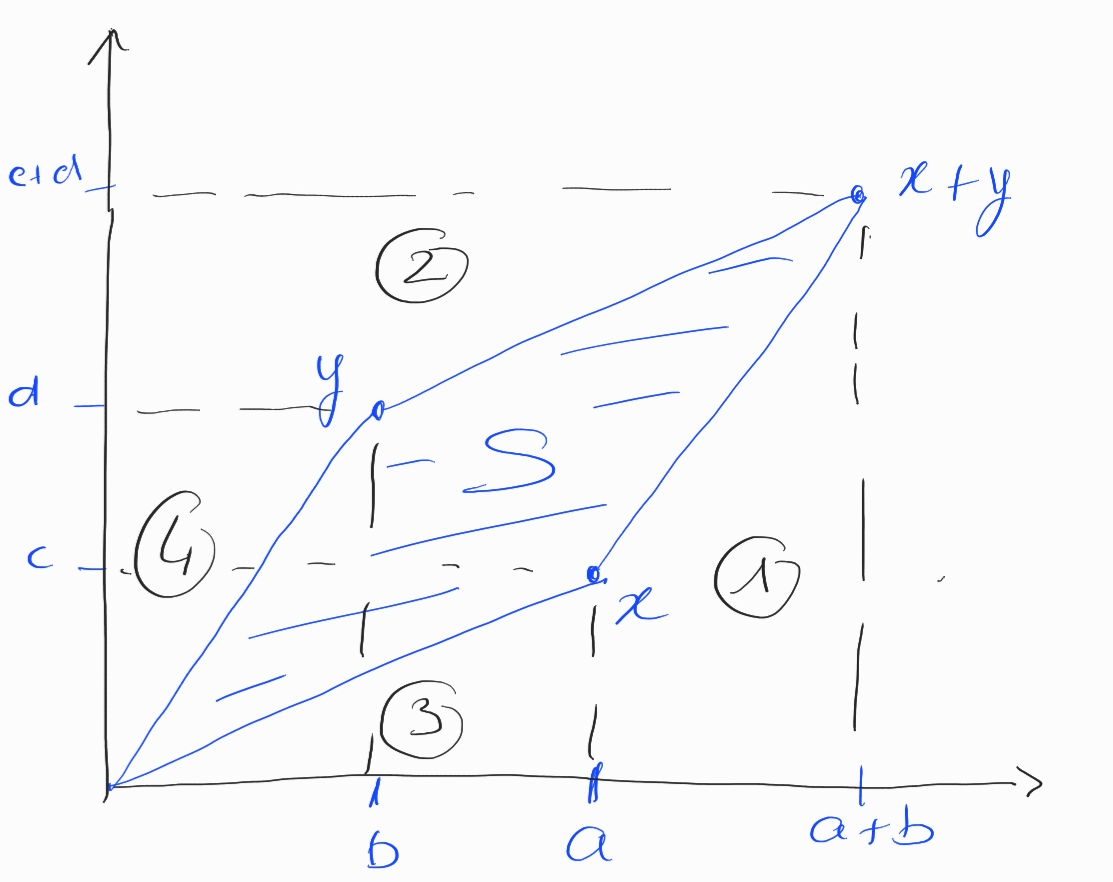
\includegraphics{DeterminantVolumeDimension2}
    $$
    soit
    \begin{align*}
      S 
      & = (a+b)(c+d) 
      - \underset{(1)}{\underbrace{b\left(c + \frac{d}2\right)}} 
      - \underset{(2)}{\underbrace{c\left(b + \frac{a}2\right)}} 
      - \underset{(3)}{\underbrace{\left(\frac{ac}2\right)}} 
      - \underset{(4)}{\underbrace{\left(\frac{bd}2\right)}} \\
      & = ac + bc + ad + bd - bc - \frac{bd}2 - bc - \frac{ac}2 - \frac{ac}2 - \frac{bd}2 \\
      & = ad - bc.
    \end{align*}
  \item En dimension $n$ : matrice diagonale = volume d'un parallélépipède.
  \end{itemize}
\end{enumerate}


\begin{proposition} \label{prop:formuleGeneraleDeterminant}
  \begin{equation} \label{eq:determinant}
    |A| = \sum_{\sigma \in \Scal_n} s(\sigma) \prod_{i=1}^n a_{i, \sigma(i)} 
    \end{equation}
    où $\Scal$ est l'ensemble des permutation de $\{1, \dots n\}$ et $s(\sigma) \in \{-1, +1\}$ désigne la signature de la permutation $\sigma$. 
\end{proposition}

La proposition \ref{prop:formuleGeneraleDeterminant} n'est pas démontrée ici. \eproof.

\remark
Le formule \eqref{eq:determinant} est rarement utilisée en pratique (notamment parce que $|\Scal| = n!$), sauf pour $n=2$ ou $n=3$.

%-------------------------------------------------------------------------------
%-------------------------------------------------------------------------------
\subsection{Calcul de déterminant de matrices $n \times n$} 
%-------------------------------------------------------------------------------

On s'intéresse ici au calcul effectif d'un déterminant.

\begin{proposition}[Déterminant par blocs] \label{prop:determinantParBlocs}
  Soit $A \in \Mcal_{n,n}$ de la forme
  $$
  A = \left[\begin{array}{cc}
      B & C \\ 0_{n-p, p} & D
    \end{array}\right]
  $$
  où $1 \leq p < n$, $B \in \Mcal_{p, p}$, $C \in \Mcal_{p, n-p}$, $0_{n-p, p}$ est l'élément nul de $\Mcal_{n-p, p}$, $D \in \Mcal_{n-p, n-p}$, on a
  $$
  |A| = |B| |D|.
  $$
\end{proposition}

\proof
La proposition \ref{prop:determinantParBlocs} est donnée sans démonstration. 
\eproof

\remark 
Intuitivement, elle repose sur la formule générale du déterminant \eqref{eq:determinant} : toute permutation $\sigma$ intervertissant un des $p$ premiers éléments avec un des $n-p$ derniers fait nécessaire intervenir un élément du bloc $0_{n-p, p}$ et le produit qui lui est associé est donc nul.

\remark Le déterminant de $A$ ne dépend donc pas des éléments de $C$.

\begin{proposition}[Déterminant d'une matrice triangulaire] \label{prop:determinantMatriceTriangulaire}
  Si $A \in \Mcal_{n,n}$ est triangulaire, 
  $$
  A = \prod_{i=1}^n a_{ii}.
  $$
\end{proposition}

% {Démonstration de la proposition \ref{prop:determinantMatriceTriangulaire}.}
\proof
En appliquant le calcul de déterminant par blocs par récurrence:
\begin{align*}
  |A| 
  & = 
  \left|\left[\begin{array}{c;{2pt/2pt}ccc}
                a_{11} & a_{12} & \dots & a_{1n} \\
                \hdashline[2pt/2pt]
                0 & a_{22} &  & a_{2n} \\
                \vdots  & \ddots & \ddots & \vdots \\
                0 & \dots & 0 & a_{nn} \\
              \end{array}\right]\right| 
  = a_{11} \times 
  \left|\left[\begin{array}{c;{2pt/2pt}ccc}
                a_{22} & a_{23} & \dots & a_{2n} \\
                \hdashline[2pt/2pt]
                0 & a_{33} &  & a_{3n} \\
                \vdots & \ddots & \ddots & \vdots \\
                0 & \dots & 0 & a_{nn} \\
              \end{array}\right]\right| \\
  & = a_{11} \times a_{22} \times 
  \left|\left[\begin{array}{c;{2pt/2pt}ccc}
                a_{33} & a_{34} & \dots & a_{3n} \\
                \hdashline[2pt/2pt]
                0 & a_{44} &  & a_{4n} \\
                \vdots  & \ddots & \ddots & \vdots \\
                0 & \dots & 0 & a_{nn} \\
              \end{array}\right]\right| 
  = \dots = a_{11} \times a_{22} \times \dots \times a_{n-1, n-1} \times a_{nn}.
\end{align*}
\eproof

\begin{definition}[Mineur et cofacteur] \label{def:mineurCofacteur}
  Pour une matrice $A \in \Mcal_n$, 
  \begin{enumerate}[\itemdot]
   \item on note $A^{(ij)}$ la matrice $A$ privée de sa $i$-ème ligne et de sa $j$-ème colonne,
   \item on appelle {\em mineur} le déterminant $|A^{(ij)}|$ et
   \item on appelle {\em cofacteur} de l'élément $(i, j)$, le produit $(-1)^{i+j} |A^{(ij)}|$.
  \end{enumerate}
\end{definition}

\begin{proposition}[Méthode des cofacteurs] \label{prop:methodeCofacteurs}
  Pour $A \in \Mcal_n$ et pour tout $i_0, j_0 \in \{1, \dots, n\}$, on a 
  \begin{align*}
    |A| 
    & = \sum_{j=1}^n a_{i_0j} (-1)^{i_0+j} |A^{(i_0j)}| & (\text{développement par rapport à la ligne $i_0$}) \\
    & = \sum_{i=1}^n a_{ij_0} (-1)^{i+j_0} |A^{(ij_0)}| & (\text{développement par rapport à la colonne $j_0$})
  \end{align*}
\end{proposition}

La démonstration de la proposition \ref{prop:methodeCofacteurs} sera faite en TD. \eproof

\remark Cette formule fournit une autre démonstration de l'équation \eqref{eq:determiantMatriceDiagonale} en développant successivement par rapport à chaque ligne : $D_n = \lambda_n D_{n-1}$.

\paragraph*{Exemples.}
\begin{itemize}
  \item Le déterminant de la matrice 
  \begin{align*}
    A_1 & = \left[\begin{array}{rrr}
      2 & -1 & 3 \\ 2 & -1 & 6 \\ -2 & 1 & 0
      \end{array}\right], &
  \end{align*}
  est nul car la première colonne est égale à $(-2)$ fois la seconde.
  \item Le déterminant de la matrice
  \begin{align*}
    A_2 & = \left[\begin{array}{rrr}
      2 & -1 & 3 \\ 2 & -1 & 6 \\ 1 & 0  & 2
      \end{array}\right]
  \end{align*}
  vaut $-3$, en développant par rapport à la dernière ligne :
  $$
  |A_2|
  = \left|\begin{array}{rrr}
    2 & -1 & 3 \\ 2 & -1 & 6 \\ 1 & 0  & 2
    \end{array}\right|
  = 1 \left|\begin{array}{rr} -1 & 3 \\ -1 & 6 \end{array}\right|
  + 2 \left|\begin{array}{rr} 2 & -1 \\ 2 & -1 \end{array}\right|
  = 1 \times (-3) + 2 \times 0 = -3.
  $$
\end{itemize}


%-------------------------------------------------------------------------------
%-------------------------------------------------------------------------------
\subsection{Inverse d'une matrice $n \times n$}
%-------------------------------------------------------------------------------

\begin{proposition} \label{prop:inverseMatriceCofacteurs}
  Soit $A \in \Mcal_n$ une matrice inversible, soit $B$ la matrice de ses cofacteurs : 
  $$
  B = [b_{ij}]_{1 \leq i, j \leq n}, \qquad 
  b_{ij} = (-1)^{i+j} |A^{(ij)}|.
  $$
  L'inverse de $A$ est égale à la transposée de la matrice de ses cofacteurs divisée par son déterminant : 
  $$
  A^{-1} = \frac1{|A|} B^\top.
  $$
\end{proposition}

% {Démonstration de la proposition \ref{prop:inverseMatriceCofacteurs}.} 
%   voir \url{https://www.techno-science.net/definition/5091.html}
\proof
La démonstration repose sur le calcul d'un élément quelconque du produit $C = A B^\top$. En notant $C = [c_{ik}]_{1 \leq i, k \leq n}$ : 
$$
c_{ik} 
= \sum_{j=1}^n a_{ij} b_{kj} 
= \sum_{j=1}^n (-1)^{j+k} a_{ij} |A^{(kj)}|.
$$
\begin{description}
  \item[$i = k$:] on reconnaît le calcul du déterminant de $A$ obtenu en développant par rapport à sa $i$-ème ligne : 
  $$
  c_{ik} 
  = \sum_{j=1}^n (-1)^{j+i} a_{ij} |A^{(ij)}|
  = |A|.
  $$
  \item[$i \neq k$:] 
%   on reconnaît $(-1)^{j+k} a_{ij} |A^{(kj)}|$ comme le déterminant, calculé par blocs, de la matrice
%   $$
%   \left[\begin{array}{ccccccc}
%          a_{1, 1} & \cdots & a_{1,j-1} & 0 & a_{1, j+1} & \cdots & a_{1, n} \\
%          \vdots & & \vdots & \vdots & \vdots &  & \vdots \\
%          a_{k-1,1} & \cdots & a_{k-1,j-1} & 0 & a_{k-1, j+1} & \cdots & a_{k-1, n} \\
%          0 & \cdots & 0 & a_{i, j} & 0 & \cdots & 0 \\
%          a_{k+1,1} & \cdots & a_{k+1,j-1} & 0 & a_{k+1, j+1} & \cdots & a_{k+1, n} \\
%          \vdots & & \vdots & \vdots & \vdots &  & \vdots \\
%          a_{n, 1} & \cdots & a_{n,j-1} & 0 & a_{n, j+1} & \cdots & a_{n, n} 
%         \end{array}\right]
%   $$
%   qui est égale à celui de la matrice
%   $$
%   D_i^{jk} = 
%   \left[\begin{array}{ccccccc}
%          a_{1, 1} & \cdots & a_{1,j-1} & a_{1, j} & a_{1, j+1} & \cdots & a_{1, n} \\
%          \vdots & & \vdots & \vdots & \vdots &  & \vdots \\
%          a_{k-1,1} & \cdots & a_{k-1,j-1} & a_{k-1, j} & a_{k-1, j+1} & \cdots & a_{k-1, n} \\
%          0 & \cdots & 0 & a_{i, j} & 0 & \cdots & 0 \\
%          a_{k+1,1} & \cdots & a_{k+1,j-1} & a_{k+1, j} & a_{k+1, j+1} & \cdots & a_{k+1, n} \\
%          \vdots & & \vdots & \vdots & \vdots &  & \vdots \\
%          a_{n, 1} & \cdots & a_{n,j-1} & a_{n, j} & a_{n, j+1} & \cdots & a_{n, n} 
%         \end{array}\right].
%   $$
%   On a notamment
%   \begin{align*}
%     D_1^{jk} 
%       & = \left[\begin{array}{cccc}
%             a_{1, 1} & a_{1,2} & \cdots & a_{1, n} \\
%             \vdots & \vdots & & \vdots \\
%             a_{k-1, 2}  & a_{k-1,2} & \cdots & a_{k-1, n} \\
%             a_{i, 1} & 0 & \cdots & 0 \\
%             a_{k+1, 1}  & a_{k+1,2} & \cdots & a_{k+1, n} \\
%             \vdots & \vdots & & \vdots \\
%             a_{n, 1}  & a_{n,2} & \cdots & a_{n, n} 
%             \end{array}\right], \quad
%     D_2^{jk} 
%       & = \left[\begin{array}{ccccc}
%             a_{1,1} & a_{1,2}  & a_{1,3} & \cdots & a_{1, n} \\
%             \vdots & \vdots & \vdots & & \vdots \\
%             a_{k-1,1} & a_{k-1,2}  & a_{k-1,3} & \cdots & a_{k-1, n} \\
%             0 & a_{i, 2} & 0 & \cdots & 0 \\
%             a_{k+1,1} & a_{k+1,2}  & a_{k+1,3} & \cdots & a_{k+1, n} \\
%             \vdots & \vdots & \vdots & & \vdots \\
%             a_{n,1} & a_{n,2}  & a_{n,3} & \cdots & a_{n, n} 
%         \end{array}\right].
%   \end{align*}
  soit $\widetilde{A} = [\widetilde{a}_{ij}]$ la matrice égale à la matrice $A$ dont la $k$-ème ligne est remplacée par la $i$-ème ligne ($\widetilde{a}_{i'j} = a_{i'j}$ si $i' \neq k$ et $\widetilde{a}_{kj} = a_{ij}$). Cette matrice possède deux lignes égales (la $i$-ème et la $k$-ème), donc son déterminant est nul : $|\widetilde{A}| = 0$. \\
  Mais, par développement le long de la $k$-ème ligne, puisque $\widetilde{a}_{kj} = a_{ij}$ et $\widetilde{A}^{kj}= A^{ij}$ pour tout $j$, on a
  $$
  |\widetilde{A}|
  = \sum_{j=1}^n (-1)^{k+j} \widetilde{a}_{kj} |\widetilde{A}^{kj}|
  = \sum_{j=1}^n (-1)^{k+j} \textcolor{red}{a_{ij}} |\textcolor{red}{A^{ij}}|
  = c_{ik}, 
  $$
  donc $c_{ik} = 0$.
\end{description}
On a ainsi montré que
$$
c_{ik} = \left\{\begin{array}{ll} 
                  |A| & \text{si $i = k$} \\
                  0 & \text{sinon}
                \end{array} \right.
\qquad \Leftrightarrow \qquad
C = AB^\top = |A| I
\qquad \Leftrightarrow \qquad
A^{-1} = B^\top \left/|A|\right..
$$
\eproof

\begin{lemma}
  L'inverse de la matrice diagonale $D = \diag(\mu_1, \dots \mu_n$) dont tous les termes diagonaux sont non nuls est la matrice diagonale $D^{-1} = \diag(\mu_1^{-1}, \dots \mu_n^{-1})$.
\end{lemma}

\proof
On vérifie que $D D^{-1} = D^{-1} D = I_n$.
\eproof

\newpage %-------------------------------------------------------------------------------
%-------------------------------------------------------------------------------
\section{Valeurs et vecteurs propres, diagonalisation} \label{sec:LinAlg-Eigen}
%-------------------------------------------------------------------------------
%-------------------------------------------------------------------------------

%-------------------------------------------------------------------------------
%-------------------------------------------------------------------------------
\subsection{Valeurs et vecteurs propres} \label{sec:ValVecPropres}
%-------------------------------------------------------------------------------

\begin{definition}[Valeur et vecteur propre]
  $\lambda \in \Rbb$ est une valeur propre de $A \in \Mcal_n(\Rbb)$ ssi, il existe un vecteur non nul $x \in \Rbb^n$ tel que $A x = \lambda x$. $x$ est appelé vecteur propre de $A$ associé à $\lambda$.
\end{definition}

\begin{exercise*}
  Donner $n$ valeurs propres (et les vecteurs propres associés) de la matrice 
  $$
  D = \diag(\mu_1, \mu_2, \dots, \mu_n).
  $$
\end{exercise*}

\solution{$\mu_1, \mu_2, \dots, \mu_n$ et les $n$ vecteurs respectifs de la base canonique.}

\begin{proposition}[Vecteur propre]
  Si $x$ est un vecteur de propre de $A$ associé à la valeur propre $\lambda$, $y = k x$ l'est également.
\end{proposition}

\proof 
  C'est une conséquence de la linéarité de la multiplication de $x$ par $A$ : 
  $$
  A y = A \times (k x) = k (A \times x) = k (\lambda x) = \lambda (k x) = \lambda y.
  $$
%   $x$ est un vecteur de propre de $A$ associé à la valeur propre $\lambda$ ssi, pour tout $1 \leq i \leq n$, 
%   $$
%   \sum_{j=1}^n a_{ij} x_j = \lambda x_i.
%   $$
%   Si $y = a x$, alors pour tout $1 \leq i \leq n$, $y_i = b x_i$, et donc
%   $$
%   \sum_{j=1}^n a_{ij} y_j 
%   = \sum_{j=1}^n a_{ij} b x_j
%   = b \sum_{j=1}^n a_{ij} x_j
%   = b \lambda x_i
%   = \lambda y_i.
%   $$
\eproof

\remarks
\begin{enumerate}
  \item Parler ``du'' vecteur propre $x$ associé à la valeur propre $\lambda$ est donc un abus de langage. Tous les vecteurs engendrés par $x$ sont également propres : on peut aussi parler plus précisément de {\em direction propre}. 
  \item Notamment, on peut toujours choisir des vecteurs propres de norme 1 $(\|v_i\| = 1$). 
  \item On peut aussi noter que, si $\lambda$ est valeur propre de $A$, l'équation
  \begin{equation} \label{eq:RqValeurPropre}
    Ax = \lambda x \qquad \Leftrightarrow \qquad (A - \lambda I)x = 0
  \end{equation}
  admet une infinité de solutions (tous les $kx$), donc que la matrice $A - \lambda I$ n'est pas inversible.
  \item La réciproque est d'ailleurs vraie: si $A - \lambda I$ n'est pas inversible, alors il existe un $y$ tel que $(A  - \lambda I)x_1 = y = (A - \lambda I)x_2$ avec $x_1 \neq x_2$. Par différence on a donc $(A  - \lambda I)(x_1 - x_2) = 0$, soit $A(x_1 - x_2) = \lambda(x_1 - x_2)$ et $\lambda$ est donc valeur propre de $A$ associée à $x_1 - x_2$.
\end{enumerate}

%-------------------------------------------------------------------------------
%-------------------------------------------------------------------------------
\subsection{Polynôme caractéristique} \label{sec:polCarac}
%-------------------------------------------------------------------------------

\begin{definition}[Polynôme caractéristique]
  Le polynôme caractéristique de la matrice $A \in \Mcal_n$ est l'application 
  $$
  \begin{array}{r|rcl}
   P_A: & \Rbb & \mapsto & \Rbb \\
    & \lambda & \to & |A - \lambda I_n|.
  \end{array}
  $$
\end{definition}

\bigskip
\begin{theorem}
  $\lambda$ est une valeur propre de la matrice $A$ ssi $P_A(\lambda) = 0$.
\end{theorem}

\proof 
  \begin{description}
    \item[$\Rightarrow$:] d'après la remarque de l'équation \eqref{eq:RqValeurPropre}, puisque $A - \lambda I$ n'est pas inversible, son déterminant $|A - \lambda I| = P_A(\lambda)$ est nul.
    \item[$\Leftarrow$:] $p_A(\lambda) = 0$ implique que $A - \lambda I$ n'est pas inversible, donc
      \begin{align*}
        & \exists y: (A - \lambda I)x = y \text{ admet plusieurs solutions $x$} \\
        & \Rightarrow \quad \exists x_1 \neq x_2: (A - \lambda I)x_1 = (A - \lambda I)x_2 = y \\
        & \Rightarrow \quad \exists z = (x_1 - x_2) \neq 0: (A - \lambda I)z = 0 
      \end{align*} 
      donc $\lambda$ est valeur propre de $A$. 
  \end{description}
%   \warning{Pb : théorème du rang non vu ici.} \\
%   On remarque tout d'abord que, par le théorème du rang ($\dim \text{Im}(A) + \dim \text{Ker}(A) = n)$, 
%   on a 
%   $$
%   \left\{\exists y: B x = y \text{ n'admet aucune solution}\right\} \Leftrightarrow \left\{\exists y': B x = y' \text{ admet plusieurs solutions}\right\}.
%   $$
%   Donc, pour toute matrice $B \in \Mcal_n$:
%   $$
%   \{B \text{ non inversible}\} \Leftrightarrow \{\exists y: B x = y \text{ admet plusieurs solutions}\}
%   $$
%   On a donc
%   \begin{align*}
%     p_A(\lambda) = 0 
%     & \quad \Leftrightarrow \quad |A - \lambda I| = 0 \\
%     & \quad \Leftrightarrow \quad A - \lambda I \text{ pas inversible} \\
%     & \quad \Leftrightarrow \quad \exists y: (A - \lambda I)x = y \text{ admet plusieurs solutions $x$} \\
%     & \quad \Leftrightarrow \quad \exists y: (A - \lambda I)(x_1 - x_2) = y-y = 0 \text{ admet une solution $(x_1, x_2): x_1 \neq x_2$} \\
%     & \quad \Leftrightarrow \quad \exists z \neq 0: (A - \lambda I)z = 0 \\
%     & \quad \Leftrightarrow \quad \exists z \neq 0: A z = \lambda z \\
%     & \quad \Leftrightarrow \quad \lambda \text{ valeur propre de } A. 
%   \end{align*} 
\eproof

\begin{exercise*}
  Soit la matrice diagonale $A$ de diagonale $(\mu_1, \dots, \mu_n)$.
  \begin{enumerate}
    \item Déterminer le polynôme caractéristique de $A$.
    \solution{
      $$
      P_A(\lambda) = \prod_{i=1}^n (\mu_i - \lambda).
      $$
    }
    \item En déduire ses valeurs propres.
    \solution{
      $$
      P_A(\lambda) = 0 \qquad \Leftrightarrow \qquad \lambda \in \{\mu_1, \dots \mu_n\}.
      $$
      }
    \item En déduire ses vecteurs propres.
      \solution{
        Ce sont les vecteurs de la base canoniques : 
        \begin{align*}
          e_1 & = \left[1 \; 0 \; \dots \; 0 \right], &
          e_i & = \left[0 \; \dots \; 0 \; 1 \; 0 \; \dots \; 0\right], & 
          e_n & = \left[0 \; \dots \; 0 \; 1 \right].
        \end{align*}
      }
  \end{enumerate}
\end{exercise*}

\progres{
Rappel cours 1
\begin{enumerate}
  \item Déterminant
  \begin{itemize}
    \item Inversibilité, déterminant
    \item Propriété du déterminant, calcul effectif
    \item Calcul de l'inverse d'une matrice
  \end{itemize}
  \item Valeurs et vecteur propres
  \begin{itemize}
    \item Polynôme caractéristique
  \end{itemize}    
\end{enumerate}
Programme cours 2
\begin{enumerate}
  \item Valeurs et vecteur propres
  \begin{itemize}
    \item Propriété du polynôme caractéristique
    \item Sous-espace propres
    \item Matrice diagonalisable
  \end{itemize}
  \item Matrices positives
  \begin{itemize}
    \item Au sens du produit scalaire
    \item Au sens de Perron-Frobenius
  \end{itemize}
\end{enumerate}
}

\begin{exercise*}
  Soit la matrice 
  $$
  A = \left[\begin{array}{rr} 1 & 1 \\ 3 & -1 \end{array}\right].
  $$
  \begin{enumerate}
   \item Déterminer le polynôme caractéristique de $A$.
   \solution{
   $$
   |A - \lambda I| 
   = \left|\begin{array}{cc} 1 - \lambda & 1 \\ 3 & -1 - \lambda \end{array}\right|
   = (1 - \lambda)(- 1 - \lambda) -3
   = \lambda^2 - 4.
   $$
   }
   \item En déduire ses valeurs propres.
  \solution{
    $$
    \lambda ^2 - 4 \qquad \Leftrightarrow \qquad \lambda \in \{-2, 2\}.
    $$
    }
   \item En déduire ses vecteurs propres.
    \solution{
      \begin{align*}
        \lambda & = -2 &
        \Rightarrow \; &
        \left\{\begin{array}{rl}
          x_1 + x_2 & = -2 x_1 \\
          3 x_1 - x_2 & = -2 x_2 
        \end{array} \right\} &
        \Rightarrow \; &
          x_2 = -3 x_1
        & \text{soit, par exemple, } u_1 & = \left[\begin{array}{r} 1 \\ -3 \end{array}\right], \\
        \lambda & = 2 &
        \Rightarrow \; &
        \left\{\begin{array}{rl}
          x_1 + x_2 & = 2 x_1 \\
          3 x_1 - x_2 & = 2 x_2 
        \end{array} \right\} &
        \Rightarrow \; &
          x_2 = x_1
        & \text{soit, par exemple, } u_2 & = \left[\begin{array}{r} 1 \\ 1 \end{array}\right]. 
      \end{align*}
    }
  \end{enumerate}
\end{exercise*}

\remark Les vecteurs et valeurs propres décrivent comment l'opérateur associé à la matrice $A$ agit sur un vecteur $x$ quelconque. \\
Dans l'exemple de l'exercice, les vecteurs propres 
$$
u_1 = \left[\begin{array}{r} 1 \\ -3 \end{array}\right]
\qquad \text{et} \qquad 
u_2 = \left[\begin{array}{r} 1 \\ 1 \end{array}\right]
$$
sont linéairement indépendants, donc on peut décomposer tout vecteur $x \in \Rbb^2$ en
$$
x = c u_1 + d u_2.
$$
Par linéarité, on a 
$$
A x = c A u_1 + d A u_2 = c \lambda_1 u_1 + d \lambda_2 u_2 = -3 c u_1 + 2 d u_2.
$$
La composante de $x$ dans la direction de $u_1$ est multipliée par $\lambda_1 = -2$ et sa composante dans la direction de $u_2$ est multipliée par $\lambda_2 = 2$.

\dessin{Transformation des deux composantes du vecteur $x = u_1 + 2u_2$ : 
$$
x = u_1 + 2u_2 = \left[\begin{array}{r} 3 \\ -1 \end{array}\right]
\qquad \Rightarrow \qquad
Ax = -2 u_1 + 4 u_2 =  \left[\begin{array}{r} 2 \\ 10 \end{array}\right].
$$
$$
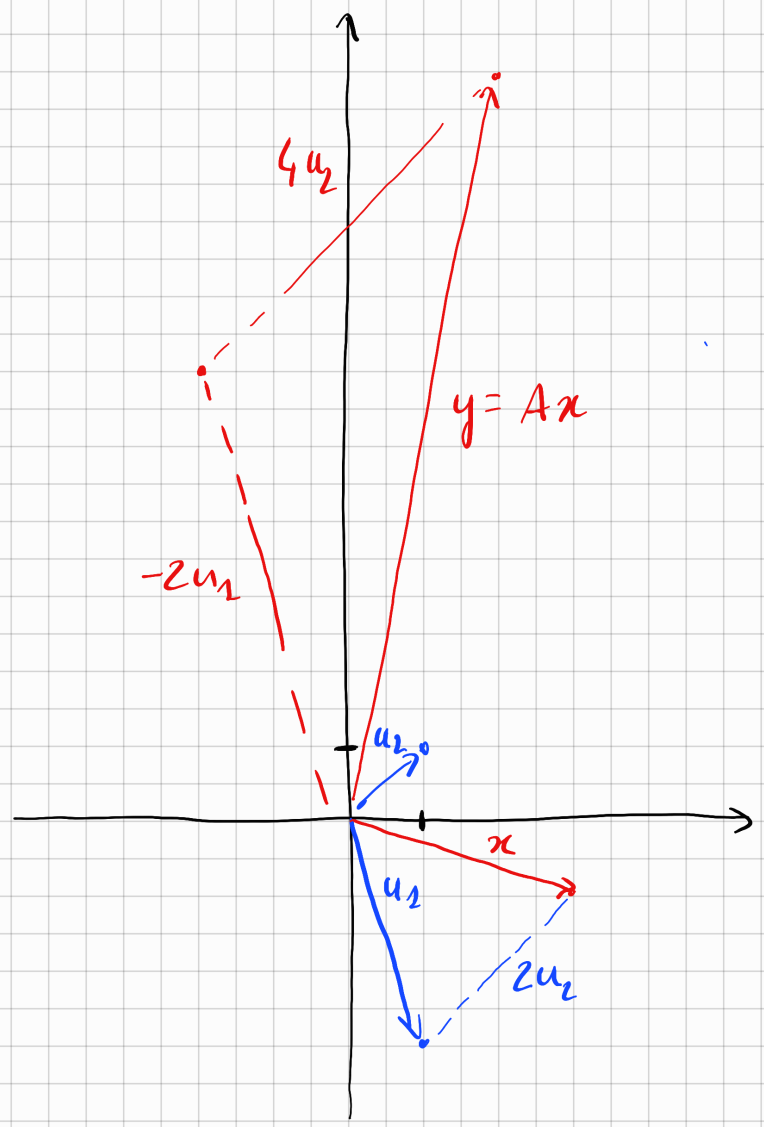
\includegraphics[width=0.5\textwidth]{TransformationComposantesVecteur}
$$
}

\newpage
\begin{definition}[Trace]
  La trace d'une matrice $A \in \Mcal_n$ est notée $\tr(A)$ et est égale à la somme de ses termes diagonaux :
  $$
  \tr(A) = \sum_{i=1}^n a_{ii}.
  $$
\end{definition}


\begin{exercise*}[Cas d'une matrice $2 \times 2$]
  On considère la matrice $A \in \Mcal_2$:
  $$
  A = \left[\begin{array}{cc} a & b \\ c & d\end{array}\right]
  $$
  Déterminer le polynôme caractéristique de $A$ et donner les conditions sur $p = \tr(A)$ et $q = \det(A)$ pour que $A$ admette deux valeurs propres réelles.
\end{exercise*}

\solution{
  On a 
  $$
  |A - \lambda I_2| 
  = \left|\begin{array}{cc} a - \lambda & b \\ c & d - \lambda \end{array}\right|
  = (a - \lambda)( d - \lambda) - bc
  = \lambda^2 - (a+d) \lambda + (ad - bc)
  = \lambda^2 - p \lambda + q
  $$
  qui admet deux solutions réelles (éventuellement égales) ssi
  $$
  p^2 - 4 q \geq 0
  \qquad \Leftrightarrow \qquad
  q \leq p^2 / 4.
  $$
  $$
%   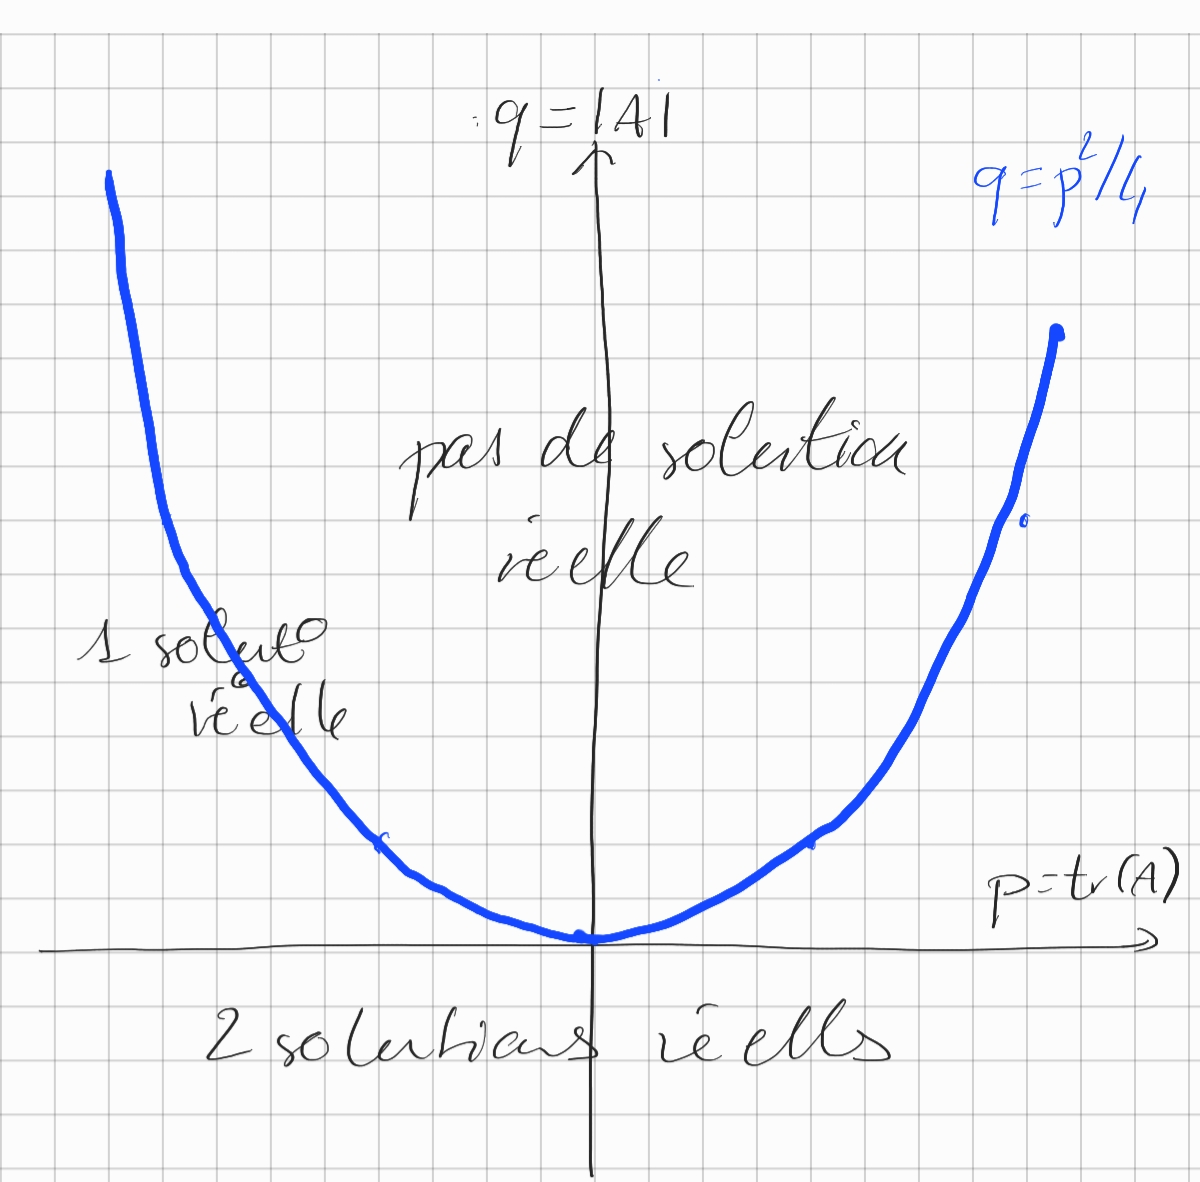
\includegraphics{ValeursPropresReellesDimension2} 
  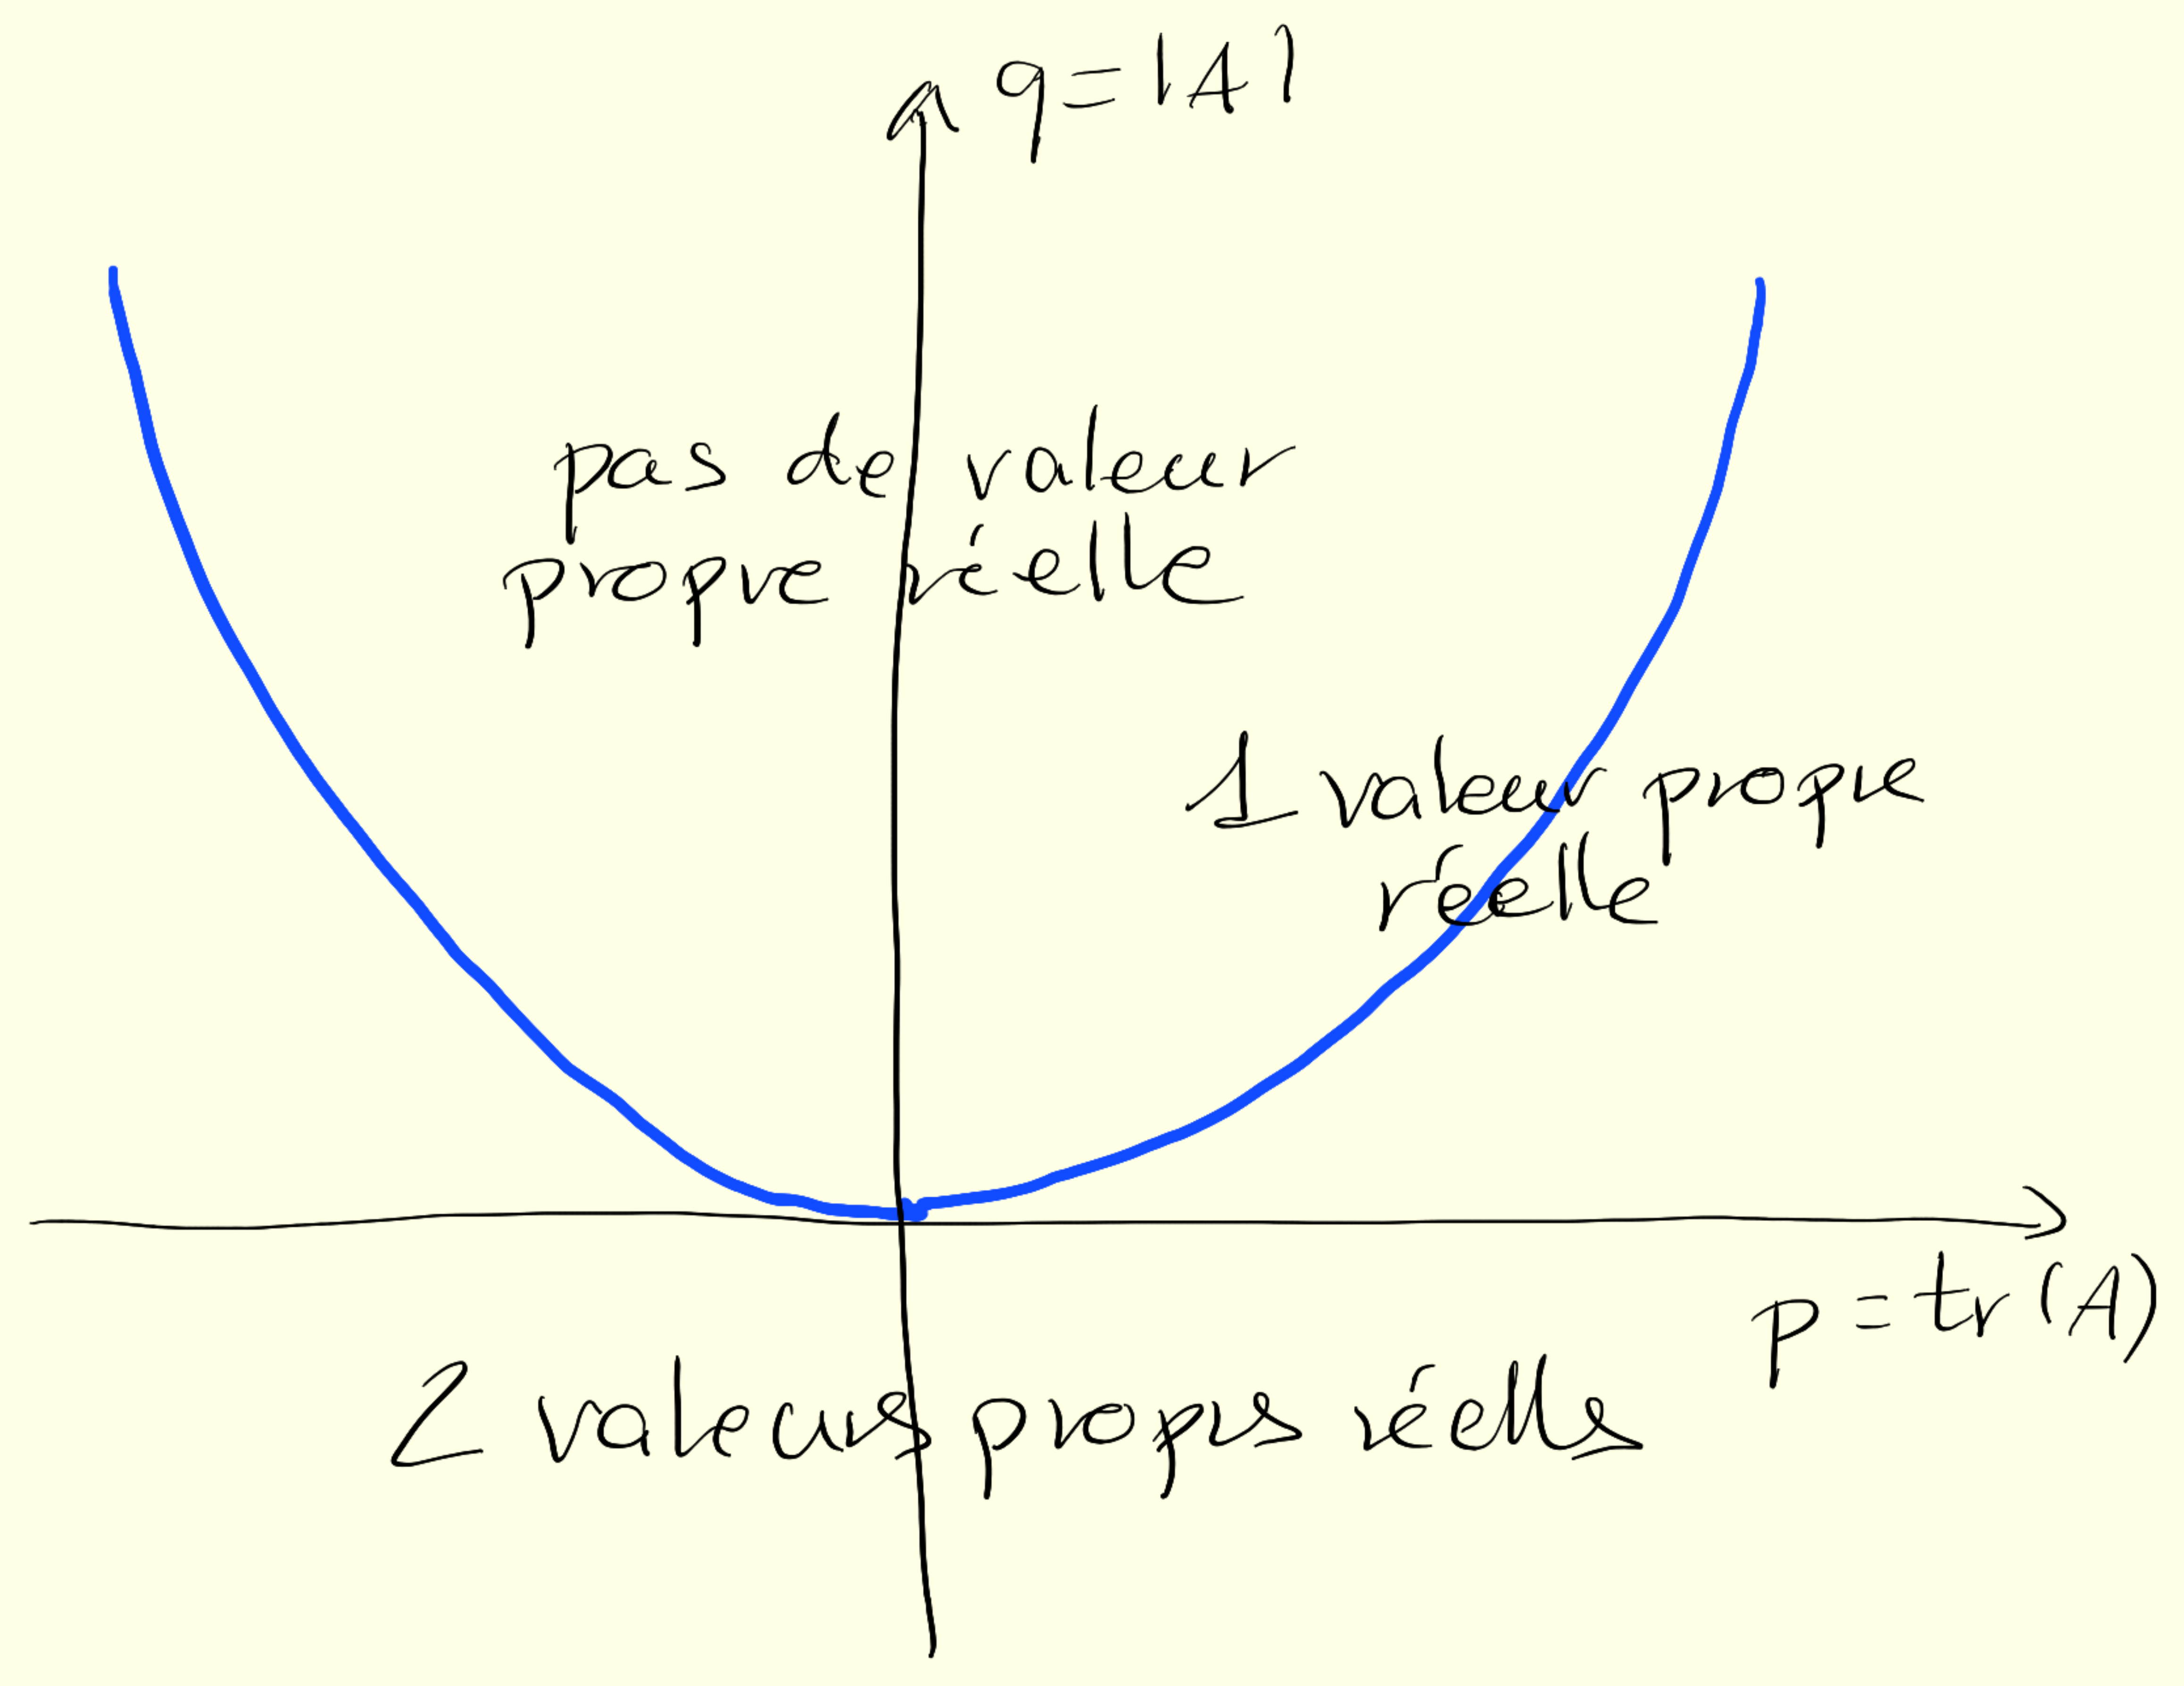
\includegraphics[width=0.5\textwidth]{ValeursPropresR2.png} 
  $$
}

\begin{exercise*}[Cas d'une matrice $2 \times 2$ symétrique]
  On considère la matrice $A \in \Mcal_2$:
  $$
  A = \left[\begin{array}{cc} a & b \\ b & c\end{array}\right]
  $$
  Montrer que ses deux valeurs propres sont réelles.
\end{exercise*}

\solution{D'après l'exercice précédent, il suffit de vérifier que
\begin{align*}
  p^2 - 4 q &
  = (a + c)^2 - 4(ac - b^2)
  = a^2 +2ac +c^2 - 4ac + 4b^2
  = (a - c)^2 + 4b^2 \geq 0,
\end{align*}
et $p^2 - 4 q = 0$ ssi $b = 0$ et $a=c$ (les deux valeurs propres étant alors égales à $a$).
}

\begin{theorem}[Propriétés du polynôme caractéristique]
  Le polynôme caractéristique $P_A$ de la matrice $A \in \Mcal_n(\Rbb)$ est de degré exactement $n$ et, en notant $[\lambda^k]P_A(\lambda)$ le coefficient d'ordre $k$ de $P_A(\lambda)$:
  $$
  [\lambda^n]P_A(\lambda) = (-1)^n, \qquad
  [\lambda^{n-1}]P_A(\lambda) = (-1)^{n-1} \tr(A), \qquad
  [\lambda^0]P_A(\lambda) = \det(A).
  $$
\end{theorem}

\proof
\begin{description}
  \item[Degré :] la formule \eqref{eq:determinant} montre que le degré de $P_A$ ne peut excéder $n$ puisque chaque permutation emprunte au plus $n$ termes diagonaux. La propriété suivante montre que le coefficient d'ordre $n$ est non nul.
  %
  \item[Coefficient de degré $n$ :] on raisonne par récurrence. Pour $n = 1$, on a bien $P_A(\lambda) = a_{11} - \lambda$. Si la propriété est vraie au rang $n-1$, on développe $|A - \lambda I_n|$ par rapport à la dernière ligne : 
  $$
  |A - \lambda I_n| 
  = \sum_{j=1}^{n-1} a_{nj} \underset{\scriptsize
    \begin{tabular}{c}\text{degré $\leq n-1$ par le même} \\
    \text{argument que précédemment}\end{tabular}
    }{\underbrace{|(A - \lambda I_n)^{(nj)}|}} + (a_{nn} - \lambda) \underset{\text{degré $= n-1$ par hypothèse}}{\underbrace{|(A - \lambda I_n)^{(nn)}|}}
  $$
  Donc
  $$
  [\lambda^n]|A - \lambda I_n| 
  = [\lambda^n](-\lambda |(A - \lambda I_n)^{(nn)}|) 
  = - [\lambda^{n-1}]\underset{\text{$= (-1)^{n-1}$ par hypothèse}}{\underbrace{(|(A - \lambda I_n)^{(nn)}|)}}
  = (-1)^n
  $$
  et le degré de $P_A$ est donc supérieur ou égal à $n$.
  %
  \item[Coefficient de degré $n-1$ :] cette propriété sera démontrée en TD.
  %
  \item[Coefficient de degré $0$ :] on remarquant que
    $$
    [\lambda^0]P_A(\lambda) = P_A(0) = |A - 0 I_n| = |A|.
    $$
\end{description}
% \begin{enumerate}[\itemdot]
%  \item La propriété $[\lambda^0]P_A(\lambda) = \det(A)$ est immédiate en se remarquant que
% $$
% [\lambda^0]P_A(\lambda) = P_A(0) = |A - 0 I_n| = |A|.
% $$
% \item La formule \eqref{eq:determinant} montre que le degré de $P_A$ ne peut excéder $n$ puisque chaque permutation emprunte au plus $n$ termes diagonaux.
% \item \SR{}{Exhiber l'unique chemin qui donne un terme en $\lambda^n$.}\\
% \SR{Les autres propriétés se montrent par récurrence en commençant par remarquer qu'elles sont toutes vraies pour $n = 2$ (cf Exercice 1.3.3). Pour la récurrence, on développe $|A - \lambda I_n|$ par rapport à la dernière ligne : 
% $$
% |A - \lambda I_n| 
% = \sum_{j=1}^{n-1} a_{nj} \underset{\scriptsize
%   \begin{tabular}{c}\text{degrée $\leq n-1$ par \eqref{eq:determinant}} \\
%   \text{car aucune permutation n'emprunte} \\
%   \text{2 fois la même ligne ou la même colonne}\end{tabular}
%   }{\underbrace{|(A - \lambda I_n)^{(nj)}|}} + (a_{nn} - \lambda) \underset{\text{degrée $= n-1$ par hypothèse}}{\underbrace{|(A - \lambda I_n)^{(nn)}|}}
% $$
% Donc
% $$
% [\lambda^n]|A - \lambda I_n| 
% = [\lambda^n](-\lambda |(A - \lambda I_n)^{(nn)}|) 
% = - [\lambda^{n-1}]\underset{\text{$= (-1)^{n-1}$ par hypothèse}}{\underbrace{(|(A - \lambda I_n)^{(nn)}|)}}
% = (-1)^n
% $$
% et le degré de $P_A$ est donc supérieur ou égal à $n$.}{}
% \item \SR{La démonstration pour le coefficient d'ordre $n-1$ ($= [\lambda^{n-1}]P_A(\lambda)$) suit le même principe.}{[Voir TD]}
% \end{enumerate}
\eproof

%-------------------------------------------------------------------------------
\subsubsection{Rappel sur les polynômes} 
%-------------------------------------------------------------------------------

\begin{proposition}[Polynômes à coefficients réels]
  Tout polynôme à coefficients réels est scindé sur $\Cbb$, c'est à dire que, pour $P$ de degré exactement $n$, il existe un réel $a$ non nul et $n$ nombres complexes $x_1, \dots, x_n$ (non nécessairement distincts) tels que
  $$
  P(x) = a \prod_{i=1}^n (x_i - x).
  $$
  $x_1, \dots, x_n$ sont des racines de $P$.
\end{proposition}

\proof
Non démontré
\eproof

\begin{corollary*}[Polynôme caractéristique]
  Le polynôme caractéristique $P_A$ d'une matrice réelle s'écrit
  $$
  P_A(\lambda) = \prod_{i=1}^n (\lambda_i - \lambda)
  $$
  où les $\lambda_i$ sont les $n$ valeurs propres (non nécessairement distinctes, ni réelles) de $A$.
\end{corollary*}

\proof
Les $\lambda_i$ sont les racines de $P_A$ et le coefficient $a$ vaut 1 puisque $[\lambda^n]P_A(\lambda) = (-1)^n$.
\eproof

\begin{definition}[Ordre de multiplicité]
  On note $d$ le nombre de racines distinctes d'un polynôme $P$ de degré $n$ et $x_1, x_2, \dots x_d$ ces racines. On peut alors écrire $P$ sous la forme
  $$
  P(x) = a \prod_{j=1}^d (x_j - x)^{m_j}
  $$
  et $m_j$ est appelé ordre de multiplicité de la racine $x_j$ et les $m_j$ vérifient $ \sum_{j=1}^d m_j = n$.
\end{definition}

%-------------------------------------------------------------------------------
\paragraph*{Exemple.} 
$$
P(x) = x^3 - 4x^2 + 5x - 2 = - (2-x)(1-x)^2
$$ 
admet $x_1 = 1$ et $x_2 = 2$ pour racines avec $m_1 = 2$ et $m_2 = 1$.


\begin{corollary*}[Polynôme caractéristique]
  Le polynôme caractéristique $P_A$ d'une matrice réelle s'écrit
  $$
  P_A(\lambda) = \prod_{j=1}^d (\lambda_j - \lambda)^{m_j}
  $$
  où les $\lambda_j$ sont les $d$ valeurs propres distinctes de $A$.
\end{corollary*}

\proof
Directe.\eproof

\begin{corollary*}
  Le déterminant est égal au produit des valeurs propres : 
  $$
  |A| = \prod_{i=j}^d \lambda_j^{m_j}.
  $$
\end{corollary*}

\proof
  Du fait des propriétés du polynôme caractéristique et de sa factorisation, on a
  $$
  |A| = [\lambda^0]P_A(\lambda) = P_A(0) = \prod_{j=1}^d \lambda_j^{m_j}.
  $$
\eproof

%-------------------------------------------------------------------------------
\subsubsection{Sous-espaces propres} 
%-------------------------------------------------------------------------------

\begin{definition}[Sous-espace propre]
  On appelle sous-espace propre associé à la valeur propre $\lambda$, l'ensemble des vecteurs propres associés à $\lambda$ :
  $$
  \Ecal(\lambda) = \{x \in \Rbb: Ax = \lambda x\},
  $$
  qui est aussi le noyau de $A - \lambda I$ : 
  $$
  \Ecal(\lambda) = \{x \in \Rbb: (A - \lambda I)x = 0\} = \text{Ker}(A - \lambda I).
  $$
\end{definition}

\begin{proposition}[Intersection des espaces propres]
  Soit deux valeurs propres distinctes $\lambda_1$ et $\lambda_2$ d'une matrice $A \in \Mcal_n(\Rbb)$:
  $$
  \Ecal(\lambda_1) \cap \Ecal(\lambda_2) = 0_n.
  $$
\end{proposition}

\proof
Directe car $Ax = \lambda_1 x = \lambda_2 x$ avec $\lambda_1 \neq \lambda_2$ ssi $x = 0$.
\eproof


\begin{proposition}[Dimension de l'espace propre]
  Pour toute matrice $A \in \Mcal_n(\Rbb)$ et pour chacune de ses valeurs propres, 
  $$
  \dim(\Ecal(\lambda_i)) \leq m_i.
  $$
\end{proposition}

\proof
Non démontré
\eproof


\remarks
\begin{enumerate}
  \item L'action d'une matrice $A$ dans chacun de ces sous-espaces est une simple homothétie si la valeurs propres associée est réelle.
  \item On sait donc que les différentes valeurs propres sont associées à des sous-espaces propres qui engendrent un sous-espace de $\Rbb^n$, mais pas nécessairement $\Rbb^n$ tout entier. 
  \item On s'intéresse notamment aux matrices dont toutes les valeurs propres sont réelles et dont la réunion des espaces propres engendre $\Rbb^n$.
\end{enumerate}

%-------------------------------------------------------------------------------
%-------------------------------------------------------------------------------
\subsection{Matrices diagonalisables} \label{sec:MatDiag}
%-------------------------------------------------------------------------------

\begin{definition}[Matrice diagonalisable] \label{def:matriceDiagonalisable}
  Une matrice $A \in \Mcal_n(\Rbb)$ est dite diagonalisable s'il existe un matrice $\Lambda \in \Mcal_n(\Rbb)$ diagonale et une matrice $P \in \Mcal_n(\Rbb)$ inversible telles que
  $$
  A = P \Lambda P^{-1}.
  $$
\end{definition}

\begin{proposition}
  Les termes diagonaux de la matrice $\Lambda$ sont les valeurs propres de $A$ et les colonnes de la matrice $P$ sont les vecteurs propres associés :
  en notant $\Lambda = \diag(\lambda_1, \dots \lambda_n)$ et $P = [u_1 \dots u_n]$, 
  $$
  \forall \; 1 \leq j \leq n: \quad A u_j = \lambda_j u_j.
  $$
\end{proposition}

\proof
  On calcule tous les produits $A u_i$ simultanément : 
  $$
  A P 
  = P \Lambda P^{-1} P 
  = P \Lambda
  = [\lambda_1 u_1 \; \lambda_2 u_2 \; \dots \lambda_n u_n],
  $$
  en se rappelant que la multiplication à droite par une matrice diagonale multiple chaque colonne par le terme diagonal correspondant. On a donc bien $A u_i = \lambda_i u_i$ pour chaque $1 \leq i \leq n$. \\
\eproof

\remark
$A$ admet au plus $n$ valeurs propres et les $\lambda_i$ sont au nombre de $n$, donc les $\lambda_i$ sont bien {\em les} valeurs propres de $A$.

\remark
Une matrice $A$ est diagonalisable si son application consiste à
\begin{description}
 \item[$P^{-1}$:] Passer de la base canonique à la base constituée des vecteurs colonnes de $P$, qui sont les vecteurs propres,
 \item[$\Lambda$:] Appliquer à chaque coordonnée de la nouvelle base une homothétie de rapport $\lambda_i$,
 \item[$P$:] Revenir dans la base canonique.
\end{description}

% \begin{proposition}
%   Le déterminant d'une matrice diagonalisable est égal au produit de ses valeurs propres.
% \end{proposition}

% \proof
% D'après la définition, les valeurs propres de $A$ sont les éléments diagonaux de la matrice $\Lambda$. On observe alors que
% $$
% |A| = |P \Lambda P^{-1}| = |P| |P^{-1}| |\Lambda| = |\Lambda| = \prod_i \lambda_i.
% $$
% \eproof

\begin{proposition}
  Si la matrice $A$ est diagonalisable ($A = P \Lambda P^{-1}$), son inverse vaut $A^{-1} = P \Lambda^{-1} P^{-1}$.
\end{proposition}

\proof
On vérifie que $A A^{-1} = P \Lambda P^{-1} P \Lambda^{-1} P^{-1} = P \Lambda \Lambda^{-1} P^{-1} = P P^{-1} = I_n$.
\eproof

\begin{theorem}[Matrice diagonalisable]
  La matrice $A \in \Mcal_n(\Rbb)$ est diagonalisable ssi 
  \begin{enumerate}
   \item toutes ses valeurs propres $\lambda_i$ sont réelles et, 
   \item pour chacune d'elles, le sous-espace propre associé a pour dimension son ordre de multiplicité : 
   $$
   \dim(\Ecal(\lambda_i)) = m_i.
   $$
  \end{enumerate}
\end{theorem}

\proof
Non démontré
\eproof

\remark
Le résultat est intuitif en reprenant la définition \ref{def:matriceDiagonalisable} et en remarquant que chaque $\lambda_i$ distinct apparaît alors $m_i$ fois dans la diagonale de $\Lambda$ et qu'on peut donc lui associer $m_i$ vecteurs colonnes de $P$, qui engendrent bien un espace de dimension $m_i$, puique que $P$ est inversible.

\begin{corollary*}
  Toute matrice $A \in \Mcal_n(\Rbb)$ dont les $n$ valeurs propres sont réelles et distinctes ($m_i = 1$, pour tout $i = 1 \dots n$) est diagonalisable.
\end{corollary*}

\proof
Tous les sous-espaces propres sont de dimension au moins 1 (puisqu'il existe un vecteur non nul tel que $Ax = \lambda_i x$). Comme la dimension d'un sous-espace propre ne peut pas excéder l'ordre de multiplicité, les deux valeurs coïncident et valent 1.
\eproof

\begin{corollary*}
  Si la matrice $A \in \Mcal_n(\Rbb)$ est diagonalisable, l'ensemble des sous-espaces propres engendrent $\Rbb^n$ tout entier.
\end{corollary*}

\proof
C'est une conséquence de la proposition selon laquelle les intersections des sous-espaces propres sont réduites au vecteur nul.
\eproof

%-------------------------------------------------------------------------------
\paragraph*{Exemple de matrices non diagonalisables.}
\begin{enumerate}
 \item Soit
 $$
 A = \left[\begin{array}{cc} 1 & 1 \\ 0 & 1 \end{array}\right],
 \qquad 
 P_A(\lambda) 
 = \left|\begin{array}{cc} 1-\lambda & 1 \\ 0 & 1-\lambda \end{array}\right|
 = (1 - \lambda)^2
 $$
 donc $\lambda_1 = 1$ est valeur propre d'ordre de multiplicité 2, mais
 $$
 Ax = \lambda_1 x \quad \Leftrightarrow \quad 
 \left\{\begin{array}{rcl} x_1 + x_2 & = & x_1 \\ x_2 & = & x_2 \end{array} \right. \quad \Leftrightarrow \quad 
 x_2 = 0
 \qquad (\text{soit } u_1 = e_1)
 $$
 donc le sous-espace propre associé est de dimension 1.
 \item Soit 
 $$
 A = \left[\begin{array}{rrr} 0 & 1 & 0 \\ 0 & 0 & 1 \\ 0 & 0 & 0 \end{array}\right],
 \qquad 
 P_A(\lambda) 
 = \left|\begin{array}{rrr} -\lambda & 1 & 0 \\ 0 & -\lambda & 1 \\ 0 & 0 & -\lambda \end{array}\right|
 = -\lambda^3
 $$
 donc $\lambda_1 = 0$ est valeur propre d'ordre de multiplicité 3, mais
 $$
 A x = \lambda_1 x \quad \Leftrightarrow \quad 
 \left\{\begin{array}{rcl} x_2 & = & 0 \\ x_3 & = & 0 \end{array} \right.
 $$
 donc le sous-espace propre associé est de dimension 1.
 \item Soit la matrice {\em circulante}
 $$
 A = \left[\begin{array}{rrr} 0 & 1 & 0 \\ 0 & 0 & 1 \\ 1 & 0 & 0 \end{array}\right],
 \qquad 
 P_A(\lambda) 
 = \left|\begin{array}{rrr} -\lambda & 1 & 0 \\ 0 & -\lambda & 1 \\ 1 & 0 & -\lambda \end{array}\right|
 = -\lambda^3 + 1
 $$
 qui s'annule pour 
 $$
 \lambda \in \left\{1, \frac{-1+i\sqrt{3}}{2}, \frac{-1-i\sqrt{3}}{2}, \right\}.
 $$
 Le sous-espace propre associé à $\lambda_1$ est dit {\em invariant} et correspond à la première bissectrice : 
 $$
 A x = \lambda_1 x \quad \Leftrightarrow \quad 
 \left\{\begin{array}{rcl} x_2 & = & x_1 \\ x_3 & = & x_2 \\ x_1 & = & x_3 \end{array} \right.
 $$
 L'action de $A$ dans les autres dimensions est une rotation.
\end{enumerate}

% \begin{exercise*}
%   Déterminer les polynômes caractéristiques des matrices suivantes et en déduire si elles sont diagonalisables ou non.
%   \begin{align*}
%     A_1 & = \left[\begin{array}{ccc}
%       2 & -1 & 3 \\ 2 & -1 & 6 \\ 1 & 0  & 2
%       \end{array}\right], &
%     A_2 & = \left[\begin{array}{ccc}
%       1 & 1 & 0 \\ -5 & -2 & 5 \\ -1 & 0 & 2
%       \end{array}\right], \\ 
%     %
%     A_3 & = \left[\begin{array}{ccc}
%       -1 & 3 & 1 \\ 0 & 2 & 1 \\ 0 & 3 & 0
%       \end{array}\right], & 
%     A_4 & = \left[\begin{array}{ccc}
%       -1 & 3 & 1 \\ 0 & 2 & 1 \\ \alpha & \beta & 2
%       \end{array}\right],  
%   \end{align*}
% \end{exercise*}

\begin{exercise*}
  Déterminer le polynôme caractéristique de la matrice
  $$
  A = \left[\begin{array}{rrr}
  -1 & 3 & 1 \\ 0 & 2 & 1 \\ 0 & 3 & 0
  \end{array}\right], 
  $$
  et en déduire si elle est diagonalisable ou non.
\end{exercise*}

\solution{
  $$
  P_A(\lambda) 
  = \left|\begin{array}{rrr}
    -1-\lambda & 3 & 1 \\ 0 & 2-\lambda & 1 \\ 0 & 3 & -\lambda
      \end{array}\right|
  = (-1 - \lambda)(-\lambda (2 - \lambda) - 3)
  % = -(1 + \lambda)(\lambda^2 - 2\lambda - 3)
  = -(1 + \lambda)^2(\lambda - 3)
  $$
  donc les valeurs propres sont $\lambda_1 = -1$ et $\lambda_2 = 3$ avec $m_1 = 2$, $m_2 = 1$ et, pour $\lambda_1 = 1$, on a
  $$
  Ax = -x \quad\Leftrightarrow \quad 
  \left\{\begin{array}{rcl}
    -x_1 + 3x_2 + x_3 & = & -x_1 \\
    2x_2 + x_3 & = & -x_2 \\
    3x_2 & = & -x_3 \\
  \end{array}\right. \quad\Leftrightarrow \quad 
  3x_2 = -x_3
  $$
  donc $\dim(\Ecal(\lambda_1)) = 2 = m_1$ et $A$ est donc diagonalisable.

  Deux vecteurs propres (indépendants) associés à $\lambda_1$ sont
  $$
  [0 \; 1 \; -3]^\top \qquad \text{et} \qquad [1 \; 1 \; -3]^\top 
  $$
  et un vecteur propre associé à $\lambda_2$ est 
  $$
  [1 \; 1 \; 1]^\top.
  $$
  On peut diagonaliser $A = P \Lambda P^{-1}$ avec
  $$
  \Lambda = \left[\begin{array}{rrr}
  -1 & 0 & 0 \\ 0 & -1 & 0 \\ 0 & 0 & 3
  \end{array}\right]
  \qquad \text{et} \qquad 
  P = \left[\begin{array}{rrr}
  0 & 1 & 1 \\ 1 & 1 & 1 \\ -3 & -3 & 1
  \end{array}\right].
  $$
}

\begin{theorem}[Matrices réelles symétriques]
  Toute matrice $A \in \Mcal_n(\Rbb)$ symétrique ($A = A^\top$) est diagonalisable et ses vecteurs propres sont orthogonaux. 
\end{theorem}

\proof
Non démontrée (programme de classe prépa BCPST). 
% Voir Fre14-Notes-SymmetricMatricesAndEigendecomposition, section2, propositions 3 et 4.
\SRcorrect{\begin{itemize}
  \item Valeurs propres réelles : le polynôme caractéristique de $A$ admet au plus $n$ racines éventuellement multiples et complexes. Si $\lambda$ est une valeur propre de $A$, en notant $\overline{\lambda}$ le conjugué de $\lambda$ ($\overline{\lambda} = \lambda \Leftrightarrow \lambda \in \Rbb$), il existe un vecteur $x$ tel que
  \begin{align*}
    Ax & = \lambda x & 
    \Rightarrow \qquad \overline{Ax} & = \overline{\lambda x} &
    \Rightarrow \qquad A \overline{x} & = \overline{\lambda} \overline{x} \\
    \Rightarrow \qquad x^\top A \overline{x} & = \overline{\lambda} x^\top \overline{x}
  \end{align*}
  puisque $A$ est réelle et que $\overline{a b} = \overline{a} \overline{b}$. De même on a
  \begin{align*}
    Ax & = \lambda x & 
    \Rightarrow \qquad \overline{x}^\top A x & = \lambda \overline{x}^\top x &
    \Rightarrow \qquad x^\top A \overline{x} & = \lambda \overline{x}^\top x
  \end{align*}
  puisque $A$ est symétrique. On a donc $\overline{\lambda} x^\top \overline{x} =  \lambda \overline{x}^\top x$ avec $\overline{x}^\top x \neq 0$, donc $\overline{\lambda} = \lambda$, donc $\lambda$ est réelle.
  \item \todo{}
\end{itemize}}{}
\eproof

\remark
Puisque les vecteurs propres sont orthogonaux deux à deux, si on choisit des vecteurs propres $u_1, \dots u_n$ de norme 1, les colonnes de la matrice de passage $P$ constituent une base orthonormée de $\Rbb^n$. 

\newpage %-------------------------------------------------------------------------------
%-------------------------------------------------------------------------------
\section{Matrices positives} \label{sec:LinAlg-Pos}
%-------------------------------------------------------------------------------
%-------------------------------------------------------------------------------

\remark Il existe deux acceptions du terme ``matrice positive'' :
\begin{enumerate}[$\bullet$]
  \item matrice positive au sens du produit scalaire $A \succcurlyeq 0$
  \item matrice positive au sens de Perron-Frobénius $A \geq 0$
\end{enumerate}


%-------------------------------------------------------------------------------
%-------------------------------------------------------------------------------
\subsection{Matrices positives (au sens du produit scalaire : $A \succcurlyeq 0$)} 
%-------------------------------------------------------------------------------

\begin{definition}[Matrice positive] \label{def:matricePositive}
  Une matrice {\em symétrique} $A \in \Mcal_n$ est dite positive ($A \succcurlyeq 0$) ssi, 
  $$
  \forall x \in \Rbb: \quad x^\top A x \geq 0.
  $$
  Une matrice {\em symétrique} $A \in \Mcal_n$ est dite définie positive ($A \succ 0$) ssi, elle est positive et 
  $$
  x^\top A x = 0 \qquad \Leftrightarrow \qquad x = 0.
  $$
\end{definition}

\remark
On peut se demander pourquoi on restreint la définition aux matrices symétriques. La raison est que seule la {\em partie positive} d'une matrice intervient dans la définition de la positivité. \\
Pour s'en convaincre il suffit d'observer qu'on peut décomposer toute matrice $A$  en $A = S + T$ où $S$ est symétrique ($S = S^\top$) et $T$ est anti-symétrique ($T = -T^\top$) en prenant
$$
S = (A + A^\top) / 2, \qquad T = (A - A^\top) / 2
$$
(on peut d'ailleurs montrer que cette décomposition est unique). \\
La {\em forme quadratique} $x^\top A x$ s'écrit alors
\begin{align*}
  x^\top A x 
  & = x^\top S x + x^\top T x 
\end{align*}
où le second terme $x^\top T x$ est nul puisque, $x^\top T x$ étant un scalaire, il est égal à sont transposé, et donc
$$
x^\top T x = (x^\top T x)^\top = x^\top T^\top x = x^\top (- T) x = - x^\top T x.
$$


\begin{proposition}
  Si $A$ est (symétrique) positive, toutes ses valeurs propres sont positives ou nulles. \\
  Si elle est définie positive toutes ses valeurs propres sont strictement positives.
\end{proposition}

\proof
$\lambda$ est une valeur propre de $A$ ssi, il existe $x \neq 0$ tel que
$$
Ax = \lambda x \qquad \Rightarrow \qquad x^\top A x = \lambda x^\top x,
$$
or $x^\top A x \geq 0$ et $x^\top x > 0$ donc $\lambda \geq 0$. Si, de plus, $A$ est définie positive, $x^\top A x > 0$ pour tout $x$ non nul et donc $\lambda > 0$.
\eproof

% \begin{proposition}[Matrice positive symétrique]
%   Si $A$ est positive ($A \succcurlyeq 0$) et symétrique ($A = A^\top$), elle est est diagonalisable. De plus ses valeurs propres sont positives et ses vecteurs propres sont orthogonaux deux à deux.
% \end{proposition}
% 
% \proof
% Il suffit de combiner le dernier théorème de la section \ref{sec:MatDiag} avec la proposition précédente.
% \eproof

% \begin{proposition}[Inverse d'un matrice orthonormale] \todo{A faire en TD}
%   Si $P \in \Mcal_n$ est orthonormale, alors $P^{-1} = P^\top$.
% \end{proposition}

% \proof
% En notant $P = [v_{ij}]$, $v_j$ le $j$-ème vecteur colonne de $P$ et $B = [b_{ij}] = P^\top P$, on a
% $$
% P^\top = [v_{ji}] 
% \quad \Rightarrow \quad
% b_{ik} 
% = \sum_{k=1}^n [P^\top]_{ik} [P]_{kj} 
% = \sum_{k=1}^n v_{ki} v_{kj}
% = < v_i, v_j >
% = \left\{\begin{array}{rl} 1 & \text{si } i = j \\ 0 & \text{sinon} \end{array}\right.
% $$
% (puique les vecteurs $v_j$ sont orthonormés), donc $P^\top P = B = I$. La démonstration de $P P^\top = I$ est symétrique.
% \eproof

%-------------------------------------------------------------------------------
\subsubsection{Matrice de variance-covariance}
%-------------------------------------------------------------------------------

On revient à l'étude des matrices de variance-covariance introduite à la section \ref{sec:MatCov}.

\begin{proposition}[Matrice de variance-covariance]
  Soit $\Sigma$ la matrice de variance-covariance d'un vecteur aléatoire $X = [X_1, \dots X_n]^\top$.
  \begin{enumerate}
    \item $\Sigma$ est diagonalisable ;
    \item $\Sigma$ est positive : $\Sigma \succcurlyeq 0$ ;
    \item $\Sigma$ est définie positive sauf si une des $n$ variables est une fonction déterministe des $n-1$ autres.
  \end{enumerate}
\end{proposition}

\proof
\begin{enumerate}
\item Cela résulte du fait que $\Sigma$ est réelle et symétrique.
\item On considère un vecteur $v = [v_1 \dots v_n]^\top$ quelconque et on définit la variable aléatoire 
$$
Y = \sum_{i=1}^n v_i X_i.
$$
Sa variance est positive ou nulle et vaut
$$
0 \leq \Var Y 
= \sum_i v_i^2 \Var(X_i) + \sum_{i \neq j} v_i v_j \Cov(X_i, X_j)
= v^\top \Sigma v
$$
donc $\Sigma$ est positive.
\item Si $\Sigma$  n'est pas définie positive, alors, elle admet une valeur propre nulle et il existe un vecteur $v$ tel que $\Sigma v = 0$, donc $v^\top \Sigma v = 0$, ce qui signifie que la variable aléatoire $Y$ associée est de variance nulle, donc qu'elle est constante (et égale à $y$). On a donc
$$
\sum_i v_i X_i = y,
$$
soit, en choisissant un $v_i$ non nul: 
$$
X_i = y - \sum_{j \neq i} v_j/v_i X_j.
$$
\end{enumerate}
\eproof

% %-------------------------------------------------------------------------------
% \paragraph*{Analyse en composantes principales} \todo{A faire en TD}
% L'analyse en composantes principales consiste précisément à diagonaliser la matrice de variance (estimée) d'un vecteur aléatoire $X = [X_1 \; X_2 \; \dots \; X_n]^\top$ pour déterminer les combinaisons linéaires de plus grande variances. Pour cela, on ordonne les valeurs propres de $\Sigma = \Var(X)$ : 
% $$
% \lambda_1 \geq \lambda_2 \geq \dots \geq \lambda_n
% $$
% et on définit les composantes principales comme les vecteurs propres associés aux plus grandes valeurs propres $\lambda_1, \lambda_2, \lambda_3$.
% 
% \dessin{Exemple pour $n = 2$ : Dessin avec grand axe et petit axe de l'ellipse. Par exemple
% $$
% \Sigma = \left[\begin{array}{cc} 1 & \sqrt{7}/2 \\ \sqrt{7}/2 & \sqrt{7}/2 \end{array}\right]
% $$
% donne
% $$
% \left(\lambda_1 = \frac{9}2, \quad 
% v_1 = \frac{1}{2\sqrt{2}} \left[\begin{array}{r} 1 \\ \sqrt{7} \end{array}\right]\right), 
% \qquad
% \left(\lambda_2 = \frac{1}2, \quad 
% v_2 = \frac{1}{2\sqrt{2}} \left[\begin{array}{r} -\sqrt{7} \\ 1 \end{array}\right]\right).
% $$}
% 
% %-------------------------------------------------------------------------------
% \paragraph*{Interprétation de l'ACP.}
% La diagonalisation de $\Sigma = P D P^{-1}$ où
% $$
% D = \diag(\lambda_1, \dots \lambda_n), \qquad
% P = [v_{ij}], \qquad
% P^{-1} = [u_{ij}]
% $$
% permet de définir un vecteur aléatoire $Y = [Y_1 \; Y_2 \; \dots \; Y_n]^\top$ tel que
% $$
% Y_i = \sum_{j=1}^n u_{ij} X_j
% \qquad \Rightarrow \qquad
% Y = P^{-1} X
% \qquad \Rightarrow \qquad
% X = P Y.
% $$
% De plus les coordonnées de $Y$ sont non corrélées entre elles puisque
% $$
% \Var(Y) = \Var(P^{-1} X) = P^{-1} \Var(X) P = P^{-1} \Sigma P = P^{-1} P D P^{-1} P = D
% $$
% donc
% $$
% \Cov(Y_i, Y_j) = 0 \text{ si } i \neq j 
% \qquad \text{et} \qquad
% \Var(Y_i) = \lambda_i.
% $$
% 
% Si, de plus, $\Sigma$ est positive, mais non définie positive (elle est alors dite {\em semie-définie positive}), elle possède 0 pour valeur propre. On note $m$ l'ordre de multiplicité de $\lambda = 0$ et $r = n-m$ la somme des ordres de multiplicité des valeurs propres non-nulles ($r$ est le {\em rang} de $\Sigma$). On peut alors écrire
% $$
% X = P^{-1} Y = [v_1 \dots v_n] \left[\begin{array}{c} Y_1 \\ \vdots \\ Y_n \end{array} \right]
% $$
% sous la forme
% $$
% X = [v_1 \dots v_r] \left[\begin{array}{c} Y_1 \\ \vdots \\ Y_r \end{array} \right],
% $$
% puisque, pour $r+1 \leq j \leq n$, $\Var(Y_j) = 0 \; \Rightarrow \; Y_j = 0$.
% Les $n$ variables aléatoires $X_1, \dots X_n$ sont donc construites de façon déterministes à partir de $r < n$ variables aléatoires $Y_1 \dots Y_r$ non corrélées.
% 
% 
% %-------------------------------------------------------------------------------
% \paragraph*{Exemple.} \dessin{\url{SeedsPCA}}

%-------------------------------------------------------------------------------
%-------------------------------------------------------------------------------
\subsection{Matrices positives (au sens de Perron–Frobenius : $A \geq 0$)} 
%-------------------------------------------------------------------------------

% Théorie de Perron–Frobenius sur les matrices à coefficients positifs. Régularité, valeur propre dominante, théorème de Perron–Frobenius. Application à la dynamique des populations structurées

\begin{definition}[Matrice positive]
  Une matrice $A = [a_{ij}]$ est dite positive ('{\em non-negative}' : $A \geq 0$) si tous ses éléments sont positifs : $a_{ij} \geq 0$. \\
  Elle dite strictement positive ('{\em positive}' : $A > 0$) si tous ses éléments sont strictement positifs : $a_{ij} > 0$. 
\end{definition}

%-------------------------------------------------------------------------------
\subsubsection{Dynamique d'une population structurée}
%-------------------------------------------------------------------------------

On revient à l'exemple des modèles de dynamique d'une population structurée introduit à la section \ref{sec:MatLeslie}. On s'intéresse donc au cas où $A$ décrit la dynamique de la population structurée en $k$ catégories : 
$$
x(n) = [x_1 \dots x_k(n)]^\top, \qquad x(n+1) = A x(n)
$$
où on a
$$
x(n) = A^n x(0).
$$
Le comportement en temps long de la population $\lim_{n \to\infty} x(n)$ est contrôlé par celui de $A^n$ : $\lim_{n \to\infty} A^n$.

\begin{proposition}[Itérée d'un matrice diagonalisable]
  Si est $A \in \Mcal_k$ est diagonalisable ($A = P D P^{-1}$) et que sa plus grande valeur propre en module $\lambda_1$ est d'ordre multiplicité 1 (on parle alors de valeur propre {\em dominante} ou de Perron-Frobénius) :
  $$
  \forall i \geq 2: \qquad |\lambda_i| < |\lambda_1|.
  $$
  alors
  $$
  \lim_{n \to \infty} \lambda_1^{-n} A^n = v_1 u_1^\top
  $$
  où $v_1$ est le premier vecteur colonne de $P$ et $u_1^\top$ est le premier vecteur ligne de $P^{-1}$
\end{proposition}

\remark
La condition $\forall i \geq 2: |\lambda_i| < |\lambda_1|$ implique que $\lambda_1$ est réelle. En effet, si $\lambda_1$ est complexe, alors $\overline{\lambda}_1$ est également valeur propre et $|\overline{\lambda}_1| = |\lambda_1|$.

\proof
  Puisque $A = P D P^{-1}$, on a
  $$
  A^n = A = P D^n P^{-1}
  \qquad \text{où} \quad 
  D^n = \diag(\lambda_1^n \; \dots \; \lambda_k^n)
  $$
  et 
  $$
  \lim_{n \to \infty} \lambda_1^{-n} D^n = C = \diag(1 \; 0 \; \dots \; 0),
  $$
  donc
  $$
  \lim_{n \to \infty} \lambda_1^{-n} A^n = P C P^{-1}.
  $$
  Il reste à vérifier que
  $$
  P C P^{-1} 
  = \left[v_1 \; v_2 \; \dots v_k\right] 
  \left[\begin{array}{cccc} 1 & & & \\ & 0 & & \\ & & \ddots & \\ & & & 0 \end{array} \right] 
  \left[\begin{array}{c} u_1^\top \\ u_2^\top \\ \vdots \\ u_k^\top \end{array}\right] 
  = v_1 u_1^\top .
  $$
\eproof

%-------------------------------------------------------------------------------
\subsubsection{Perron-Frobenius}
%-------------------------------------------------------------------------------

\begin{definition}[Matrice régulière]
  Une matrice $A \in \Mcal_k$ positive ($A \geq 0$) est dite régulière s'il existe $n \in \Nbb$ tel que $A^n$ est strictement positive : $A^n > 0$.
\end{definition}

\begin{theorem}[Perron-Frobenius] \label{thm:perronFrobenius}
  Soit $A \in \Mcal_k$ un matrice positive ($A \geq 0$) et régulière:
  \begin{itemize}
    \item $A$ possède une valeur propre dominante $\lambda_1$ (réelle);
    \item Les vecteurs propres $v$ et $u$ associés à $\lambda_1$ respectivement à droite et à gauche : 
    $$
    A v = \lambda_1 v, \qquad u^\top A = \lambda_1 u^\top
    $$
    sont strictement positifs : $v > 0$, $u > 0$;
    \item de plus
    $$
    \lim_{n \to \infty} \lambda_1^{-n} A^n = v u^\top.
    $$
  \end{itemize}
\end{theorem}

\proof
Non démontré. 
\eproof

\remark
Puisque $v$ et $u$ sont strictement positifs, on peut toujours les choisir de telle manière que $\sum_i v_i = 1$.
% et $u^\top v = 1$. Il suffit, partant de $v$ et $u$ quelconque, de définir $v' = v / \sum_i v_i$, puis $u' = u / u^\top v'$.

\remark
S'agissant d'un modèle de dynamique de population $x(n) = A^n x(0)$, le théorème de Perron-Frobénieus implique que 
$$
\lim_{n \to \infty} \lambda_1^{-n} x(n) = v u^\top x(0)
$$
ce qui signifie que
\begin{itemize}
 \item asymptotiquement, la taille de chaque classe varie géométriquement à taux $\lambda_1$, qui est donc le {\em taux de croissance de la population} ; 
 \item puisque $x(0)$ est un vecteur, $u^\top x(0)$ est un scalaire, donc $x(n)$ est asymptotiquement proportionnel au vecteur $v$ (dont les coordonnées somment à 1) qui représente donc la {\em distribution stationnaire} ;
 \item les coordonnées du vecteur $u$ qui contribuent à établir la constante 
 $$
 u^\top x(0) = \sum_i u_i x_i(0)
 $$
 sont interprétées comme les {\em valeurs reproductives} des classes.
\end{itemize}

\begin{exercise*}[Dynamique d'une population structurée]
  $x(n) = (j(n), f(n), b(n)) :$ $j =$ juvéniles, $f = $ ('floaters' = flottants : non-territoriaux, puis repreoducteurs -- cf carnivores), $b = $ reproducteurs ('breeders') et
  $$
  x(n+1) = A x(n) 
  \qquad \text{avec} \qquad
  A = \left[\begin{array}{ccc} 0 & 0 & m \\ s_j & 0 & 0 \\ 0 & s_f & s_b \end{array}\right]
  $$
  où $m =$ fertilité moyenne des reproducteurs et $s_j, s_f, s_b =$ taux de survie des juvéniles, flottants et reproducteurs. \\
  Donner les conditions sur $m$, $s_j$, $s_f$ et $s_b$ pour que la population ne s'éteigne pas.
\end{exercise*}

\solution{
  On commence par remarquer que $A \geq 0$ et que $A^4 > 0$ (ne calculer que les termes non-nuls) : $A$ est donc régulière.
  \begin{description}
    \item[Polynôme caractéristique.] On cherche ensuite à savoir s'il existe une valeur propre plus grande que 1 en étudiant les racines du polynôme caractéristique
    $$
    P_A(\lambda) 
    = -\lambda \left| \begin{array}{cc} 
                        -\lambda & 0 \\ s_f & s_b - \lambda 
                      \end{array} \right|
      + m \left| \begin{array}{cc} 
                        s_j & -\lambda \\ 0 & s_f
                      \end{array} \right|
    = - \lambda^3 + s_b \lambda^2 + ms_js_f.
    $$
    La dérivée de ce polynôme est
    $$
    P'_A(\lambda) 
    = - 3 \lambda^2 + 2 s_b \lambda
    = - \lambda (3 \lambda - 2 s_b)
    $$
    qui s'annule en $\lambda = 0$ et $\lambda = 2 s_b/3$ : 
    $P_A$ est donc décroissant ($P'_A(\lambda) < 0$) avant $\lambda = 0$, puis croissant jusqu'en  $\lambda = 2 s_b/3$, puis décroissant.
    % 
    \item[Racines du polynôme caractéristique.] 
    On remarque que $P_A(0) = ms_j s_f > 0$, donc il existe au plus une racine positive, notée $\lambda_1$. Cette racine est plus grande que 1, si $P_A(1) >0$, c'est-à-dire si 
    $$
    -1 + s_b + ms_js_f > 0
    \qquad \Leftrightarrow \qquad
    s_b + ms_js_f > 1
    \qquad \Leftrightarrow \qquad
    \frac{ms_js_f}{1 - s_b} > 1.
    $$
    % 
    \item[Interprétation.] 
    La quantité $s_b + ms_js_f$ s'interprête comme le nombre moyen de reproducteurs engendré par un reproducteur (qui doit donc être supérieure à 1 pour assurer la surviende la population). \\
    Le rapport $m s_j s_f/(1 - s_b)$ s'interprête comme le produit du taux de transition de juvénile à reproducteur ($m s_j s_f$) par le taux de survie des reproducteurs ($1/(1 - s_b) = 1 + s_b + s_b^2 + ...$).
  \end{description}
}

% %-------------------------------------------------------------------------------
% \subsubsection{Chaîne de Markov}
% %-------------------------------------------------------------------------------
% 
% On revient maintenant aux chaînes de Markov introduites à la section \ref{sec:MatStoch} et qui seront étudiées plus en détail à la section \ref{sec:Proba-Markov}.
% 
% \begin{definition}
%   Une chaîne de Markov homogène à espace fini est une suite de variables aléatoires $\{X(n)\}_{n \geq 0}$ à valeur dans $\Xcal$ (identifié à $\{1, \dots k\}$) non indépendantes mais telles que
%   $$
%   \Pr\{X(n+1) = j \mid X(0)=x_0, X(1) = x_1) \dots X(n) = i\}
%   = \Pr\{X(n+1) = j \mid X(n) = i\}
%   = p_{ij}.
%   $$
%   La matrice $P = [p_{ij}]$ est appelée matrice de transition de la chaîne de Markov.
% \end{definition}
% 
% La matrice $P$ est une matrice stochastique car tous ses éléments sont positifs ou nuls et leur somme en ligne vaut 1 : 
% $$
% \sum_{j = 1}^k p_{ij} = 1.
% $$
% 
% \begin{proposition}
%   Soit $\mu_0$ la distribution de $X(0)$ : $\mu_{0i} = \Pr\{X(0) = i\}$ et $mu_n^{\mu_0}$ la distribution de $X(n)$ sachant la distribution initiale $\mu_0$, on a 
%   $$
%   \mu_n^{\mu_0} = \mu_0 A^n 
%   $$
% \end{proposition}
% 
% \proof
% Par récurrence, partant de $\mu_1^{\mu_0} = A \mu_0$.
% \eproof
% 
% Comme pour les modèles de dynamique des populations, le comportement de la chaîne de Markov en temps long est gouverné par par celui de $A^n$ (et par $\mu_0$).
% 
% \begin{exercise*}[1.1.14]
%   Soit $A \in \Mcal_k$ une matrice stochastique régulière. $1$ est la valeur propre dominante de $A$.
% \end{exercise*}
% 
% \solution
% \begin{enumerate}
%  \item On montre facilement que 1 est valeur propre de $A$ (car $A$ est stochastique), donc $\lambda_1 \geq 1$.
%  \item Soit $\lambda$ une valeur propre de $A$ et $v$ un vecteur propre associé, on a $A^n v = \lambda^n v$ où $A^n$ est stochastique (voir section \ref{sec:MatStoch}), donc les coordonnées de $A^n v$ sont bornées par la plus grande coordonnées de $v$, ce qui impose que $\lambda \leq 1$, donc $\lambda_1 \leq 1$.
%  \item Le fait que $A$ soit régulière assure que $\lambda_1$ est la valeur propre unique de module 1, toutes les autres ayant des modules strictement inférieurs.
% \end{enumerate}
% \esolution
% 
% \begin{proposition}
%   Si $A$ est diagonalisable, ses valeurs propres sont aussi les valeurs propres de $A^\top$ et les vecteurs propres de $A^\top$ sont les vecteurs lignes de $P^{-1}$.
% \end{proposition}
% 
% \proof
%   Il suffit de remarquer que, puique $A = P D P^{-1}$, on a 
%   $$
%   A^\top 
%   = (P D P^{-1})^\top 
%   = (P^{-1})^\top D^\top  P^\top
%   = (P^{-1})^\top D P^\top 
%   $$
%   donc $A^\top$ est aussi diagonalisable et possède les même valeurs propres (contenues dans $D$) que $A$. Pour les mêmes raisons, les vecteurs propres de $A^\top$ sont les vecteurs colonnes de $(P^{-1})^\top$, c'est à dire les vecteurs lignes de $P^{-1}$.
% \eproof
% 
% \remark
% Si $A$ est diagonalisable et que $u$ est un vecteur propre de $A^\top$, il existe $\lambda$ tel que
% $$
% A^\top u  = \lambda u 
% \qquad \Leftrightarrow \qquad
% (A^\top u)  = \lambda u^\top 
% \qquad \Leftrightarrow \qquad
% u^\top A  = \lambda u^\top 
% $$
% $u^\top$ est appelé vecteur propre {\em à gauche} de $A$ (les vecteurs propres précédemment définis étant donc des vecteurs propres {\em à droite}). Cette remarque est notamment utile pour étudier les matrice stochastiques.
% 
% Le théorème de Perron-Frobénius donne des conditions garantissant que la distribution $\mu_n$ converge vers le vecteur propre (à gauche) associé à la valeur propre 1, quelque soit la distribution initiale $\mu_0$. Ces propriétés seront étudiées en détail à la section \ref{sec:Proba-Markov}.
% 
% %-------------------------------------------------------------------------------
% \paragraph*{Exemple.}
% Succession d'espèces d'arbres (R. Arditi)
% \dessin{\url{TreeSpeciesMC}}




%-------------------------------------------------------------------------------
\chapter{Fonctions de plusieurs variables}
\minitoc
%-------------------------------------------------------------------------------
\newpage %-------------------------------------------------------------------------------
%-------------------------------------------------------------------------------
\section{Préliminaire : normes} \label{sec:Multivar-Norme}
%-------------------------------------------------------------------------------
%-------------------------------------------------------------------------------

\progres{
Rappel cours 2 : Fin de l'algèbre linéaire
\begin{enumerate}
  \item Valeurs et vecteur propres
  \begin{itemize}
    \item Sous-espace propre
    \item Matrice diagonalisable
  \end{itemize}
  \item Matrices positives
  \begin{itemize}
    \item Au sens du produit scalaire
    \item Au sens de Perron-Frobenius
  \end{itemize}
\end{enumerate}
Programme cours 3 : Fonctions de plusieurs variables
\begin{enumerate}
  \item Normes
  \item Différentiabilité
  \begin{itemize}
    \item Différentielle et application linéaire tangente
    \item Matrice jacobienne
    \item Composition
    \item Fonction implicite
  \end{itemize}
  \item Intégrales
  \item Extremums
\end{enumerate}
}

%-------------------------------------------------------------------------------
%-------------------------------------------------------------------------------
\subsection{Quelques normes classiques} 
%-------------------------------------------------------------------------------

\begin{definition}[Norme]
  Soit $\Ecal$ un espace vectoriel. Une application $\|\cdot\|$ de $\Ecal$ dans $\Rbb^+$ est une norme si
  \begin{enumerate}[(i)]
    \item $\{\|x\| = 0 \Leftrightarrow x = 0\}$ ;
    \item $\forall x \in \Ecal, \forall \lambda \in \Rbb: \; \|\lambda x\| = |\lambda| \|x\|$ ;
    \item $\forall x, y \in \Ecal: \; \|x+y\| \leq \|x\| + \|y\|$ (inégalité triangulaire);
  \end{enumerate}
\end{definition}

\remarks
\begin{enumerate}
  \item Une norme induit une distance:
  $$
  d(x, y) = \|x - y\|.
  $$
  \item Une norme induit une définition de la convergence : $(u(n))_{n \geq 0}$ converge vers $\ell$ ssi
  $$
  \lim_{n \to \infty} \|u(n) - \ell\| = 0;
  $$
  On dit alors que $(u(n))_{n \geq 0}$ converge vers $\ell$ {\em au sens de $\|\cdot\|$}.
\end{enumerate}

%-------------------------------------------------------------------------------
\begin{definition}[Trois normes classiques]
  Les normes $\|\cdot\|_1$, $\|\cdot\|_2$ et $\|\cdot\|_\infty$ sont définies ainsi.
  \begin{description}
    \item[Vecteurs :] pour $x = [x_1 \dots x_n]^\top \in \Rbb^n$
    $$
    \|x\|_1 = \sum_{i=1}^n |x_i|, \qquad 
    \|x\|_2 = \sqrt{\sum_{i=1}^n x_i^2}, \qquad 
    \|x\|_\infty = \max_{i = 1 \dots n} |x_i|. 
    $$
    \item[Matrices:] pour $A = [a_{ij}] \in \Mcal_{n, k}(\Rbb)$
    $$
    \|A\|_1 = \sum_{i=1}^n \sum_{j=1}^k |a_{ij}|, \qquad 
    \|A\|_2 = \sqrt{\sum_{i=1}^n \sum_{j=1}^k a_{ij}^2}, \qquad 
    \|A\|_\infty = \max_{i = 1 \dots n, j = 1 \dots k} |a_{ij}|. 
    $$
    \item[Fonctions:] pour $f : [a, b] \mapsto \Rbb$ continue
    $$
    \|f\|_1 = \int_a^b |f(x)| \d x, \qquad 
    \|f\|_2 = \sqrt{\int_a^b f(x)^2 \d x}, \qquad 
    \|f\|_\infty = \sup_{x \in [a, b]} |f(x)|.
    $$
  \end{description}
\end{definition}

\dessin{Tracer de la boule unité pour $\|\cdot\|_1$, $\|\cdot\|_2$ et $\|\cdot\|_\infty$ dans $\Rbb^2$.}

\remark
On montre facilement que $\|\cdot\|_1$, $\|\cdot\|_2$ et $\|\cdot\|_\infty$ sont des normes pour $\Rbb^n$. En effet, les conditions ($i$) et ($ii$) sont clairement vérifiées par ces trois normes et pour ($iii$), on a :
\begin{description}
  \item[$\|\cdot\|_1:$] 
  $$\|x+y\|_1 = \sum_i |x_i + y_i| \leq \sum_i |x_i| + |y_i| =  \|x\|_1 + \|y\|_1.$$
  \item[$\|\cdot\|_\infty:$] 
  $$\|x+y\|_\infty = \max_i |x_i + y_i| \leq \max_i |x_i| + \max_i |y_i| =  \|x\|_\infty + \|y\|_\infty.$$
  \item[$\|\cdot\|_2:$] 
  $$\|x+y\|^2_2 = \sum_i (x_i + y_i)^2 = \sum_i x_i^2 + \sum_i y_i^2 + 2 \sum_i x_i y_i,$$ 
  or, par Cauchy-Schwarz, on sait que $|x^\top y| < \|x\|_2 \|y\|_2$, donc 
  $$\|x+y\|^2_2 \leq \|x\|_2^2 + \|y\|_2^2 + 2 \|x\|_2 \|y\|_2 = (\|x\|_2 + \|y\|_2)^2.$$
\end{description}

%-------------------------------------------------------------------------------
%-------------------------------------------------------------------------------
\subsection{\'Equivalence} 
%-------------------------------------------------------------------------------

\begin{theorem} \label{thm:equivalenceNormes}
  Les normes définies sur un espace $\Ecal$ de dimension finie sont toutes équivalentes. Plus précisément : soit $\|\cdot\|_a$ et $\|\cdot\|_b$ deux normes pour $\Ecal$, il existe 2 constantes positives $c_1$ et $c_2$, telles que, pour tout $x \in \Ecal$ :
  $$
  \|x\|_a \leq c_1 \|x\|_b, \qquad
  \|x\|_b \leq c_2 \|x\|_a.
  $$
\end{theorem}

\begin{proof}
Ce résultat n'est pas démontré ici. 
\end{proof}

\remark
Le théorème \ref{thm:equivalenceNormes} fournit un encadrement de chaque norme par l'autre : 
$$
\forall x \in \Ecal: \qquad
\frac1c_2 \|x\|_b \leq \|x\|_a \leq c_1 \|x\|_b, \qquad
\frac1c_1 \|x\|_a \leq \|x\|_b \leq c_2 \|x\|_a.
$$

\exemple{
  \begin{align*}
    \|x\|_2 & = \sqrt{\sum_i x_i^2}  \leq \sqrt{n \max_i x_i^2} = \sqrt{n} \max_i |x_i| = \sqrt{n} \|x\|_\infty, \\
    \|x\|_\infty & = \max_i |x_i| = \sqrt{\max_i x_i^2} \leq \sqrt{\sum_i x_i^2} = \|x\|_2.
  \end{align*}
  \begin{itemize}
    \item Les constantes $c_1$ et $c_2$ sont optimales pour qu'on a $\|x\|_2 =\sqrt{n} \|x\|_\infty$ pour un vecteur ayant toutes ses coordonnées égales et $\|x\|_\infty = \|x\|_2$ ayant toutes ses coordonnées nulles sauf une.
    \item Le coefficient $\sqrt{n}$ signale le fait qu'on se place en dimension finie. 
    \item D'autres comparaisons seront établies en TD.
  \end{itemize}
}

\remark
Le théorème \ref{thm:equivalenceNormes} assure aussi l'équivalence des convergences : si la suite $(u(n))_{n \geq 0}$ converge vers $\ell$ au sens de la norme $\|\cdot\|_a$ :
$$
\lim_{n \to \infty} \|u(n) - \ell\|_a = 0
$$
alors elle converge aussi au sens de la norme $\|\cdot\|_b$ puisque
$$
0 = \frac1{c_1} \lim_{n \to \infty} \|u(n) - \ell\|_a
\leq \lim_{n \to \infty} \|u(n) - \ell\|_b \leq
c_2 \lim_{n \to \infty} \|u(n) - \ell\|_a = 0.
$$

\begin{definition}[Convergence coordonnée par coordonnée]
  Une suite $(u(n))_{n \geq 0}$ d'éléments de $\Rbb^k$ converge coordonnée par coordonnée vers $\ell \in \Rbb^k$ si, pour chaque $1 \leq i \leq k$:
  $$
  \lim_{n \to \infty} u_i(n) = \ell_i.
  $$
\end{definition}

\begin{proposition} \label{prop:convergenceParCoordonnee}
  La convergence coordonnée par coordonnée est équivalente à la convergence de la suite $(u(n))_{n \geq 0}$ vers $\ell$ au sens d'une norme $\|\cdot\|$ quelconque.
\end{proposition}

\begin{lemma}[Inversion de la limite et du maximum] \label{lem:inversionLimiteMaximum}
  Soient $k$ suites réelles $v_1, \dots v_k$, on a
  $$
  \lim_{n \to \infty} \max_{i=1 \dots k} v_i(n) = 0
  \qquad \Leftrightarrow \qquad
  \max_{i=1 \dots k} \lim_{n \to \infty} v_i(n) = 0.
  $$
\end{lemma}

% {Démonstration du lemme \ref{lem:inversionLimiteMaximum}.}
\proof (Démonstration du Lemme)
\begin{description}
  \item[$\Rightarrow$:] $\lim_{n \to \infty} \max_{i=1 \dots k} v_i(n) = 0$
  \begin{align*}
    \Rightarrow \quad & \{\forall \epsilon, \exists N_\epsilon: n > N_\epsilon \Rightarrow |\max_i v_i(n)| = \max_i |v_i(n)| < \epsilon\} \\
    \Rightarrow \quad & \{\forall \epsilon, \exists N_\epsilon: n > N_\epsilon \Rightarrow \forall i, |v_i(n)| < \epsilon\} \\
    \Rightarrow \quad & \{\forall i, \forall \epsilon, \exists N_{\epsilon, i}(\equiv N_\epsilon): n > N_{\epsilon, i} \Rightarrow |v_i(n)| < \epsilon\} \\
    \Rightarrow \quad & \forall i, \lim_{n \to \infty} v_i(n) = 0 \\
    \Rightarrow \quad & \max_i \lim_{n \to \infty} v_i(n) = 0.
  \end{align*}
  \item[$\Leftarrow$:] $\max_{i=1 \dots k} \lim_{n \to \infty} v_i(n) = 0$
  \begin{align*}
    \Rightarrow \quad & \forall i, \lim_{n \to \infty} v_i(n) = 0 \\
    \Rightarrow \quad & \{\forall i, \forall \epsilon, \exists N_{\epsilon, i}: n > N_{\epsilon, i} \Rightarrow |v_i(n)| < \epsilon\}\\
    \Rightarrow \quad & \{\forall \epsilon, \exists N_\epsilon (= \max_i N_{\epsilon, i}): \forall i, n > N_\epsilon \Rightarrow |v_i(n)| < \epsilon\}\\
    \Rightarrow \quad & \{\forall \epsilon, \exists N_\epsilon: n > N_\epsilon \Rightarrow \max_i |v_i(n)| < \epsilon\}\\
    \Rightarrow \quad & \lim_{n \to \infty} \max_i v_i(n) = 0
  \end{align*}
\end{description}
La démonstration est presqu'entièrement symétrique. La différence se fait lors du choix des $N_{\epsilon, i}$ et de $N_\epsilon$. Le choix de ce dernier comme un max est possible grâce à la dimension finie.
\eproof

% {Démonstration de la proposition \ref{prop:convergenceParCoordonnee}.}
\proof
Toutes les normes étant équivalentes dans $\Rbb^k$, nous pouvons choisir la norme infinie.
% \SR{}{Revoir : preuve $\Leftrightarrow$ = suite d'équivalence ?}
% \begin{description}
%   \item[$\Rightarrow$:]
%     \begin{align*}
% %       \forall 1 \leq i \leq k: \lim_{n \to \infty} u_i(n) = \ell_i
% %       & \qquad \Rightarrow \qquad & & 
%       \forall 1 \leq i \leq k: \lim_{n \to \infty} |u_i(n) - \ell_i| & = 0 
%       & \Rightarrow & & \sum_{i=1}^k \lim_{n \to \infty} |u_i(n) - \ell_i| & = 0 \\
%       & & \Rightarrow & & \lim_{n \to \infty} \sum_{i=1}^k |u_i(n) - \ell_i| & = 0 \\
%       & & \Rightarrow & &  \lim_{n \to \infty} \|u - \ell\|_1 & = 0. 
%     \end{align*}
%   \item[$\Leftarrow$:]
%   \begin{align*}
%     \lim_{n \to \infty} \|u - \ell\|_\infty & = 0
%     & \Rightarrow & & \lim_{n \to \infty} \max_{i=1 \dots k} |u_i(n) - \ell_i| & = 0 \\
%     & & \Rightarrow & & \max_{i=1 \dots k} \lim_{n \to \infty} |u_i(n) - \ell_i| & = 0 \qquad \text{(d'après le lemme)}\\
%     & & \Rightarrow & & \forall 1 \leq i \leq k: \lim_{n \to \infty} |u_i(n) - \ell_i| & = 0.
%   \end{align*}
% \end{description} 
On a
\begin{align*}
  \lim_{n \to \infty} \|u - \ell\|_\infty & = 0 & 
  \Leftrightarrow \quad \lim_{n \to \infty} \max_{i=1 \dots k} |u_i(n) - \ell_i| & = 0 & \qquad \text{(par définition de $\|\cdot\|_\infty$)} \\
  & & \Leftrightarrow  \quad \max_{i=1 \dots k} \lim_{n \to \infty} |u_i(n) - \ell_i| & = 0 & \qquad \text{(par le lemme \ref{lem:inversionLimiteMaximum})} \\
  & & \Leftrightarrow  \quad \forall 1 \leq i \leq k: \lim_{n \to \infty} |u_i(n) - \ell_i| & = 0 & 
  \qquad \text{(par définition du max)}.
\end{align*}
\eproof

\begin{proposition} \label{prop:normeProduitMatriceVecteur}
  Soit $A \in \Mcal_{n, k}$, $x \in \Rbb^k$ et $y = Ax \in \Rbb^n$, montrer que 
  $$
  \|y\|_\infty \leq \|A\|_\infty \|x\|_1, \qquad
  \|y\|_1 \leq \|A\|_1 \|x\|_\infty.
  $$
\end{proposition}

% {Démonstration de la proposition \ref{prop:normeProduitMatriceVecteur}.}
\proof On a pour tout $1 \leq j \leq n$ :
$$
|y_j| 
\; = \; \left|\sum_{i=1}^k a_{ij} x_i \right| 
\; \leq \; \sum_{i=1}^k |a_{ij} x_i| 
\; = \; \sum_{i=1}^k |a_{ij}| \; |x_i|.
$$
On a donc
\begin{itemize}
  \item d'une part
  $$
  \forall 1 \leq j \leq n: \qquad |y_j| 
  \; \leq \; \max_{i=1 \dots k} |a_{ij}| \times \sum_{i=1}^k |x_i| 
  \; \leq \; \|A\|_\infty \; \|x\|_1
  $$
  donc $\|y\|_\infty \leq \|A\|_\infty \|x\|_1$,
  \item et d'autre part
  $$
  \forall 1 \leq j \leq n: |y_j| 
  \leq \max_{i=1 \dots k} |x_i| \times \sum_{i=1}^k |a_{ij}| = \|x\|_\infty \sum_{i=1}^k |a_{ij}| 
  $$
  qui implique que
  $$
  \sum_{j=1}^n |y_j| 
  \leq \|x\|_\infty \sum_{i=1}^k \sum_{j=1}^n |a_{ij}| = \|x\|_\infty \|A\|_1,
  $$
  c'est-à-dire $\|y\|_1 \leq \|A\|_1 \|x\|_\infty$.
\end{itemize}
\eproof


\newpage %-------------------------------------------------------------------------------
%-------------------------------------------------------------------------------
\section{Différentiabilité} \label{sec:Multivar-Diff}
%-------------------------------------------------------------------------------
%-------------------------------------------------------------------------------

% Différentiabilité, définition d’application linéaire tangente.
% Matrice jacobienne, 

On cherche ici à étendre la notion de dérivabilité d'une fonction de $\Rbb$ dans $\Rbb$ à une fonction de $\Rbb^n$ dans $\Rbb^k$. On rappelle d'abord la définition de la dérivabilité pour une fonction de $\Rbb$ dans $\Rbb$.

\begin{definition}[Dérivabilité] \label{def:derivabilite}
  Une fonction $f: \Rbb \mapsto \Rbb$ est dérivable au point $x$ si la limite
  $$
  \lim_{h \to 0, h \neq 0} \frac{f(x+h) - f(x)}{h}
  $$
  existe. Cette limite est alors la dérivée de $f$ au point $x$. Elle est notée $f'(x)$ et représente la pente de la tangente au graphe de la fonction $f$ au point $x$.
\end{definition}

\remarks
\begin{enumerate}
  \item La limite est définie pour $h \to 0$, sans spécifier par valeur inférieure ($h \uparrow 0$) ou supérieure ($h \downarrow 0$), ce qui impose que les limites à gauche ($h \uparrow 0$) et à droite ($h \downarrow 0$) soient égales. En dimension supérieure à 1, il sera nécessaire de garantir l'existence d'une même limite dans {\em toutes les directions} de l'espace $\Rbb^n$.
  \dessin{Fonction non dérivable, mais dérivable à gauche et à droite}
  \item Cette définition est équivalente à
  $$
  \lim_{h\to 0, h \neq 0} \frac{f(x+h) - f(x) - hf'(x)}{h} = 0
  \quad \Leftrightarrow \quad 
  \lim_{h\to 0, h \neq 0} \frac{f(x+h) - f(x) - hf'(x)}{|h|} = 0
  $$
  L'application 
  $$
  \begin{array}{rrcl}
    L :  & \Rbb & \mapsto & \Rbb \\
    & h & \to &  hf'(x)
  \end{array}
  $$
  est donc une {\em application linéaire}, dite {\em tangente à la fonction $f$ au point $x$}.
  \item On note parfois, de façon équivalente :
  $$
  f(x+h) - f(x) - h f'(h) = o(h)
  \qquad \text{où} \quad
  \lim_{h\to 0, h \neq 0} \frac{o(h)}{|h|} = 0,
  $$
  entendant par là 
  $$
  \text{$f(x+h) - f(x) \simeq h f'(h)$ à une fonction $o(h)$, négligeable devant $|h|$, près.}
  $$
\end{enumerate}

%-------------------------------------------------------------------------------
%-------------------------------------------------------------------------------
\subsection{Différentielle et application linéaire tangente} 
%-------------------------------------------------------------------------------

On considère maintenant une fonction $f$ de $\Rbb^n$ dans $\Rbb^k$ : 
$$
\begin{array}{rrcl}
  f : & \Rbb^n & \mapsto & \Rbb^k \\
  & x & \to & f(x) = \left[\begin{array}{c}
      f_1(x_1, \dots x_n) \\ \vdots \\ f_k(x_1, \dots x_n)
    \end{array}\right].
\end{array}
$$
où chaque application $f_j$ ($1 \leq j \leq k$) va de $\Rbb^n$ dans $\Rbb$.

\begin{definition}[Différentiabilité] \label{def:differentiabilité}
  La fonction $f$ de $\Rbb^n$ dans $\Rbb^k$ est dite différentiable au point $x$ s'il existe une application $L$ linéaire de $\Rbb^n$ dans $\Rbb^k$ telle que
  $$
  \lim_{h\to 0_n, h \neq 0_n} \frac{f(x+h) - f(x) - L(h)}{\|h\|} = 0_k.
  $$
  L'application $L$ sera notée $D_x f$.
\end{definition}

\remark
On note parfois, de même 
$$
f(x+h) - f(x) - D_xf(h) = o(h)
\qquad \text{où} \quad
\lim_{h\to 0_n, h \neq 0_n} \frac{o(h)}{\|h\|} = 0_k.
$$

\begin{proposition} \label{prop:uniciteApplicationLineaireTangente}
  L'application $D_x f$ est unique.
\end{proposition}

% {Démonstration de la proposition \ref{prop:uniciteApplicationLineaireTangente}.}
\proof
\begin{enumerate}
  \item Supposons qu'il existe deux applications linéaires différentes $L_1$ et $L_2$ répondant à la définition, on a alors
  \begin{align*}
    0 & = \lim_{h\to 0, h \neq 0} \frac{f(x+h) - f(x) - L_1(h)}{\|h\|}
    - \lim_{h\to 0, h \neq 0} \frac{f(x+h) - f(x) - L_2(h)}{\|h\|} \\
    & = \lim_{h\to 0, h \neq 0} \frac{L_2(h) - L_1(h)}{\|h\|}. 
  \end{align*}
  \item On montre alors que si l'application {\em linéaire} $M(h) = L_2(h) - L_1(h)$ satisfait
  $$
  \lim_{h \to 0, h \neq 0} \frac{M(h)}{\|h\|} 
  = 0
  $$
  alors elle est nulle partout. \\
  Pour cela, on considère un vecteur $y$ non nul quelconque de $\Rbb^n$. La propriété limite implique que, en posant $h = uy$, $u \in \Rbb$, 
  $$
  \lim_{u \downarrow 0, u \neq 0} \frac{M(u y)}{\|u y\|} = 0,
  $$  
  or $M$ est linéaire, donc 
  $$
  0
  = \lim_{u \downarrow 0, u \neq 0} \frac{M(u y)}{\|u y\|} 
  = \lim_{u \downarrow 0, u \neq 0} \frac{u M(y)}{u \; \|y\|} 
  = \lim_{u \downarrow 0, u \neq 0} \frac{M(y)}{\|y\|} 
  = \frac{M(y)}{\|y\|},
  $$  
  or $\|y\|$ est non nul, donc $M(y) = 0$.
\end{enumerate}
\eproof

\remark
Une application linéaire est différentiable partout et est sa propre différentielle puisque $f(x+h) - f(x) = f(x) + f(h) - f(x) = f(h)$, ou $f$ est linéaire et en prenant $o(|\|h\|) = 0$.

% \begin{exercise*}
%  Montrer qu'une application linéaire $f$ de $\Rbb^n$ dans $\Rbb^k$ est différentiable partout et est sa propre différentielle.
% \end{exercise*}
% 
% \solution{Bof...}

%-------------------------------------------------------------------------------
\exemple{
Soit une matrice $B \in \Mcal_n$ et l'application
$$
\begin{array}{rrcl}
  f : & \Rbb^n & \mapsto & \Rbb \\
      & x & \to & x^\top B x
\end{array}
$$
\begin{enumerate}
  \item On voit que $f$ est différentiable partout puisque, pour $x \in \Rbb^n$ et pour tout $h \in \Rbb^n$, on a
  $$
  f(x+h) - f(x) 
  = (x+h)^\top B (x+h) - x^\top B x
  = x^\top B h + h^\top B x + h^\top B h
  $$
  où le terme $x^\top B h + h^\top B x$ est bien linéaire en $h$. 
  \item De plus, d'après la proposition \ref{prop:normeProduitMatriceVecteur}, on a $\|Ay\|_1 \leq \|A\|_\infty \|y\|_1$, donc
  $$
  |h^\top B h| 
  \leq  \|B h\|_\infty \|h\|_1 
  \leq  \|B\|_\infty \left(\|h\|_1\right)^2 
  $$
  et donc
  $$
  \lim_{h \to 0, h \neq 0} \frac{|h^\top B h|}{\|h\|_1}
  \leq \lim_{h \to 0, h \neq 0} \|B\|_\infty \|h\|_1
  = 0.
  $$
  (autrement dit : $\left(\|h\|_1\right)^2$ est un $o(\|h\|)$.) La fonction $f$ est donc différentiable en tout $x$.
  \item Sa différentielle est donnée par la partie linéaire de $f(x+h) - f(x) $, soit
  $$
  D_xf(h) = x^\top B h + h^\top B x.
  $$
  En remarquant que $h^\top B x \in \Rbb$, et que donc $h^\top B x = (h^\top B x)^\top = x^\top B^\top h$, on obtient
  $$
  D_xf(h) = x^\top (B + B^\top) h.
  $$
\end{enumerate}
}

%-------------------------------------------------------------------------------
\exemple{
Soit 
$$
\begin{array}{rrcl}
  f : & \Mcal_n(\Rbb) & \mapsto & \Mcal_n(\Rbb) \\
  & X & \to & X^2
\end{array}
$$
On cherche l'application linéaire tangente $L(H)$ .
On a
$$
f(X+H) = X^2 + XH + HX + H^2.
$$
or
$$
\|H^2\|_\infty 
= \max_{i, k} \left| [H^2]_{jk}\right|
= \max_{i, k} \left| \sum_j h_{ij} h_{jk} \right|
\leq \max_{i, k} \sum_j |h_{ij}| \; | h_{jk}|
\leq n \left(\max_{i, j} |h_{ij}|\right)^2
\leq n (\|H\|_\infty)^2
$$
donc
$$
H^2 = o(\|H\|).
$$
On a donc
$$
f(X+H) - f(X) = XH + HX + o(\|H\|)
$$
où $XH + HX$ est linéaire en $H$. L'application linéaire tangente est donc
$$
\begin{array}{rrcl}
  D_X f : & \Mcal_n(\Rbb) & \mapsto & \Mcal_n(\Rbb) \\
  & H & \to & XH + HX.
\end{array}
$$  
}

%-------------------------------------------------------------------------------
%-------------------------------------------------------------------------------
\subsection{Matrice jacobienne} 
%-------------------------------------------------------------------------------

\begin{definition} \label{def:matriceJacobienne}
  La matrice jabobienne au point $x$ d'une application $f : \Rbb^n \mapsto \Rbb^k$, notée $J_xf$, est la matrice de $\Mcal_{k, n}$ dont l'élément $(i, j)$ vaut la dérivée de la fonction $f_i$ par rapport à la coordonnée $x_i$
  $$
  [J_xf]_{ij} 
  = \frac{\partial f_i(x)}{\partial x_j}
  $$
\end{definition}

\remark
\begin{enumerate}
  \item La dérivée partielle $\partial f_i(x) / \partial x_j$ est la dérivée dans direction du $j$-ème vecteur de la base canonique $e_j$, 
%   et $g_{x, j}$ la fonction de $\Rbb$ dans $\Rbb$ telle que $g_{x, j}(u) = f_i(x + u e_j)$, 
  la dérivée partielle de $f_i$ par rapport à $x_j$ est définie comme
%   la dérive de $g_{x, j}$ par rapport à $u$:
  $$
  \frac{\partial f_i(x)}{\partial x_j} 
%   = g'(u) 
  = \lim_{u \to 0} \frac{f_i(x + u e_j) - f_i(x)}{u}
  = \lim_{u \to 0} \frac{g(x_j + u) - g(x_j)}{u}
  $$
  où $g$ est définie comme
  $$
  \begin{array}{rrcl}
    g : & \Rbb & \mapsto & \Rbb \\
    & y & \to & f_i(x_1, \dots x_{j-1}, y, x_{j+1}, \dots x_n).
  \end{array}
  $$
  \item Par unicité de la dérivée, $\partial f_i(x) / \partial x_j$ est donc l'unique valeur $\ell$ qui vérifie
  \begin{equation} \label{eq:caracDeriveePartielle}
    \lim_{u \to 0} \frac{f_i(x + u e_i) - f_i(x) - \ell u}{|u|} = 0
  \end{equation}
\end{enumerate}

\begin{proposition} \label{prop:matriceJacobienne}
  Soit $f : \Rbb^n \mapsto \Rbb^k$ différentiable, la matrice jacobienne $J_xf$ est la matrice représentative de $D_xf$, c'est-à-dire :
  $$
  D_xf(h) = J_xf \cdot h.
  $$
\end{proposition}

% {Démonstration de la proposition \ref{prop:matriceJacobienne}.}
\proof
La preuve consiste à montrer que la différentiabilité de $f$ implique celle de chaque fonction $f_i$ par rapport à chaque coordonnées $x_j$ et à identifier chaque terme de la différentielle $D_xf$ à la dérivée partielle correspondante. 
\begin{enumerate}
  \item Commençons par observer que, puisque $D_x f$ est linéaire, on a pour tout $h = \sum_{j=1}^n h_j e_j$ (où les $e_j$ sont les vecteurs de la base canonique) :
  $$
  D_xf(h) = \sum_{j=1}^n h_j D_xf(e_j) \in \Rbb^k
  $$
  soit, pour chaque $i = 1 \dots k$ :
  $$
  [D_xf(h)]_i = \sum_{j=1}^n h_j [D_xf(e_j)]_i
  $$
  soit encore
  $$
  D_xf(h) = A_x \cdot h
  \qquad \text{avec} \qquad
  A_x = \left[ [D_xf(e_j)]_i \right] \in \Mcal_{k, n}.
  $$
  \item Maintenant, puisque $f$ est différentiable au point $x$, on a 
  $$
  \lim_{h\to 0, h \neq 0} \frac{f(x+h) - f(x) - D_xf(h)}{\|h\|} = 0_k.
  $$
  En prenant $h = u e_j$ où $u \in \Rbb$, pour $1 \leq j \leq n$, on a $\|h\| = |u|$ et il vient (par linéarité)
  $$
  \lim_{u\to 0, u \neq 0} \frac{f(x+u e_j) - f(x) - D_xf(u e_j)}{|u|} 
  = \lim_{u\to 0, u \neq 0} \frac{f(x+u e_j) - f(x) - D_xf(e_j) \; u}{|u|} 
  =  0_k
  $$
  qui implique (par convergence coordonnée par coordonnée) que pour chaque $i = 1 \dots k$, 
  $$
%   \lim_{u\to 0, u \neq 0} \frac{f_i(x+u e_j) - f_i(x) - D_xf(u e_j)}{|u|} 
%   =   
  \lim_{u\to 0, u \neq 0} \frac{f_i(x+u e_j) - f_i(x) - [D_xf(e_j)]_i \; u}{|u|} 
  = 0.
  $$
  Cette égalité 
  \begin{itemize}
   \item assure que la fonction $f_i$ est bien dérivable en $x$ par rapport à $x_j$ et 
   \item permet de reconnaître la dérivée partielle caractérisée par l'équation \eqref{eq:caracDeriveePartielle}, d'où : 
   $$
   [D_xf(e_j)]_i = \frac{\partial f_i(x)}{\partial x_j}.
   $$
  \end{itemize}
\end{enumerate}
On a donc bien montré que $D_xf(h) = A_x h$ et que les éléments de la matrice $A_x$ sont ceux de la matrice jacobienne $J_xf$.
\eproof

\exemple{[Matrice jacobienne de l'identité]
  La fonction identité de $\Rbb^n$ :
  $$
  \begin{array}{rrcl}
    f: & \Rbb^n & \mapsto & \Rbb^n \\
    & x & \to & f(x) = x
  \end{array}
  $$
  a pour matrice jacobienne la matrice identité $J_xf = I_n$ pour tout $x$. En effet, on a $f_i(x) = x_i$, soit
  $$
  \frac{\partial f_i}{\partial x_j} = \left\{\begin{array}{ll}
                                              1 & \text{si $i=j$}, \\
                                              0 & \text{sinon}.
                                             \end{array}\right.
  $$
}

\remarks
\begin{enumerate}
  \item La démonstration de cette propriété passe par le fait que la différentiabilité de $f$ implique celle de chacune des $f_i$. Cette propriété s'étend même à toutes les directions dans $\Rbb^n$ (contrôlée par le choix du vecteur $h$). \\
  La réciproque n'est pas vraie : une application $f$ peut ne pas être différentiable en $x$ alors que toutes les $f_i$ le sont.
  \exemple{
  Soit
  $$
  \begin{array}{rrcl}
    f : & \Rbb^2 & \mapsto & \Rbb \\
    & x = (x_1, x_2) & \to & - |x_1| \times |x_2|
  \end{array}
  $$
  On a 
  $$
  f(0, x_2) = f(x_1, 0) = 0
  \qquad \Rightarrow \qquad
  J_0f = \left[\begin{array}{c} 0 \\ 0 \end{array} \right],
  $$
  mais, soit $h = (u, u)$ avec $u > 0$, on a $f(h) = -u^2$ et $\|h\| = u \sqrt{2}$ donc
  $$
%   f(h) - f(0) - J_0f \cdot h = u^2
%   \qquad \Rightarrow \qquad 
  \frac1{\|h\|} \left(f(h) - f(0) - J_0 f \cdot h\right)
  = -\frac{u^2}{u \sqrt{2}} = -\frac{u}{\sqrt{2}}
  \neq o(\|h\|).
  $$
  D'ailleurs
  $$
  \lim_{h \to 0} -\frac1{\|h\|} \frac{u}{\sqrt{2}}
  = \lim_{u \to 0} \frac1{u \sqrt{2}} \frac{-u}{\sqrt{2}}
  = \lim_{u \to 0} -\frac1{2} \neq 0.
  $$
  En fait, dans la direction $[1 \; 1]$ la pente de l'application linéaire tangente vaut $-1/2$.
  $$
  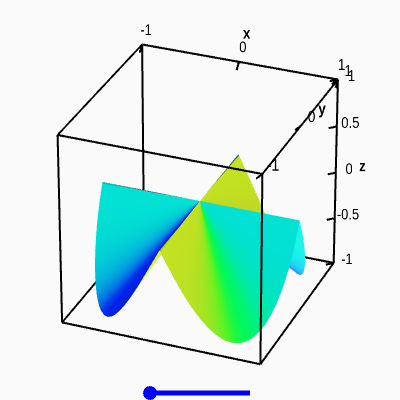
\includegraphics[width=.5\textwidth]{2-Differentiabilite-A}
  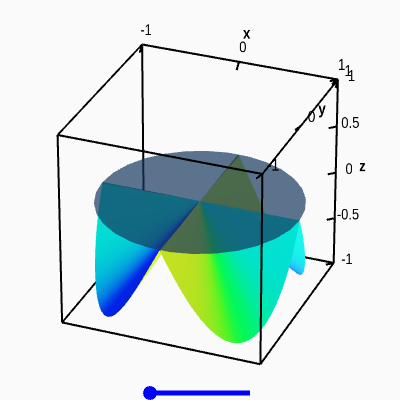
\includegraphics[width=.5\textwidth]{2-Differentiabilite-B}
  $$
  source: \url{https://mathinsight.org/differentiability_multivariable_subtleties}
  }
  \item Dans le cas de la fonction
  $$
  \begin{array}{rrcl}
    f : & \Rbb^n & \mapsto & \Rbb \\
    & x & \to & x^\top B x
  \end{array}
  $$
  on a donc montré que $J_x f = x^\top (B + B^\top)$. Dans le cas ou $B$ est symétrique, on obtient $J_x f = 2 x^\top B$ où l'on retrouve la forme de la dérivée de $bx^2$, à savoir $2 bx$.

\end{enumerate}

% \progres{
%   Rappel cours 3:
%   \begin{enumerate}
%     \item Normes et équivalence de normes en dimension finie
%     \item Différentiabilité 
%     \begin{itemize}
%      \item Application linéaire tangente
%      \item Matrice jacobienne
%     \end{itemize}
%   \end{enumerate}
%   Début cours 4. 
%   \begin{enumerate}
%     \item Différentiabilité
%     \begin{itemize}
%      \item Plan tangent, coordonnées polaires
%      \item Composition
%      \item Fonction implicite
%     \end{itemize}
%     \item Intégrales
%     \item Extremums
%   \end{enumerate}
% }

%-------------------------------------------------------------------------------
\subsubsection*{Plan tangent ($n = 2, k = 2$)}
%-------------------------------------------------------------------------------

La propriété \ref{prop:matriceJacobienne} justifie l'intérêt de la matrice jacobienne pour approcher les variations de l'application $f$ autour du point $x$ par une application linéaire : 
$$
f(x+h) - f(x) = J_xf \cdot h + o(\|h\|).
$$

Notamment, pour un fonction $f : \Rbb^2 \mapsto \Rbb$, on peut déterminer ainsi le plan tangent à une surface $S$ de $\Rbb^3$ d'équation
$$
z = f(x, y).
$$
au point $(x_0, y_0)$ pour peu que $f$ soit différentiable en $(x, y)$. Pour cela, on pose $z_0 = f(x_0, y_0)$ et $h = (x-x_0, y-y_0)$, qui donne
$$
f(x, y) - f(x_0, x_0) = \left(J_{(x_0, y_0)} f\right) \; h + o(\|h\|).
$$
Le plan tangent a ainsi pour équation
$$
z = z_0 + \frac{\partial f}{\partial x}(x_0, y_0) \times (x-x_0) + \frac{\partial f}{\partial y}(x_0, y_0) \times (y-y_0).
$$

\exemple{
Pour
$$
f(x, y) = \exp\left(-\frac{x^2 + y^2}{2}\right),
$$
on a 
$$
\frac{\partial f}{\partial x}(x_0, y_0) = - x_0 f(x_0, y_0), 
\qquad
\frac{\partial f}{\partial y}(x_0, y_0) = - y_0 f(x_0, y_0)
$$
et le plan tangent a pour équation
$$
z 
= f(x_0, y_0)(1 - x_0 (x-x_0) - y_0 (y-y_0))
= f(x_0, y_0)(1 + x_0^2 + y_0^2 - x_0 x - y_0 y)
$$
Ce plan est bien horizontal pour $(x_0, y_0) = (0, 0)$.
}

%-------------------------------------------------------------------------------
\exemple{
Soit 
$$
\begin{array}{rrcl}
  f : & \Mcal_n(\Rbb) & \mapsto & \Rbb \\
  & X & \to & \log(|X|)
\end{array}
$$
On remarque tout d'abord que $f$ n'est définie que pour les matrices $X$ inversibles dont le déterminant est (strictement) positif : $|X| > 0$. \\
On cherche à déterminer la matrice de ses dérivées partielles :
$$
D_X = [d_{X, ij}]: \qquad d_{X, ij} = \left.\frac{\partial f}{\partial x_{ij}}\right|_X.
$$
On remarque tout d'abord que 
$$
\frac{\partial \log(|X|)}{\partial x_{ij}}
= \frac1{|X|} \frac{\partial |X|}{\partial x_{ij}}.
$$
Pour calculer la dérivée de $|X|$ par rapport à $x_{ij}$, on utilise le développement par rapport à la $i$-ème ligne : 
$$
|X| = \sum_{j=1}^n x_{ij} (-1)^{i+j} |X^{i, j}|, 
$$
soit
$$
\frac{\partial |X|}{\partial x_{ij}} = (-1)^{i+j} |X^{i, j}|
$$
où on reconnaît le cofacteur de $x_{ij}$. On a donc 
$$
d_{X, ij} = \frac1{|X|} (-1)^{i+j} |X^{i, j}| 
\qquad \Rightarrow  \qquad
D_X = \frac1{|X|} \left[(-1)^{i+j} |X^{i, j}|\right]
$$
où on reconnaît la transposée de l'inverse de $X$ : 
$$
D_X = (X^{-1})^\top.
$$
On a donc
$$
\log(|X + H|) = \log(|X|) + \sum_{i, j} [(X^{-1})^\top H]_{i, j} + o(\|H\|).
$$
}

%-------------------------------------------------------------------------------
\subsubsection*{Transformation en coordonnées polaires} 
%-------------------------------------------------------------------------------

\begin{proposition} \label{prop:differentiabiliteCoordonneesPolaires}
  La transformation des coordonnées polaires en coordonnées cartésiennes 
  $$
  \begin{array}{rrcl}
    f : & \Rbb^+ \times [0, 2\pi] & \mapsto & \Rbb^2 \\
    & (\rho, \theta) & \to & (x = \rho \cos \theta, y = \rho \sin \theta).
  \end{array}
  $$
  est partout différentiable sur $\Rbb^{*+} \times \Rbb^+$.
\end{proposition}

% {Démonstration de la proposition \ref{prop:differentiabiliteCoordonneesPolaires}.}
\proof
Pour $u = [\rho \; \theta]^\top$ et $h = [r \; t ]^\top$, on a
$$
f(u+h) = \left[\begin{array}{c} 
    (\rho+r) \cos(\theta +t) \\ (\rho+r) \sin(\theta +t) 
    \end{array} \right]
$$
or, les fonctions cosinus et sinus sont partout dérivables et on a pour tout $\theta$
$$
\cos(\theta +t) = \cos \theta - t \sin \theta + o(|t|), \qquad 
\sin(\theta +t) = \sin \theta + t \cos \theta + o(|t|),
$$
donc
\begin{align*}
  (\rho+r) \cos(\theta +t) 
    & = (\rho+r)\left(\cos \theta - t \sin \theta + o(|t|)\right) \\
    & = \rho \cos \theta - \left(\rho t \sin \theta + r \cos \theta\right)
    - rt \sin \theta + (\rho + r) o(|t|),
\end{align*}
et de même pour $(\rho+r) \sin(\theta +t)$.
On a donc
\begin{align*}
  f(u+h) 
  & =
  \underset{f(u)}{\underbrace{\left[\begin{array}{c}
    \rho \cos \theta \\ \rho \sin \theta
  \end{array} \right]}}
  +
  \underset{D_u f \cdot h}{\underbrace{\left[\begin{array}{rr} 
          \cos \theta & - \rho \sin \theta \\
          \sin \theta & \rho \cos \theta 
        \end{array} \right]
  \left[\begin{array}{c} r \\ t \end{array} \right]}}
  +
  \underset{\text{reste}}{\underbrace{\left[\begin{array}{r} 
          - rt \sin \theta + (\rho + r) o(|t|) \\
          rt \cos \theta + (\rho + r) o(|t|) 
        \end{array} \right]}}.
\end{align*}
Il reste à montrer que le reste est un $o(\|h\|)$. 
\begin{itemize}
  \item En prenant $\|h\| = \|h\|_\infty = \max(|r|, |t|)$, on a clairement $|t| \leq \|h\|$, donc $o(|t|) = o(\|h\|)$. 
  \item De plus
  $$
  \left|\frac{rt}{\|h\|}\right| 
  \leq \frac{\|h\|^2}{\|h\|}
  \qquad \Rightarrow \qquad 
  rt = o(\|h\|).
  $$
  $rt \sin \theta$ et $rt \cos \theta$ sont donc des $o(\|h\|)$, 
\end{itemize}
Le vecteur reste est donc un $o(\|h\|)$.
\eproof

\remarks
\begin{itemize}
  \item La matrice jacobienne de cette transformation est
  $$
  J_{(\rho, \theta)}f = \left[ \begin{array}{rclcrcl}
      \frac{\partial}{\partial \rho} \rho \cos \theta & = & \cos \theta  & &
      \frac{\partial}{\partial \theta} \rho \cos \theta & = & -\rho \sin \theta  \\
      \frac{\partial}{\partial \rho} \rho \sin \theta & = & \sin \theta  & & 
      \frac{\partial}{\partial \theta} \rho \sin \theta & = & \rho \cos \theta  
    \end{array} \right].
  $$
  \item On peut remarquer que
  $$
  |J_{(\rho, \theta)}f| 
  = \left| \begin{array}{cc}
      \cos \theta  & -\rho \sin \theta  \\
      \sin \theta  & \rho \cos \theta  
    \end{array} \right|
  = \rho \cos^2\theta + \rho \sin^2 \theta = \rho.
  $$
\end{itemize}


%-------------------------------------------------------------------------------
%-------------------------------------------------------------------------------
\subsection{Composition} 
%-------------------------------------------------------------------------------

On cherche maintenant à généraliser la formule connue pour deux applications $f$ et $g$ de $\Rbb$ dans $\Rbb$:
$$
(f \circ g)'(x) = g'(x) (f' \circ g)(x).
$$

\begin{proposition} \label{prop:compositionDifferentielles}
  Si $g : \Rbb^n \mapsto \Rbb^k$ est différentiable en $x$ et $f : \Rbb^k \mapsto \Rbb^\ell$ est différentiable en $g(x)$, alors
  \begin{itemize}
   \item $f \circ g: \Rbb^n \mapsto \Rbb^\ell$ est différentiable en $x$ et
   \item sa différentielle vaut
   $$
   D_x(f \circ g) = D_{g(x)}f \circ D_xg
   $$
   et donc
   $$
   J_x(f \circ g) = J_{g(x)}f \cdot J_xg.
   $$
  \end{itemize}
\end{proposition}

\proof Cette proposition n'est pas démontrée ici. \eproof

%-------------------------------------------------------------------------------
\exemple{
Soient $f : \Rbb^k \mapsto \Rbb$ et $g : \Rbb \mapsto \Rbb^k$ telle que $g$ est différentiable en $x^*$ et $f$ en $g(x^*)$, on a
$$
J_{y^*}f = \left[\left.\frac{\partial f}{\partial y_1}\right|_{y^*} 
  \cdots 
  \left.\frac{\partial f}{\partial y_k}\right|_{y^*}  \right] 
\qquad \text{et} \qquad 
J_{x^*}g = \left[\begin{array}{c}
              \displaystyle{\left.\frac{\partial g_1}{\partial x}\right|_{x^*}}  \\
              \vdots \\
              \displaystyle{\left.\frac{\partial g_k}{\partial x}\right|_{x^*}} 
             \end{array}\right]
        = \left[\begin{array}{c} g'_1(x^*) \\ \vdots \\ g'_k(x^*) \end{array}\right]
$$
donc
$$
J_{x^*}(f \circ g) 
  = J_{g(x^*)} f \cdot J_{x^*}g
  = \left[\left.\frac{\partial f}{\partial y_1}\right|_{g(x^*)} 
    \cdots 
    \left.\frac{\partial f}{\partial y_k}\right|_{y^*}  \right] 
    \left[\begin{array}{c} g'_1(x^*) \\ \vdots \\ g'_k(x^*) \end{array}\right] 
  = \sum_{i=1}^k \left.\frac{\partial f}{\partial y_i}\right|_{g(x^*)} g'_i(x^*).
$$
}

\exemple{
  Soit une courbe exprimée en coordonnées polaires $\rho = \rho(\theta)$. 
  On peut déterminer les dérivées des coordonnées cartésiennes $x$ et $y$ par rapport à $\theta$ en considérant les deux applications 
  $$
  \begin{array}{rrcl}
    g : & \Rbb^+ & \mapsto & \Rbb^+ \times \Rbb^+ \\
    & \theta & \to & g(\theta) = (\rho(\theta), \theta)
  \end{array}
  $$
  et
  $$
  \begin{array}{rrcl}
    f : & \Rbb^+ \times \Rbb^+ & \mapsto & \Rbb^2 \\
    & (\rho, \theta) & \to & f(\rho, \theta) = (x = \rho \cos \theta, y = \rho \sin \theta).
  \end{array}
  $$
  On a
  $$
  J_{(\rho, \theta)}f = \left[ \begin{array}{ccc}
      \cos \theta  & & -\rho \sin \theta  \\
      \sin \theta  & & \rho \cos \theta  
    \end{array} \right]
  \text{ (déjà vu)}
  \qquad \text{et} \qquad 
  J_\theta g = \left[\begin{array}{c} \rho'(\theta) \\ 1 \end{array} \right].
  $$
  On a donc
  $$
  J_{\theta}(f \circ g) 
  = J_{(\rho(\theta), \theta)}f \cdot J_\theta g
  = \left[ \begin{array}{ccc}
      \cos \theta  & & -\rho(\theta) \sin \theta  \\
      \sin \theta  & & \rho(\theta) \cos \theta  
    \end{array} \right]
    \cdot
    \left[\begin{array}{c} \rho'(\theta) \\ 1 \end{array} \right]
  = \left[ \begin{array}{c}
      \rho'(\theta) \cos \theta  - \rho(\theta) \sin \theta  \\
      \rho'(\theta) \sin \theta  + \rho(\theta) \cos \theta  
    \end{array} \right],
  $$
  c'est-à-dire
  $$
  x'(\theta) = \frac{\partial x}{\partial \theta} = \rho'(\theta) \cos \theta  - \rho(\theta) \sin \theta, \qquad 
  y'(\theta) = \frac{\partial y}{\partial \theta} = \rho'(\theta) \sin \theta  + \rho(\theta) \cos \theta.
  $$
  On peut d'ailleurs retrouver
}

\exemple{
  [Cas de la spirale linéaire : $\rho(\theta) = b \theta$.]
  $$
  \begin{tabular}{ccc}
    $(x(\theta), y(\theta))$ & $(\theta, x(\theta))$ & $(\theta, y(\theta))$ \\
    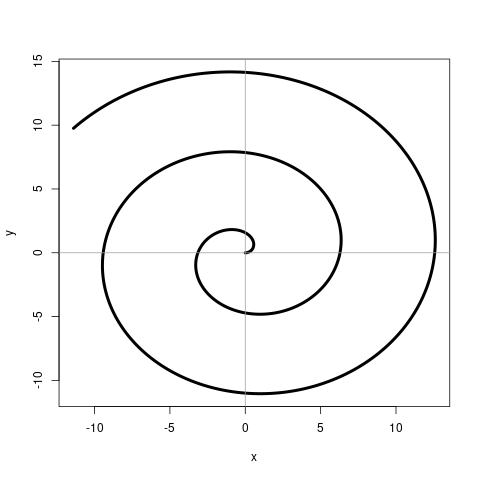
\includegraphics[width=.3\textwidth, trim=0 10 20 30, clip=]{Spirale-XY} & 
    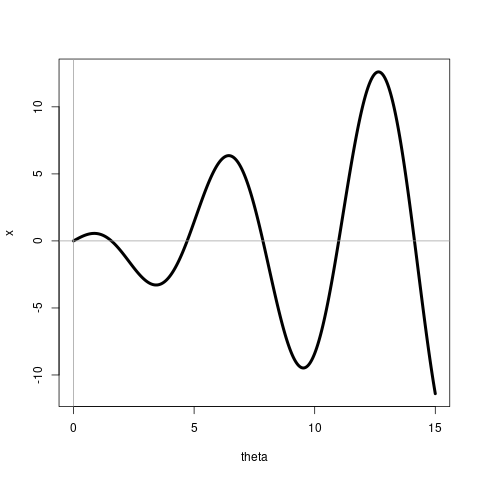
\includegraphics[width=.3\textwidth, trim=0 10 20 30, clip=]{Spirale-thetaX} & 
    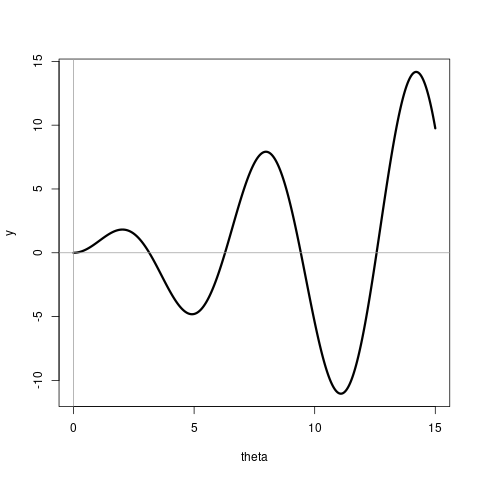
\includegraphics[width=.3\textwidth, trim=0 10 20 30, clip=]{Spirale-thetaY} 
  \end{tabular}
  $$
}

%-------------------------------------------------------------------------------
%-------------------------------------------------------------------------------
\subsection{Fonction implicite}
%-------------------------------------------------------------------------------

\begin{theorem}[Fonction implicite] \label{thm:fonctionImplicite}
  Soient $f : \Rbb^2 \mapsto \Rbb$ continuement différentiable, $\Ccal_z$ la courbe de niveau $z$ de $f$ :
  $$
  \Ccal_z = \{x, y: f(x, y) = z\},
  $$
  et $(x_0, y_0) \in \Rbb^2$ tels que 
  $$
  \left.\frac{\partial f}{\partial y}\right|_{x_0, y_0} \neq 0,
  $$
  il existe un voisinage $U \times V$ de $(x_0, y_0)$ et une application $\phi : \Rbb \mapsto \Rbb$ différentiable tels que, pour tout $(x, y) \in U \times V$
  $$
  (x, y) \in \Ccal \quad \Leftrightarrow \quad y = \phi(x).
  $$
  De plus
  $$
  \phi'(x_0) = - \left( \left. \frac{\partial f}{\partial x}\right|_{x_0, \phi(x_0)} \right) \left/ \left( \left. \frac{\partial f}{\partial y}\right|_{x_0, \phi(x_0)} \right. \right).
  $$
\end{theorem}

$$
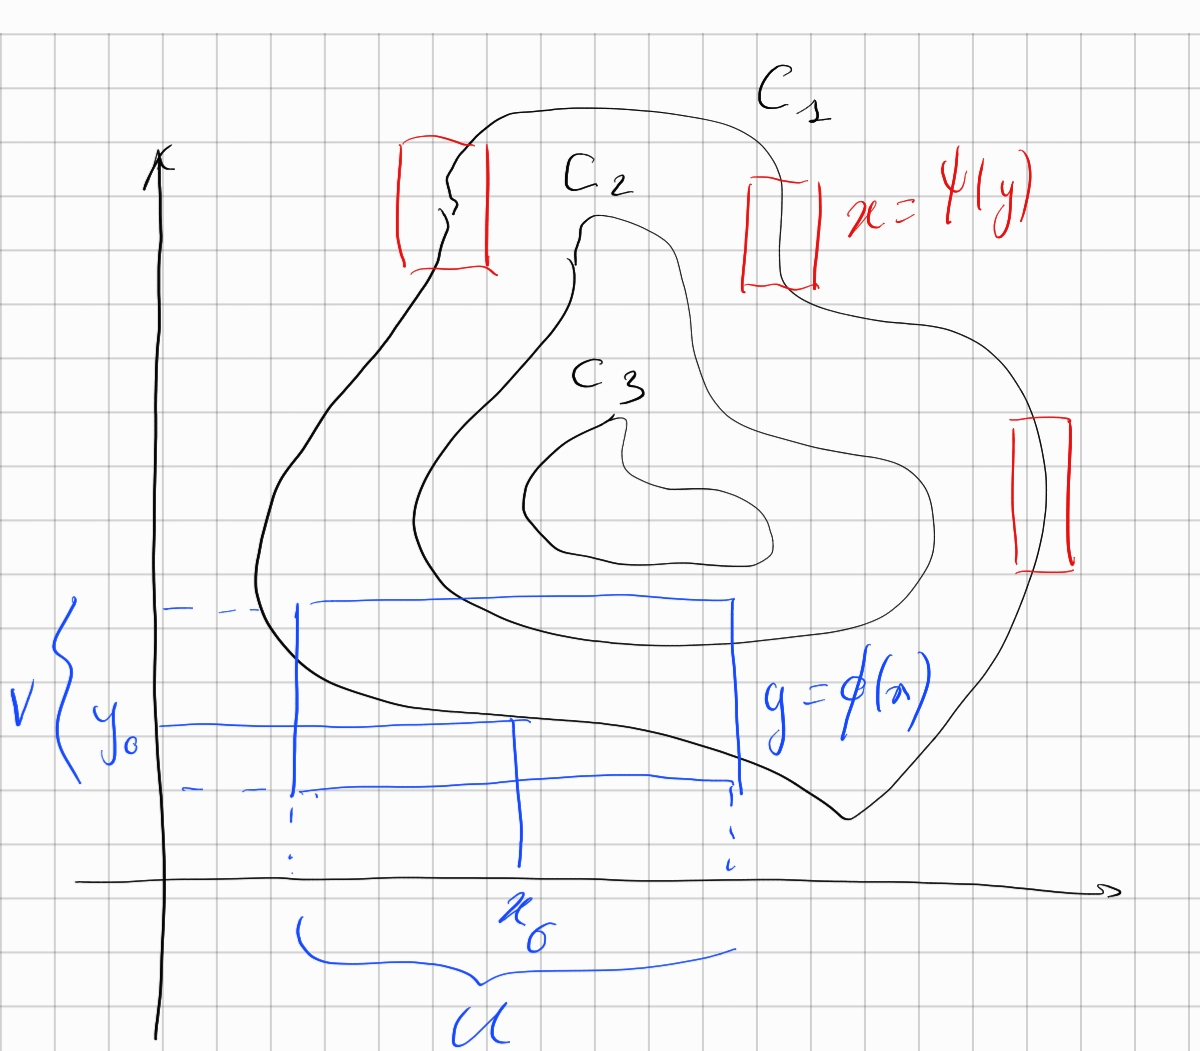
\includegraphics[width=.6\textwidth]{FonctionImplicite}
$$

% {Démonstration partielle du théorème \ref{thm:fonctionImplicite}.}
\proof [partielle]
On ne démontre pas ici l'existence de $\phi$. Par contre, la détermination de sa dérivée résulte d'un calcul simple. Pour cela, on définit
$$
\begin{array}{rrcl}
  g : & \Rbb & \mapsto & \Rbb^2 \\
  & x & \to & \left[\begin{array}{c} x \\ \phi(x) \end{array}\right]
\end{array}
$$
pour laquelle on a
$$
J_x g = \left[\begin{array}{c} 1 \\ \phi'(x) \end{array}\right]
$$
On a alors $f(x, \phi(x))= f \circ g (x)$ et donc
$$
(f \circ g)'(x_0) 
= J_{g(x_0)}f \;.\; J_{x_0}g
= \left( \left. \frac{\partial f}{\partial x}\right|_{x_0, \phi(x_0)} \right) + \phi'(x) \left( \left. \frac{\partial f}{\partial y}\right|_{x_0, \phi(x_0)} \right).
$$
Or, le long de la courbe de niveau $\Ccal_z$, on a $f(x, \phi(x)) \equiv z$, soit $(f \circ g)'(x) = 0$. On a donc
$$
\phi'(x_0) = - \left( \left. \frac{\partial f}{\partial x}\right|_{x_0, \phi(x_0)} \right) \left/ \left( \left. \frac{\partial f}{\partial y}\right|_{x_0, \phi(x_0)} \right. \right).
$$
\eproof

\exemple{\textcolor{gray}{
  Soit une courbe exprimée en coordonnées polaires $\rho = \rho(\theta)$. 
  La pente de la tangente à la courbe paramétrée $(x(\theta), y(\theta))$ s'obtient comme le rapport des dérivées partielles soit
  $$
  \frac{y'(\theta)}{x'(\theta)} 
  = \frac{\rho'(\theta) \sin \theta  + \rho(\theta) \cos \theta}{\rho'(\theta) \cos \theta  - \rho(\theta) \sin \theta}. 
  $$
}}

%-------------------------------------------------------------------------------
\exemple{\textcolor{gray}{[Cas de la spirale.]
  La spirale ``linéaire'' est définie par l'équation
  $$
  \rho(\theta) = \rho_0 \theta
  \qquad \Rightarrow \qquad
  \rho'(\theta) = \rho_0,
  $$
  pour laquelle on obtient
  $$
  x'(\theta) = \rho_0 \cos \theta - \rho_0 \theta \sin \theta, \qquad 
  y'(\theta) = \rho_0 \sin \theta + \rho_0 \theta \cos \theta
  $$
  soit une pente de 
  $$
  \frac{y'(\theta)}{x'(\theta)} = \frac{\sin \theta + \theta \cos \theta}{\cos \theta - \theta \sin \theta}.
  $$
  Pour la spirale logarithmique
  $$
  \rho(\theta) = a b^\theta
  \qquad \Rightarrow \qquad
  \rho'(\theta) = a b^\theta \log b,
  $$
  on obtient
  $$
  x'(\theta) = a b^\theta \log b \cos \theta - a b^\theta \sin \theta, \qquad 
  y'(\theta) = a b^\theta \log b \sin \theta + a b^\theta \cos \theta.
  $$
  soit une pente de 
  $$
  \frac{y'(\theta)}{x'(\theta)} = \frac{\log b \sin \theta + \cos \theta}{\log b \cos \theta - \sin \theta}.
  $$
  % Pour 
  % $$
  % \rho(\theta) = \rho_0 \log(\theta)
  % \qquad \Rightarrow \qquad
  % \rho'(\theta) = \rho_0 / \theta,
  % $$
  % on obtient
  % $$
  % x'(\theta) = \frac{\rho_0 \cos \theta}{\theta} - \rho_0 \log(\theta) \sin \theta, \qquad 
  % y'(\theta) = \frac{\rho_0 \sin \theta}{\theta} + \rho_0 \log(\theta) \cos \theta.
  % $$
}}


\newpage %-------------------------------------------------------------------------------
%-------------------------------------------------------------------------------
\section{Intégrales}
%-------------------------------------------------------------------------------

% Jacobien et changement de variables en dimension supérieure ou égale à 2.

% \begin{theorem}{Fubini-Tonelli}
% \end{theorem}
% 
% \begin{theorem}{Fubini-Lebesque}
% \end{theorem}

%-------------------------------------------------------------------------------
\subsection{Difféomorphisme}
%-------------------------------------------------------------------------------

\begin{definition}[Difféomorphisme]
  Soient $\Xcal$ et $\Ycal$ deux ouverts de $\Rbb^n$ et une bijection $g : \Xcal \mapsto \Ycal$. $g$ est un difféomorphisme si $g$ est différentiable partout dans $\Xcal$ et que $g^{-1}$ est différentiable partout dans $\Ycal$. \\
  Si, de plus, les dérivées partielles de $g$ et $g^{-1}$ sont partout continues, $g$ est un $C^1$-difféomorphisme.
\end{definition}

%-------------------------------------------------------------------------------
\paragraph*{Différentielle de la réciproque.}
Si $g : \Xcal \mapsto \Ycal$ est un difféomorphisme, puisque $g^{-1} \circ g = Id$ et que $D_x Id = I_n$, on a
$$
I_n = D_x(g^{-1} \circ g) = D_{g(x)}(g^{-1}) D_x g 
\qquad \text{(par composition)},
$$
soit
$$
D_{g(x)}g^{-1} = (D_x g)^{-1}.
$$
On retrouve ainsi la formule valable dans $\Rbb$ :
$$
(g^{-1})'(y) = 1 /g'(x)
\qquad \text{ou} \quad x = g^{-1}(y).
$$

\begin{theorem}[Inversion globale]
  Soit $\Xcal$ un ouvert de $\Rbb^n$ et $g : \Xcal \mapsto \Rbb^n$. Supposons que $g$ est injective, différentiable sur tout $\Xcal$ et que ses dérivées partielles sont partout continues dans $\Xcal$. Si, de plus, $D_x g$ est inversible sur tout $\Xcal$, alors $g : \Xcal \mapsto \Ycal = g(\Xcal)$ est un $C^1$-difféomorphisme.
\end{theorem}

\proof Non démontré. \eproof

\remark
Ce théorème assure le $C^1$-difféomorphisme sans exiger la différentiabilité continue de $g^{-1}$.

%-------------------------------------------------------------------------------
\subsection{Jacobien, changement de variable}
%-------------------------------------------------------------------------------

\begin{definition}[Jacobien]
  Pour $g : \Rbb^n \mapsto \Rbb^n$, le jacobien de $f$ au point $x$ est le déterminant de sa matrice jacobienne au point $x$ : 
  $$
  |J_x f|.
  $$
\end{definition}

\remark
Le jacobien d'un difféomorphisme ne peut pas être nul, puisqu'un difféomorphisme est bijectif :
$$
|J_x f| \neq 0.
$$

\begin{theorem}[Changement de variable]
  Soit $\Xcal$ et $\Ycal$ deux ouverts de $\Rbb^n$ et $g : \Xcal \mapsto \Ycal = g(\Xcal)$ un $C^1$-difféomorphisme et $f : \Ycal \mapsto \Rbb^+$, on a 
  $$
  \int_\Ycal f(y) \; \d y = \int_\Xcal f \circ g(x) |J_x g| \; \d x.
  $$
\end{theorem}

\proof
Non démontrée.
% : la preuve passe par le découpage du domaine d'intégration en fonction des différents type d'action de la matrice jacobienne $J_x g$ (transvection, permutation ou dilatation).
\eproof

%-------------------------------------------------------------------------------
\textcolor{gray}{\remark
La contrainte de signe pour $f$ assure que le résultat de l'intégration ne dépend pas de l'ordre selon lequel on intègre par rapport aux différente coordonnée (théorème Fubini-Tonelli). Le théorème de Fubini-Lebesgue lève cette contrainte mais requiert que $f$ soit bornée.}

%-------------------------------------------------------------------------------
\begin{corollary*}[Coordonnées polaires]
  Pour tout $f : \Rbb^2 \mapsto \Rbb^+$, 
  $$
  \int_\Rbb \int_\Rbb f(x, y) \; \d x \d y
  = \int_{\Rbb^+} \int_0^{2 \pi} f(\rho \cos \theta, \rho \sin \theta) \rho \; \d \rho \d \theta
  $$
\end{corollary*}

\proof
\begin{itemize}
  \item On a vu que la transformation en coordonnées polaires $g$ est partout différentiable et que $|J_{(\rho, \theta)}g| = \rho$.
  \item On vérifie facilement que $g$ est bijective et que ses dérivées partielles sont partout continues.
\end{itemize}
\eproof

%-------------------------------------------------------------------------------
\exemple{
  Pour calculer 
  $$
  I = \int_\Rbb e^{-x^2} \; \d x,
  $$
  on peut passer en coordonnées polaires pour calculer
  \begin{align*}
  J 
  & = \int_\Rbb \int_\Rbb e^{-(x^2+y^2)} \; \d x \; \d y
  = \int_{\Rbb^+} \int_0^{2 \pi} e^{-\rho^2} \rho \; \d \rho \; \d \theta \\
  & = \int_{\Rbb^+} e^{-\rho^2} \rho \; \d \rho \times \int_0^{2 \pi} \d \theta 
  = \left[-\frac12 e^{-\rho^2}\right]_0^\infty \times 2 \pi \\
  & = \pi
  \end{align*}
  puis remarquer que $J = I^2$ pour conclure que $I = \sqrt{\pi}$.
}

\remark
Par le le même calcul, on montre que $\int_\Rbb e^{-x^2/2} \; \d x = \sqrt{2 \pi}$, ce qui justifie la constante de normalisation de la densité de la loi normale d'espérance nulle et de variance 1 : 
$$
\phi(x) = \frac1{\sqrt{2\pi}} \exp(- x^2/2).
$$

%-------------------------------------------------------------------------------
%-------------------------------------------------------------------------------
\section{Extremums}
%-------------------------------------------------------------------------------

%-------------------------------------------------------------------------------
\subsection{\textcolor{gray}{Variétés}}
%-------------------------------------------------------------------------------

\textcolor{gray}{Courbe de niveau (cf notes manuscrites, dans section chgt de variable)}

%-------------------------------------------------------------------------------
\subsection{Extrema}
%-------------------------------------------------------------------------------

\begin{definition}[Gradient]
  Soit $f : \Rbb^k \mapsto \Rbb$ différentiable en $x^*$, le gradient de $f$ en $x^*$ est le vecteur constitué de ses dérivées partielles évaluées en $x^*$ : 
  $$
  \nabla_{x^*}f 
  = \left[\begin{array}{c}
              \displaystyle{\left.\frac{\partial f}{\partial x_1}\right|_{x^*}}  \\
              \vdots \\
              \displaystyle{\left.\frac{\partial f}{\partial x_k}\right|_{x^*}} 
             \end{array}\right]
  = \left[J_{x^*} f\right]^\top.
  $$
\end{definition}

%-------------------------------------------------------------------------------
\remark
\begin{enumerate}
  \item Si $f$ est différentiable en $x$, on a
  $$
  f(x + h) = f(x) + \nabla_{x^*}f^\top h + o(\|h\|).
  $$
  \item Un point $x$ pour lequel le gradient de $f$ est nul est appelé {\em point stationnaire} (ou {\em point critique}) de $f$ : au premier ordre, la fonction $f$ est constante au voisinage de $x$.
\end{enumerate}


%-------------------------------------------------------------------------------
\begin{definition}[Matrice hessienne]
  Soit $f : \Rbb^n \mapsto \Rbb$ différentiable en $x^*$, la matrice hessienne ('la hessienne') $f$ en $x^*$ est la matrice ayant pour éléments génériques les dérivées secondes croisées évaluées en $x^*$ : 
  $$
  \nabla^2_{x^*}f 
  = \left[\left.\frac{\partial^2 f}{\partial x_i\partial x_j}\right|_{x^*} \right]_{1 \leq i, j \leq n}
%   = \left[\begin{array}{ccc}
%               \displaystyle{\left.\frac{\partial^2 f}{\partial x_1^2}\right|_{x^*}} & 
%               \cdots & 
%               \displaystyle{\left.\frac{\partial^2 f}{\partial x_1\partial x_k}\right|_{x^*}} \\
%               \vdots & 
%               \displaystyle{\left.\frac{\partial^2 f}{\partial x_i\partial x_j}\right|_{x^*}}\vdots & 
%               \\
%               \displaystyle{\left.\frac{\partial^2 f}{\partial x_k\partial x_1}\right|_{x^*}} & 
%               \cdots & 
%               \displaystyle{\left.\frac{\partial^2 f}{\partial x_k^2}\right|_{x^*}}
%           \end{array} \right].
  $$
  Les termes diagonaux de $\nabla^2_{x^*}f$ sont les dérivées secondes par rapport à chacune des coordonnées : 
  $$
  \left[ \nabla^2_{x^*}f \right]_{ii} 
  = \left.\frac{\partial^2 f}{\partial x_i^2}\right|_{x^*}.
  $$
  Notamment, si $f$ est $C^2$, $\nabla^2_{x^*}f$ est symétrique (car on peut alors inverser l'ordre des dérivées), ce qui implique qu'elle est diagonalisable.
\end{definition}

%-------------------------------------------------------------------------------
\begin{proposition} \label{prop:taylorOrdre2}
  Si $f$ est deux fois différentiable en $x$, alors
  $$
  f(x+h) = f(x) + \nabla_x f^\top \cdot h + \frac12 h^\top \cdot \nabla^2_x f \cdot h + o(\|h\|^2).
  $$
\end{proposition}

% {Démonstration de la proposition \ref{prop:taylorOrdre2}.}
\proof
  Pour alléger les notations, on note ici
  $$
  f'_i(x^*) = \left. \frac{\partial f}{\partial x_i}\right|_{x^*}, \qquad 
  f''_{ij}(x^*) = \left. \frac{\partial^2 f}{\partial x_i \partial x_j}\right|_{x^*}.
  $$
  La démonstration repose sur le développement de Taylor en 0 d'une fonction $\phi$ de $\Rbb$ dans $\Rbb$ deux fois différentiable qui vaut
  \begin{equation} \label{eq:taylor2phi}
  \phi(t) = \phi(0) + t \phi'(0) + \frac12 \phi''(0) + o(t^2).
  \end{equation}
  \begin{enumerate}
    \item On pose tout d'abord $h = t u$, où $u$ est un vecteur fixe et on définit la fonction 
    $$
      \begin{array}{rrcl}
        g : & \Rbb & \mapsto & \Rbb^n \\
        & t & \to & x + t u
      \end{array}
    $$
    qui vérifie
    $$
    J_t g = u.
    $$
    En posant $\phi = f \circ g$, on obtient ainsi
    $$
    f(x + h) = \phi(t).
    $$
    \item Il nous faut maintenant déterminer $\phi'(0)$ et $\phi''(0)$.
    \begin{description}
      \item[$\phi'(t)$:] on a
        $$
        \phi'(t) = J_t \phi 
        = J_{g(t)} f \cdot J_t g
        = \nabla_{g(t)}f^\top u
        = \sum_{i=1}^n u_i f'_i(g(t))
        $$
      \item[$\phi''(t)$:] on a
      $$
      \phi''(t) 
      = \frac{\partial}{\partial t} \phi'(t)
      = \sum_{i=1}^n u_i \frac{\partial}{\partial t} f'_i(g(t))
      $$
      puisque $u_i$ ne dépend pas de $t$. On remarque alors que
      $$
      J_x f_i' = [f''_{i1}(x) \; \dots \; f''_{in}(x)]
      $$
      donc
      $$
      \frac{\partial}{\partial t} f'_i(g(t)) 
      = J_{g(t)} f_i' \cdot J_t g
      = J_{g(t)} f_i' \cdot u
      = \sum_{j=1}^n u_j f''_{ij}(g(t)),
      $$
      soit
      $$
      \phi''(t) 
      = \sum_{i=1}^n u_i \sum_{j=1}^n u_j f''_{ij}(g(t))
      = u^\top \nabla_{g(t)} u.
      $$
    \end{description}
    En reportant dans l'équation \eqref{eq:taylor2phi}, on obtient
    \begin{align*}
      \phi(t) 
    %       & = \phi(0) + t \phi'(0) + \frac12 t^2 \phi''(0) + o(t^2) \\
      & = \phi(0) + t \nabla_{g(0)}f^\top u + \frac12 t^2 u^\top \nabla_{g(0)} u + o(t^2) \\
      & = \phi(0) + \nabla_{g(0)}f^\top h + \frac12 h^\top \nabla_{g(0)} h + o(t^2)
    \end{align*}
    car $h = tu$, soit, en utilisant $\phi(t) = f(x)$, $\phi(0) = f(x)$ et $g(0) = x$,
    $$
    f(x+h) 
    = f(x) + \nabla_{x}f^\top h + \frac12 h^\top \nabla_{x} h + o(t^2).
    $$
    \item Il reste à vérifier que $o(t^2) = o(\|h\|^2)$, ce qui est vrai car $\|h\|^2 = t^2 \|u\|^2$ et $\|u\|^2$ est constante.
  \end{enumerate}
\eproof

\remark
$f$ est deux fois différentiable en $x$ signifie que $f$ est différentiable en $x$ et que l'application $g$ de $\Rbb^k$ dans $\Rbb^k$ définie par $g(x) = \nabla_x f$ est elle-même différentiable en $x$.

\begin{definition}[Extremum local]
  Si $f$ est deux fois différentiable en $x$ et que son gradient y est nul : $\nabla_xf = 0$, alors
  \begin{itemize}
   \item $x$ est {\em maximum local} si $\nabla^2_x f$ est définie négative et
   \item $x$ est {\em minimum local} si $\nabla^2_x f$ est définie positive.
  \end{itemize}
  Dans les deux cas, $x$ est un {\em optimum relatif}.
\end{definition}

\remark
Puisque le gradient $\nabla_x f$ est nul, on a au voisinage de $x$ :
$$
f(x+h) - f(x) \simeq \frac12 h^\top \cdot \nabla^2_x f \cdot h.
$$
Un maximum (resp. minimum) se caractérise par le fait que la fonction $f$ diminue (resp. augmente) dans toutes les directions $h$. Le fait que $\nabla^2_x f$ soit définie négative (resp. positive) assure précisément que $f(x+h) - f(x)$ est négatif (resp. positif) dans tout le voisinage de $x$.

%-------------------------------------------------------------------------------
\subsection*{Cas de $f : \Rbb^2 \mapsto \Rbb$}
%-------------------------------------------------------------------------------

\begin{definition}[Notation de Monge]
  Pour $f : \Rbb^2 \mapsto \Rbb$, on note les dérivées au point $a = (x^*, y^*) \in \Rbb^2$
  \begin{align*}
    p & = \left.\frac{\partial f}{\partial x}\right|_a, &
    q & = \left.\frac{\partial f}{\partial y}\right|_a, &
    r & = \left.\frac{\partial^2 f}{\partial x^2}\right|_a, &
    s & = \left.\frac{\partial^2 f}{\partial x \partial y}\right|_a, &
    t & = \left.\frac{\partial^2 f}{\partial y^2}\right|_a
  \end{align*}
  c'est à dire
  $$
  \nabla_af = \left[\begin{array}{c} p \\ q \end{array} \right], 
  \qquad 
  \nabla^2_af = \left[\begin{array}{cc} r & s \\ s & t \end{array} \right].
  $$
\end{definition}

%-------------------------------------------------------------------------------
\paragraph*{Caractérisation des optimums.}
Toutes les valeurs propres d'une matrice définie positive ou négative sont de même signe. 
En dimension deux, cela signifie que leur produit (qui est égal au déterminant) est positif. Si le produit est positif, leur signe commun est donné par leur somme (qui est égale à la trace).

$a = (x^*, y^*)$ pour lequel $\nabla_a f = 0$ (i.e. $p = q = 0$) est donc
\begin{itemize}
  \item un optimum relatif de $f$ si 
  $$
  |\nabla^2_a f| = rt - s^2 > 0 ;
  $$
  \item un maximum relatif de $f$ si 
  $$
  |\nabla^2_a f| = rt - s^2 > 0 
  \qquad \text{et} \qquad
  \tr(\nabla^2_a f) = r + t < 0 ;
  $$
  \item un minimum relatif de $f$ si 
  $$
  |\nabla^2_a f| = rt - s^2 > 0 
  \qquad \text{et} \qquad
  \tr(\nabla^2_a f) = r + t > 0 ;
  $$
  \item un point selle de $f$ si 
  $$
  |\nabla^2_a f| = rt - s^2 < 0
  $$
  ($a$ est un maximum dans une direction et un minimum dans une autre).
\end{itemize}

% \progres{
%   Début Cours 7. Rappels :
%   \begin{enumerate}[\itemdot]
%     \item Changement de variables
%     $$
%     \int_{\Rbb^n} f(y) \; \d y = \int_{\Rbb^n} f \circ g (x) \; |J_x g| \; \d x
%     $$
%     $|J_x g| =$ jacobien de $g$ au point $x$.
%     \item Extrema
%     $$
%     f(x+h) = f(x) + (\nabla_x f)^\top h + \frac12 h^\top (\nabla^2_x f) h + o(\|h\|^2).
%     $$
%     $x =$ extremum local si $\nabla_x f = 0$, maximum si $\nabla^2_x f \preccurlyeq 0$, minimum si $\nabla^2_x f \succcurlyeq 0$.
%     \item Cas particulier $\Rbb^n = \Rbb^2$ : caractérisation des extrémum à partir du déterminant et de la trace de $\nabla^2_x f$.
%     \item Exercice maison.
%   \end{enumerate}
% }

\begin{exercise*}[A faire à la maison]
  Déterminer les points stationnaires de la fonction 
  $$
  f(x, y) = x^3 + y^3 - 3 xy
  $$
  déterminer s'il s'agit de maximums, de minimums ou de points selles.
\end{exercise*}

\solution{
  \begin{description}
    \item[Points critiques :] Le gradient de $f$ vaut
    $$
    \nabla f = \left[\begin{array}{c} 3x^2 - 3y \\ 3y^2 - 3x \end{array}\right]
    $$
    qui est nul aux points
    $$
    a = (0, 0) \qquad \text{et} \qquad b = (1, 1).
    $$
    De plus la hessienne vaut
    $$
    \nabla^2 f = \left[\begin{array}{rrr} 6x & & -3 \\ -3 & & 6y \end{array}\right].
    $$
    %
    \item[\'Etude du point $a$ :] on a 
    $$
    \nabla_a^2 f = \left[\begin{array}{rrr} 0 & & -3 \\ -3 & & 0 \end{array}\right]
    \qquad \Rightarrow \qquad 
    | \nabla_a^2 f | = -9 < 0
    $$
    donc $a$ est un point selle. Ses valeurs propres sont les racines de
    $$
    P(\lambda) = \left|\begin{array}{rrr} -\lambda & & -3 \\ -3 & & -\lambda \end{array}\right|
    = \lambda^2 - 9 
    \qquad \text{soit} \quad 
    \lambda = \pm 3.
    $$
    Tout vecteur propre associé à $\lambda = -3$ est solution de 
    $$
    \left\{\begin{array}{rcl} -3y & = & -3x \\-3x & = & -3y\end{array} \right.
    \qquad \Rightarrow \qquad 
    x = y
    \qquad \Rightarrow \qquad 
    \left[ \begin{array}{r} 1 \\ 1 \end{array} \right] \text{ est associé à $-3$}
    $$
    donc $a$ est un maximum dans la direction de la 1ère bissectrice. \\
    Tout vecteur propre associé à $\lambda = 3$ est solution de 
    $$
    \left\{\begin{array}{rcl} -3y & = & 3x \\-3x & = & 3y\end{array} \right.
    \qquad \Rightarrow \qquad 
    x = -y
    \qquad \Rightarrow \qquad 
    \left[ \begin{array}{r} -1 \\ 1 \end{array} \right] \text{ est associé à $+3$}
    $$
    donc $a$ est un minimum dans la direction de la 2ème bissectrice.
    %
    \item[\'Etude du point $b$ :] on a
    $$
    \nabla_b^2 f = \left[\begin{array}{rrr} 6 & & -3 \\ -3 & & 6 \end{array}\right]
    \qquad \Rightarrow \qquad 
    | \nabla_b^2 f | = 27 > 0, \qquad \tr(\nabla_b^2 f) = 12 > 0
    $$
    donc les deux valeurs propres de $\nabla_b^2 f$ sont positives : $b$ est donc un minimum.
  \end{description}
}

\dessin{
\paragraph*{Fonction $f(x, y) = x^3 + y^3 - 3xy$:}
$$
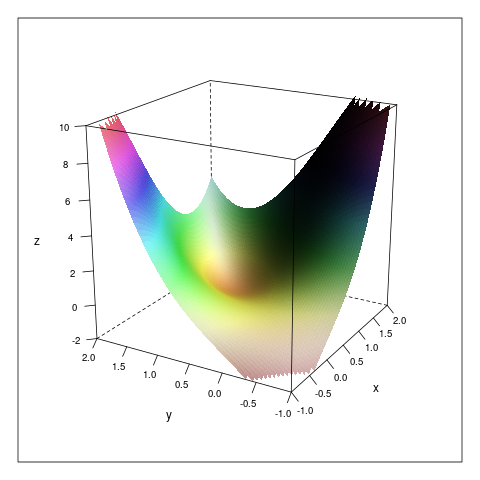
\includegraphics[width=.6\textwidth]{ExempleOptimum-surface}
$$
\paragraph*{Point $a = (0, 0)$:}
$$
\begin{tabular}{cc}
  direction $x = y$ & direction $x = -y$ \\
  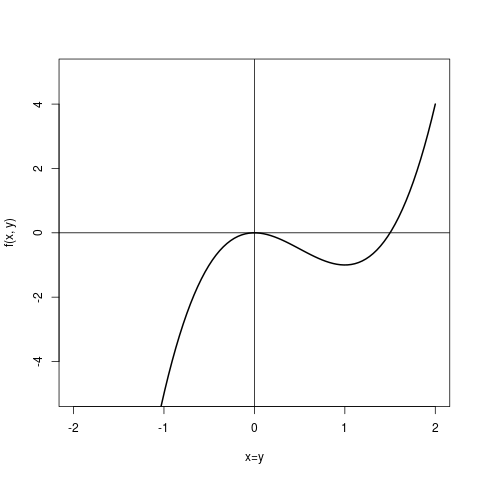
\includegraphics[width=.4\textwidth, trim=10 10 10 40, clip=]{ExempleOptimum-1ereBissectrice} &
  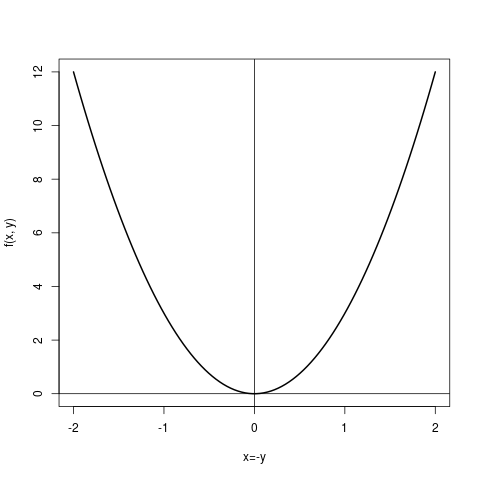
\includegraphics[width=.4\textwidth, trim=10 10 10 40, clip=]{ExempleOptimum-2emeBissectrice} \\
  $f(x, x) = 2x^3 - 3x^2$ & $f(x, -x) = 3x^2$
\end{tabular}
$$
}


%-------------------------------------------------------------------------------
\chapter{\'Equations différentielles et systèmes dynamiques}
\minitoc
%-------------------------------------------------------------------------------
\newpage % \'Equations différentielles et systèmes dynamiques en temps continu. Existence, unicité des solutions. Recherche des équilibres et linéarisation. Classification des équilibres en dimensions 1 et 2.

% \progres{
%   Rappel cours 4 :
%   \begin{itemize}
%     \item Différentiabilité, matrice jacobienne, composition
%     \item Intégration et changement de variable
%     \item Caractérisation des extremums
%     \item Exercice à faire : extrema de $f(x, y) = x^3 + y^3 - 3xy$.
%   \end{itemize}
%   Programme cours 5 :
%   \begin{itemize}
%     \item Chapitre 3 : équations différentielles et systèmes dynamiques
%     \item EDO en dimension 1 : solution maximale, stabilité
%     \item EDO en dimension $n$ : cas linéaire
%     \item EDO en dimension $n$ : cas non linéaire
%   \end{itemize}
% }

%-------------------------------------------------------------------------------
\paragraph*{Objectif.} 
On s'intéresse à une fonction 
$$
\begin{array}{rrcl}
  y : & \Rbb & \mapsto & \Rbb^n \\
  & t & \to & y(t) = [y_1(t) \dots y_n(t)]^\top 
\end{array}
$$
qui soit solution d'une équation {\em fonctionnelle} de la forme
$$
\nabla y(t) = F(y(t))
$$
où $F$ est une fonction de $\Rbb^n$ dans $\Rbb^n$. Une telle équation est appelée {\em équation différentielle ordinaire} (EDO, alias {\em ODE} en anglais).

Comme la notation le laisse entendre, la variable $t$ décrit typiquement un temps et $y(t)$ l'évolution d'un système à $n$ coordonnées au cours du temps partant d'une {\em condition initiale}
$$
y(t_0) = y_0.
$$
En notant $\dot y$ la dérivée de $y$ par rapport au temps, un tel {\em système dynamique} s'écrit donc
$$
\left\{\begin{array}{rcl}
        y(t_0) & = & y_0, \\
        \dot y & = & F(y).
       \end{array}\right.
$$

%-------------------------------------------------------------------------------
\paragraph*{Deux modèles classiques.}
\begin{description}
 \item[Lotka-Volterra:] $y(t) = [N(t) \; P(t)]^\top$ avec $N(t) =$ nombre de proies au temps $t$, $(t) = $ nombre prédateurs au temps $t$:
 $$
 \left\{ \begin{array}{rcl} 
  \dot N & = & r N - c N P \\
  \dot P & = & b N P  - m P
 \end{array} \right.
 $$
 La fonction $F$ est alors
 $$
 F\left(\begin{array}{c} y_1 \\ y_2 \end{array}\right) 
 = \left(\begin{array}{c} r y_1 - c y_1 y_2 \\ b y_1 y_2 - m y_2 \end{array}\right).
 $$
 \item[SIR :] $y(t) = [S(t) \; I(t) \; R(t)]^\top$ avec $S(t) =$ nombre de susceptibles au temps $t$, $I(t) =$ nombre d'infectés et $R(t) =$ nombre de 'remis' ({\em recovered}) :
 $$
 \left\{ \begin{array}{rcl} 
  \dot S & = & - r S I \\
  \dot I & = & r S I - a I \\
  \dot R & = & a I \\
 \end{array} \right.
 $$
 La fonction $F$ est alors
 $$
 F\left(\begin{array}{c} y_1 \\ y_2 \\ y_3 \end{array}\right) 
 = \left(\begin{array}{c} -r y_1 y_2 \\ r y_1 y_2 - a y_2 \\ a y_2 \end{array}\right).
 $$
 Un tel modèle est dit à compartiments, les compartiments étant les populations d'effectifs respectifs $S$, $I$ et $R$. 
\end{description}

Ces deux modèles sont fondés sur des sytèmes d'équations différentielles en dimension plus grande que 1 et non linéaires.

%-------------------------------------------------------------------------------
%-------------------------------------------------------------------------------
\section{Exemple en 1D et solution maximale, stabilité} \label{sec:EquaDiff-1DsolMaximale}
%-------------------------------------------------------------------------------

%-------------------------------------------------------------------------------
\paragraph*{ODE linéaire en dimension 1 : modèle de Malthus.}
L'EDO la plus simple en dimension 1 est l'équation linéaire
$$
\dot y = r y
$$
dont la solution est connue : 
$$
y(t) = a_0 e^{rt}.
$$
Le paramètre $a_0$ est alors déterminé par une condition 'initiale' : en imposant que $y(t_0) = y_0$, il vient
$$
a_0 = y_0 e^{-t_0} 
\qquad \Rightarrow \qquad
y(t) = y_0 e^{r(t-t_0)}.
$$
Ce modèle est connu en dynamique des population sous le nom de {\em modèle de Malthus} : il suppose que l'accroissement de la population est directement proportionnel à sa taille. Ce modèle n'inclue pas de limitation de la taille de la population et en prévoit donc une croissance indéfini pour $r > 0$ (et une extinction pour $r < 0$).


%-------------------------------------------------------------------------------
\subsection{Solution maximale} 
%-------------------------------------------------------------------------------

\begin{definition}[Solution du problème de Cauchy]
  Soit $F : \Rbb^n \mapsto \Rbb^n$, $I$ un ouvert de $\Rbb$, $t_0 \in I$ et $y_0 \in \Rbb$. La fonction $f : I \mapsto \Rbb^n$ est dite solution du \emph{problème de Cauchy}, 
  $$
  \left\{\begin{array}{rcl}
          y(t_0) & = & y_0, \\
          \dot y & = & F(y).
        \end{array}\right.
  $$
  sur $I$ si $f(t_0) = y_0$ et $\forall t \in I: \dot f(t) = F(f(t))$.
\end{definition}

\begin{theorem}[Cauchy-Lipschitz]
  Si $F$ est $C^1$ par morceaux, il existe une unique solution $f$ sur $I$ au problème de Cauchy qui soit maximale au sens où si $g$ est également solution sur $J$, alors $J \subset I$ et $g(t) = f(t)$ pour tout $t \in J$. $f$ est appelée solution maximale et $I$ intervalle maximal.
\end{theorem}

\proof Non démontré. \eproof

\remark
$f(t) = y_0 e^{r(t-t_0)}$ est donc l'unique solution du problème $\{y_0 = y(t_0), \; \dot y = r y\}$ sur l'intervalle maximal $\Rbb$.

%-------------------------------------------------------------------------------
\exemple{
  Pour déterminer la solution et l'intervalle maximal du problème
  $$
  \{y(0) = 1, \; \dot y = -c y^2\},
  $$
  on remarque que
  \begin{align*}
    \dot y & = -c y^2 & 
    & \Leftrightarrow & 
    c & = - \frac{\dot y}{y^2} = \frac{\partial}{\partial t} \frac1y = \dot{\left(\frac1y\right)}\\
    \text{donc} \qquad 
    \frac1y & = a + ct & 
    & \Leftrightarrow &
    y(t) & = \frac1{a + ct} \qquad \text{pour } t \neq -\frac{a}c.
  \end{align*}
  La condition $y(0) = 1$ impose alors que $a = 1$, soit 
  $$
  f(t) = (1+ ct)^{-1}
  $$ 
  est donc solution maximale sur l'intervalle (maximal) $\Rbb \setminus \{-1/c\}$.
}

%-------------------------------------------------------------------------------
\subsection{Point d'équilibre, stabilité} 
%-------------------------------------------------------------------------------

\begin{definition}[Point d'équilibre]
  $y^* \ \Rbb^n$ est un point d'équilibre de l'ODE $\dot y = F(y)$ si $F(y^*) = 0$.
\end{definition}

\begin{definition}[Stabilité ($n = 1$)]
  Pour $n = 1$, un équilibre $y^*$ est dit (asymptotiquement) stable si il existe $\varepsilon > 0$ tel que pour tout $y_0 \in (y^* - \varepsilon, y^* + \varepsilon)$, la condition initiale $y(0) = y_0$ implique que 
  $$
  \lim_{t \to \infty} y(t) = y^*.
  $$
  Dans le cas contraire, il est dit {\em instable}. Le caractère stable ou instable d'un équilibre définit sa {\em nature}.
\end{definition}

\remark
Un équilibre est donc stable si toute (petite) perturbation $\varepsilon$ autour de $y^*$ laisse le système retourner dans l'état $y^*$.


%-------------------------------------------------------------------------------
\paragraph*{Modèle de Verhulst.}
Une façon simple d'empêcher la croissance indéfinie de la population prédite par le modèle de Malthus consiste à supposer que le taux de reproduction $\dot y / y$ décroît linéairement avec la taille de la population : 
\begin{equation} \label{eq:verhulst}
\dot y / y = r - cy
\qquad \Leftrightarrow \qquad
\dot y = y(r - cy).
\end{equation}
Ce modèle est connu sous le nom de {\em modèle de Verhulst}. On suppose que les paramètres $r$ et $c$ sont positifs et on pose la condition initiale
$$
y(0) = y_0.
$$
\begin{description}
  \item[Points d'équilibre:] $y^* = 0$ et $y^* = K := r/c$ sont des points d'équilibre car alors $\dot y = F(y^*) = 0$.
  \item[Solution pour $y_0 \in \{0, K\}$:] la fonction $y(t)$ reste constante (car $\dot y(t) \equiv 0$).
  \item[Solution pour $0 < y_0 < K$:] on obtient une solution de cette équation en remarquant que
  $$
  r = \frac{\dot y}y + cy \qquad \Leftrightarrow \qquad y = \frac{\dot y}{r - cy},
  $$
  de plus, pour $t$ proche de 0, par continuité de $y$, on a $0 < y(t) < K$ et donc \eqref{eq:verhulst} est équivalente à 
  \begin{equation} \label{eq:verhulstSolution}
  r 
  = \frac{\dot y}{y} + \frac{c \dot y}{r - cy}
  = \frac{\partial}{\partial t} \left(\log y - \log (r - cy) \right)
  = \frac{\partial}{\partial t} \left(\log \left(\frac{y}{r - cy}\right)\right),
  \end{equation}
  soit
  $$  \log \left(\frac{y}{r - cy}\right) = rt + \log b
  \qquad \Leftrightarrow \qquad 
  \frac{y}{r - cy} = b e^{rt}
  \qquad \Leftrightarrow \qquad
  y(1 + c b e^{rt}) = r b e^{rt} \\
  $$
  soit encore
  \begin{equation} \label{eq:solutionVerhulst}
    y = \frac{rb e^{rt}}{1 + cb e^{rt}} = \frac{K a_0 e^{rt}}{1 + a_0 e^{rt}}
  \end{equation}
  avec $a_0 = cb > 0$.
  La forme de cette solution lui donne également le nom de modèle logistique. 
  
  On remarque que
  \begin{equation} \label{eq:verhulstLimites}
  \lim_{t \to -\infty} y(t) = 0, 
  \qquad
  \lim_{t \to \infty} y(t) = K
  \end{equation}
  et que $y(t)$ est croissante :
  $$
  \dot y(t) = \frac{Ka_0 r e^{rt}}{(1 + a_0 e^{rt})^2} > 0, 
  $$
  donc que $0 < y(t) < K$ pour tout $t \in \Rbb$ : \eqref{eq:solutionVerhulst} est donc une solution maximale sur $\Rbb$. 
  \item[Solution $y_0 < 0$ ou $y_0 > K$ :] \textcolor{gray}{on peut étudier ces cas de façon analogue au cas $y_0 \in ]0; K[$ en remarquant que pour une fonction $f$ dérivable possiblement négative ${\dot f}/{f} = \partial t \log |f|$.} \\
  On remarque que la solution \eqref{eq:solutionVerhulst}  vérifie l'ODE $\dot y = y(r - cy)$ quelque soit le signe de $y(t)$, pour peu que $1 + a_0 e^{rt} \neq 0$, c'est à dire 
  $$
  t \neq t_* = -\frac1r \log(-a_0).
  $$
  \eqref{eq:solutionVerhulst} est donc une solution maximale sur $\Rbb \setminus \{t^*\}$ pour $y_0 < 0$ comme pour $y_0 > K$. \\
  On remarque qu'on a alors
  $$
  y(0) = \frac{K a_0}{1 + a_0}
  \qquad \Leftrightarrow \qquad
  a_0 = \frac{y_0}{K-y_0} < 0
  $$
  et que, par conséquent, $y(t)$ est strictement décroissante puisque
  $$
  \dot y(t) = \frac{K a_0 r e^{rt}}{(1 + a_0 e^{rt})^2}  < 0.
  $$
  Comme enfin, les limites \eqref{eq:verhulstLimites} sont toujours valides et que
  \begin{align*}
    y_0 & < 0 & \Rightarrow \quad |y_0| & < |K - y_0| & 
    \Rightarrow \quad |a_0| & < 1 & \Rightarrow \quad t_* & > 0, \\
    y_0 & > K & \Rightarrow \quad |y_0| & > |K - y_0| & 
    \Rightarrow \quad |a_0| & > 1 & \Rightarrow \quad t_* & < 0,
  \end{align*}
  on en déduit les comportements décrits dans la figure suivante :  
  $$
  \begin{tabular}{cc}
    \begin{tabular}{c}
      \textcolor{red}{$y_0 > K$} \\
      ~ \\
      $0 < y_0 < K$ \\
      ~ \\
      \textcolor{darkgreen}{$y_0 < K$}
    \end{tabular}
    &
    \begin{tabular}{p{0.5\textwidth}}
      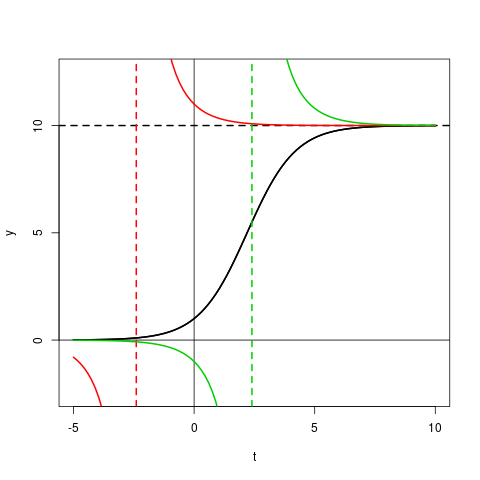
\includegraphics[width=.5\textwidth, trim=0 10 20 30, clip=]{Verhulst-solutions}
    \end{tabular}
  \end{tabular}
  $$
  On distingue donc deux comportements en temps long différents partant de $y(0) = y_0$ : 
  \begin{itemize}
    \item si $y(0) = y_0 > K$ (soit $t^* < 0$), on a toujours
    $$
    \lim_{t \to \infty} y(t) = K,
    $$
    et $y^* = K$ est un équilibre stable ;
    \item si $y(0) = y_0 < 0$ (soit $t^* > 0$), la limite précédente reste vraie, mais, puisque
    $$
    \lim_{t \uparrow t^*} y(t) 
    = \lim_{t \uparrow -\log(-a_0) / r}  \frac{K a_0 e^{rt}}{1 +  a_0 e^{rt}}
    = -\infty,
    $$
    $y(t)$ atteint $- \infty$ en un temps fini $t^*$. $y^* = 0$ est donc un équilibre instable ($y^* = K$ est un équilibre stable, mais il ne sera jamais atteint).
  \end{itemize}
\end{description}

\remark
Le modèle de Verhulst est un des rares modèles non-linéaires pour lesquels il existe une solution explicite. Il n'est cependant pas nécessaire de disposer d'une solution explicite pour étudier la stabilité d'un équilibre.

\begin{theorem}[Stabilité ($n = 1$)]
  Pour $n=1$, un point d'équilibre $y^*$ est stable si $F'(y^*) < 0$ et instable si $F'(y^*) > 0$.
\end{theorem}

\proof Non démontré. \eproof

\remark
On obtient une intuition de ce résultat en étudiant la fonction $h(t) = y(t) - y^*$ au voisinage de $y(t) = y^*$. On a
$$
\dot h(t) = \dot y(t) = F(y(t)) = F(y^* + h(t)) = \underset{=0}{\underbrace{F(y^*)}} + F'(y^*) h(t) + o(\|h(t)\|),
$$
$h(t)$ se comporte donc localement comme la solution de 
$$
\dot h(t) = F'(y^*) h(t)
$$
soit $e ^{F'(y^*) t}$ qui tend vers 0 si $F'(y^*) < 0$ et vers l'infini si $F'(y^*) > 0$.

\exemple{
  Dans le cas du modèle de Verhulst, on a $F(y) = y(r - cy)$, soit
  $$
  F'(y) = r - 2cy
  $$
  qui est bien positive pour $y = 0$ (équilibre instable) et négative pour $y = K = r/c$ (équilibre stable).
}

%-------------------------------------------------------------------------------
\paragraph*{Notion de bifurcation.}
De nombreux systèmes dynamiques sont exprimés en fonction de paramètres dont dépendent les points d'équilibre et leur nature. Des valeurs proches des paramètres donnent des points d'équilibres proches et de même nature. La théorie des bifurcations s'intéresse aux régions de l'espace des paramètres au sein desquelles les points d'équilibres restent de même nature : plus précisément elle s'intéresse aux frontières entre ces régions.

%-------------------------------------------------------------------------------
\exemple{
  On étudie les points d'équilibre du système 
  $$
  \dot y = F(y) = \mu y - y^3
  $$
  et on souhaite déterminer leur nature. \\
  On a 
  $$
  F(x) = x(\mu - x^2) = 0 
  \qquad \Leftrightarrow \qquad
  x \in \left\{\begin{array}{ll} 
      \{-\sqrt{\mu}, 0, \sqrt{\mu}\} & \text{si } \mu > 0 \\
      \{0\} & \text{si } \mu \leq 0
    \end{array}\right.
  $$ 
  De plus, 
  $$
  F'(x) = \mu - 3 x^2
  $$
  donc
  \begin{itemize}
    \item si $\mu < 0$, $0$ est le seul équilibre et il est stable, , 
    \item si $\mu > 0$, $0$ est instable mais $-\sqrt{\mu}$ et $\sqrt{\mu}$ sont stables. 
  \end{itemize}
  On peut ainsi tracer le {\em diagramme de bifurcation}.
  $$
%  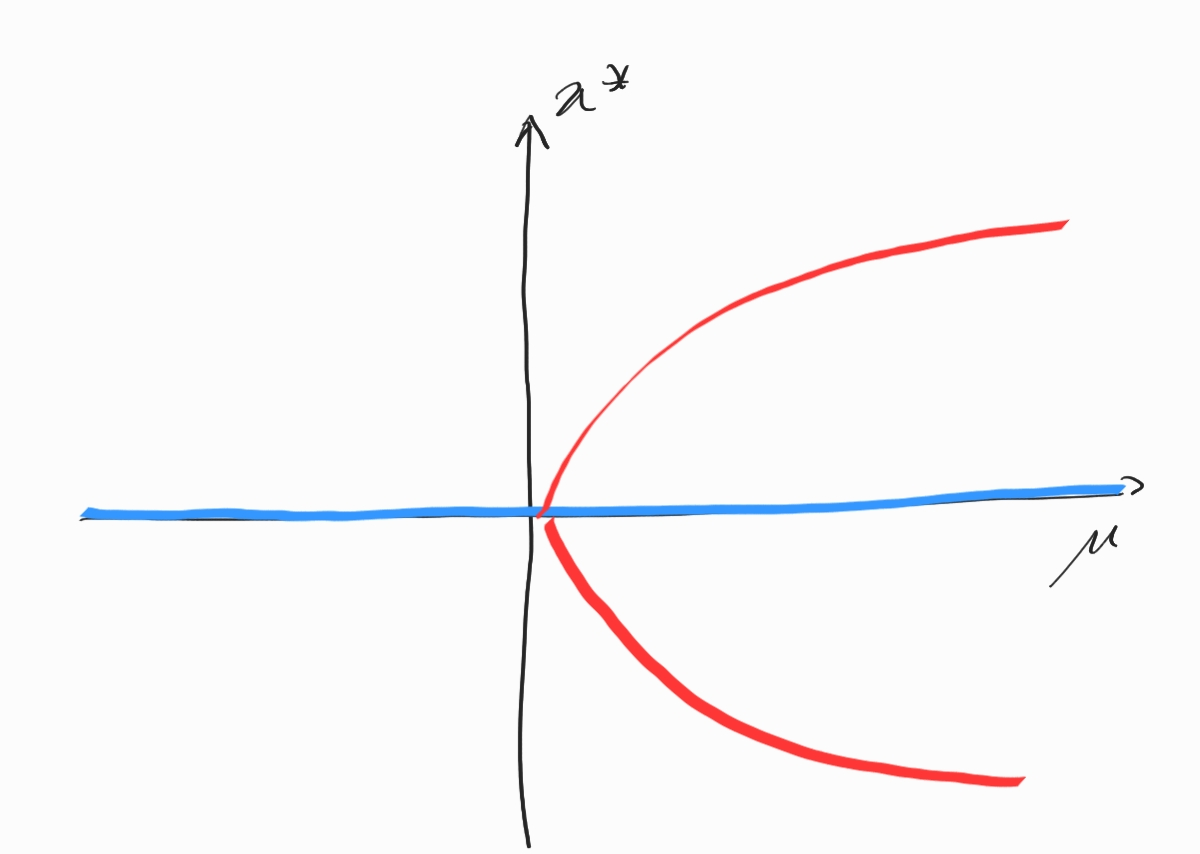
\includegraphics[width=.5\textwidth, trim=0 0 0 15, clip=]{StabiliteSystemeDynamique-Exemple1}
  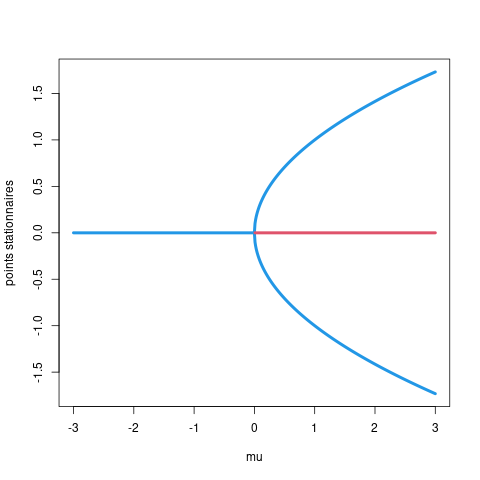
\includegraphics[width=.5\textwidth, trim=0 0 0 15, clip=]{StabiliteSystemeDynamique-Bifurcation}
  $$
}

% %-------------------------------------------------------------------------------
% \textcolor{gray}{
%   \exemple{
%     On souhaite déterminer les points d'équilibre (et leur nature) du système
%     $$
%     \dot y = F(y) = \mu y + 2 y^3 - y^5.
%     $$
%     On a 
%     $$
%     F(y) = y(\mu + y^2 - y^4)
%     $$
%     qui s'annule pour $y = 0$ et pour les solutions de $(\mu + 2 y^2 - y^4)$. En posant, $z = y^2$, $\mu + 2 z - z^2 = 0$ admet des solutions si $\Delta =  4(1 + \mu) \geq 0$, soit $\mu \geq -1$. Ces solutions sont alors $z^* = -1 \pm \sqrt{1+\mu}$. La seule solution possiblement positive est $z^* = -1 + \sqrt{1+\mu}$ et elle l'est ssi $\mu > 1$. \\
%     Le système admet donc un unique point fixe $y^*=0$ si $\mu < 1$ et un second point fixe $y^* = -1+\sqrt{1+\mu}$ si $\mu > 1$. \\
%     On a de plus
%     $$
%     F'(x) = \mu + 3 y^2 - 5y^4
%     $$
%     dont le signe est celui de $\mu$ pour $x=0$ et \todo{nature de $y^* = -1+\sqrt{1+\mu}$ si $\mu > 1$.}
%   }}

% %-------------------------------------------------------------------------------
% \exemple{[Exercice 2, TD2, L2 Bio SU]
%   On considère le système
%   $$
%   \dot y = - y^3 + 7 y^2 - 14 y + 8.
%   $$
%   Ses points stationnaires sont les racines du polynôme $P(y) = - y^3 + 7 y^2 - 14 y + 8$, donc $y_1 = 1$ fait partie, donc
%   $$
%   P(y) = (y-1) (-y^2 + 6y + 8),
%   $$
%   et les deux racines de $-y^2 + 6y + 8$ sont $2$ et $4$. Les points stationnaires du système sont donc 
%   $$
%   y_1 = 1, \qquad y_2 = 2, \qquad y_3 = 4.
%   $$
%   Leur stabilité est donné par la dérivée de $P$:
%   $$
%   P'(y) = -3y^2 + 14 y - 14,
%   $$
%   soit
%   $$
%   P'(y_1) = -3, \qquad P'(y_2) = 2, \qquad P'(y_3) = -6.
%   $$
%   $y_1$ et $y_3$ sont donc des équilibres stables, et $y_2$ un équilibre instable.
%   $$
%   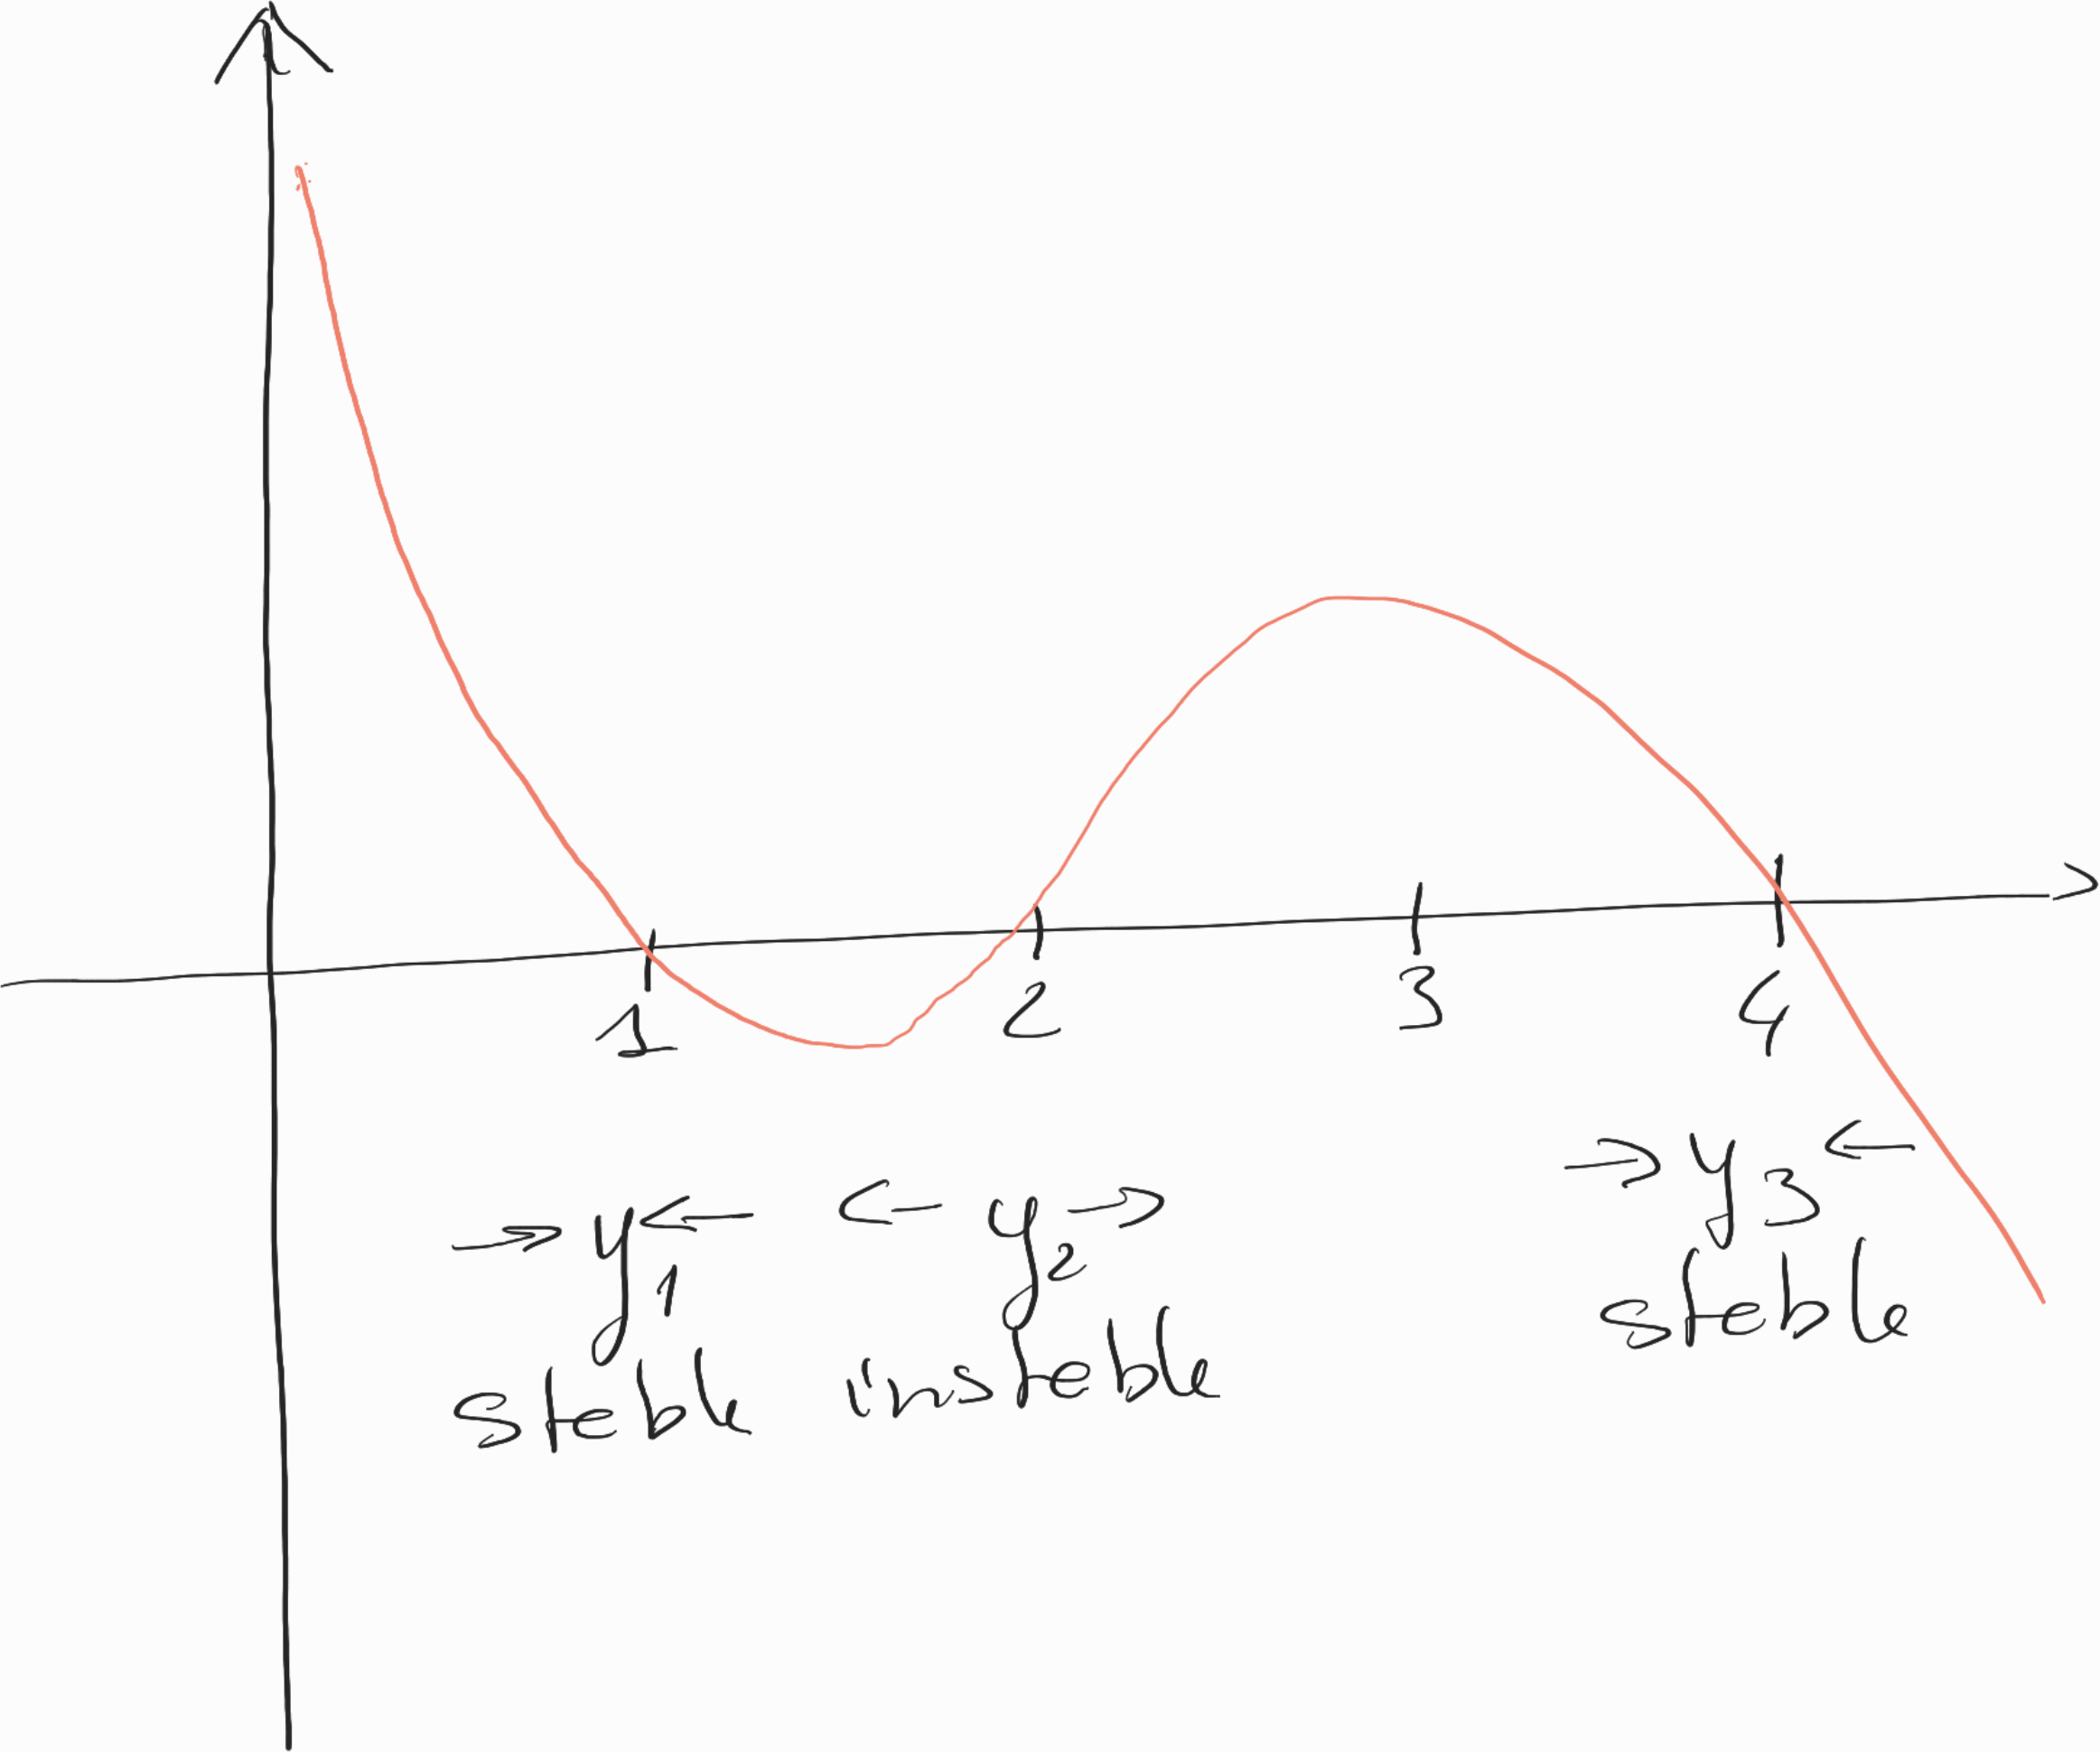
\includegraphics[width=.5\textwidth]{TD-SUbioL3-TD2Exo2}
%   $$
% }

\newpage %-------------------------------------------------------------------------------
%-------------------------------------------------------------------------------
\section{ODE en dimension $n$} \label{sec:EquaDiff-nonLineaire}
%-------------------------------------------------------------------------------

%-------------------------------------------------------------------------------
\subsection{ODE linéaire en dimension $n$.}
%-------------------------------------------------------------------------------

\begin{definition}
  Une ODE $\dot y = F(y)$ est dite linéaire si l'application $F : \Rbb \mapsto \Rbb$ est linéaire : 
  $$
  \dot y (t) = A y(t).
  $$
\end{definition}

\remark
Les points d'équilibre $y^*$ sont les élément du noyau $\ker(A)$, i.e. les vecteurs propres associés à la valeur propre 0. En conséquence, {\sl si $\lambda = 0$ n'est pas valeur propre de $A$}, il n'existe pas d'autre point stationnaire que $y^* = 0_n$.

%-------------------------------------------------------------------------------
\paragraph*{Cas diagonalisable.}

\begin{proposition}[ODE linéaire diagonalisable] \label{prop:odeLineaireDiagonalisable}
  Si la matrice $A$ est diagonalisable : 
  $$
  A = P D P^{-1}
  \qquad \text{avec}  \quad 
  D = \diag(\lambda_1, \dots \lambda_n),
  $$
  la solution du problème
  $$
  \{y(0) = y_0, \; \dot y = A y\}
  $$
  est
  $$
  y(t) = P E(t) P^{-1} y_0  
  $$
  avec
  $$
  E(t) = \diag\left(e^{\lambda_1 t} \dots e^{\lambda_n t} \right).
  $$
\end{proposition}

% {Démonstration de la proposition \ref{prop:odeLineaireDiagonalisable}.}
\proof
En posant $z(t) = P^{-1} y(t)$ et puisque la dérivation est linéaire, il vient 
$$
\dot z (t) = P^{-1} \dot y(t) = P^{-1} A y(t) = P^{-1} P D P^{-1} y(t) = D z(t).
$$
On obtient ainsi que les fonctions $z_i(t)$ sont respectivement solutions de $\dot z_i = \lambda_i z_i$, soit 
$$
z_i(t) = z_{0i} e^{\lambda_i t}
$$
avec $z_0 = z(0) = P^{-1} y(0) = P^{-1} y_0$. La solution s'obtient en revenant à $y(t) = P z(t)$.
\eproof

%-------------------------------------------------------------------------------
\begin{definition}[Exponentielle de matrice]
  L'exponentielle matricielle est la fonction
  $$
  \begin{array}{rccc}
    \exp: & \Mcal_n(\Rbb) & \mapsto & \Mcal_n(\Rbb) \\
      & B & \to & \exp(B),
  \end{array}
  \qquad \text{où} \quad
  \exp(B) = \sum_{k \geq 0} \frac{B^k}{k !}
  $$
\end{definition}

\exemple{[Exponentielle d'un matrice diagonale]
  Soit $D = \diag[d_1, \dots d_n]$, on a
  \begin{align*}
    \exp(D) 
    & = \sum_{k \geq 0} \frac{D^k}{k !}
    = \sum_{k \geq 0} \frac1{k !} \diag[d_1^k, \dots d_n^k]
    = \diag[\exp(d_1), \dots \exp(d_n)].
  \end{align*}
}

%-------------------------------------------------------------------------------
\remarks
\begin{enumerate}
  \item La proposition \ref{prop:odeLineaireDiagonalisable} dit que, au prix du changement de base $z = P^{-1} y$, le système $\dot y = A y$ est équivalent à $n$ équations différentielles linéaires unidimensionnelles ($\dot z = D z$).
  \item La condition initiale $y_0$ se décompose sous la forme
  $$
  y_0 = P z_0 = \sum_i z_{i0} v_i
  $$
  où les $v_i$ sont les vecteur propres de $A$, i.e. les vecteurs colonnes de $P$.
  \item En définissant l'exponentielle matricielle
  $$
  \exp(B) = \sum_{k \geq 0} \frac1{k!} B^k
  \qquad \Rightarrow \qquad
  \exp(P B P^{-1}) = P \exp(B) P^{-1}
  $$
  on obtient ainsi que
  $$
  E(t) = \exp(t D) 
  \qquad \text{et} \qquad 
  P E(t) P^{-1} = P \exp(t D) P^{-1} = \exp(t P D P^{-1}) = \exp(t A).
  $$
  On retrouve ainsi que la solution du problème
  $$
  \{y(0) = y_0, \; \dot y = A y\}
  $$
  s'écrit
  $$
  y(t) = \underset{\in \Mcal_n}{\underbrace{\exp(t A)}} \; y_0.
  $$
  \item On peut étudier le comportement en temps long du système en considérant
  \begin{align*}
    \lim_{t \to \infty} y(t)
    & = \lim_{t \to \infty} \exp(t A) y_0 
    = P \left(\lim_{t \to \infty} \exp(t D)\right) \underset{z_0}{\underbrace{P^{-1} y_0}}
    = \sum_{i=1}^n \left(z_{0i} \lim_{t \to \infty} e^{\lambda_i t}\right) v_i.
  \end{align*}
  Comme
  $$
  \lim_{t \to \infty} e^{\lambda_i t} = 
  \left\{\begin{array}{rr}
          0 & \text{si } \lambda_i < 0 \\
          1 & \text{si } \lambda_i = 0 \\
          +\infty & \text{si } \lambda_i > 0
         \end{array}\right.
  $$
  on peut donc distinguer deux cas : 
  \begin{itemize}
  \item soit il existe $\lambda_i > 0$ telle que $z_{0i} \neq 0$, et on a alors
  $$
  \lim_{t \to \infty} \|y(t)\| = + \infty
  $$
  (le système explose dans la direction $v_i$), 
  \item soit le système tend vers une combinaison linéaire d'éléments du noyau de $A$ :
  $$
  \sum_{i : \lambda_i = 0} z_{0i} v_i \in \ker(A)
  $$
  qui dépend de la condition initiale $y_0 = P z_0$.
  \end{itemize}
  En conclusion, s'il existe au moins un $\lambda_i \geq 0$, un perturbation autour d'un point d'équilibre $y^* \in \ker(A)$ éloignera le système de $y^*$ dans la direction $v_i$. A l'opposé, si toutes les $\lambda_i$ sont strictement négatives, quelque soit $y_0$, $\lim_{t \to \infty} y(t) = 0$ qui est donc le seul équilibre stable.
\end{enumerate}

%-------------------------------------------------------------------------------
\paragraph*{Cas non diagonalisable.}

\begin{theorem}
  Soit $A$ non diagonalisable et $\lambda_1, \dots \lambda_n$ les racines (possiblement complexes, non nécessairement distinctes) de son polynôme caractéristique, quelque soit $y_0$, il existe $n^2$ polynômes (à coefficients complexes) $q_{ij}(t)$ tels quel la solution du problème
  $$
  \{y(0) = y_0, \; \dot y = A y\}
  $$
  soit
  $$
  y_i(t) = \sum_{j=1}^n q_{ij}(t) e^{\lambda_j t}.
  $$
  En conséquence, 0 est le seul équilibre stable possible et il l'est à condition que
  $$
  \forall 1 \leq i \leq n: \quad \Re(\lambda_i) < 0
  $$
  en notant $\Re(u)$ la partie réelle du nombre complexe $u$.
\end{theorem}

\proof Non démontré. \eproof

% \progres{
%   Rappel cours 5 :
%   \begin{itemize}
%     \item Equation différentielle ordinaire en dimension 1
%     \item Stabilité des points stationnaires
%     \item Equation différentielle ordinaire en dimension $n$ : $A$ diagonale, diagonalisable
%   \end{itemize}
%   Programme cours 6 :
%   \begin{itemize}
%     \item Equation différentielle ordinaire non-linéaire en dimension $n$, linéarisation
%     \item Equation différentielle ordinaire non-linéaire en dimension $2$
%   \end{itemize}
% }

%-------------------------------------------------------------------------------
\subsection{Linéarisation} 
%-------------------------------------------------------------------------------

On souhaite maintenant étudier la nature des équilibres d'un système non linéaire. En dimension 1, cet analyse s'est fondée sur la dérivée de la fonction $F$. Le théorème suivant généralise cette représentation fondée sur l'approximation au premier ordre aux abords d'un équilibre $y^*$ en posant $y(t) = y^* + h(t)$: 
$$
\dot h(t) = \dot y (t) = F(y(t)) = F(y^* + h(t)) 
\simeq \underset{=0}{\underbrace{F(y^*)}} + (D_{y^*} F)(h(t)) = J_{y^*} h(t).
$$

%-------------------------------------------------------------------------------
\begin{theorem}[Hartman-Grobman]
  Le point d'équilibre $y^*$ de l'ODE $\dot y = F(y)$ a la même nature que l'origine $0$ pour le système linéaire 
  $$
  \dot y = (J_{y^*}F) \; . \; y
  $$
  à condition que toutes les valeurs propres de $J_{y^*}$ aient une partie réelle non nulle. \\
  En particulier, $y^*$ est stable si $\forall i: \Re(\lambda_i) < 0$.
\end{theorem}

\proof Non démontré. \eproof

%-------------------------------------------------------------------------------
\paragraph*{Démarche.}
On peut ainsi définir une démarche systématique pour étudier les équilibres d'un système $\dot y = F(y)$ :
\begin{enumerate}
  \item Trouver les points équilibres en déterminant d'abord les {\em isoclines}
  $$
  \Ical_k = \{y : F_k(y) = 0\}
  $$
  puis leur intersection $\bigcap_k \Ical_k$ pour déterminer les racines $y^*$ de  $F(x) = 0$ ;
  \item Calculer la matrice jacobienne $J_{y^*} F$ pour chaque équilibre $y^*$ ;
  \item Déterminer les racines du polynôme caractéristique $P_{J_{y^*}}(\lambda)$ et en déduire la nature de $y^*$ si toutes les racines ont une partie réelle non nulle.
\end{enumerate}

% \vspace{.1\textheight}
% \progres{
%   Début Cours 8. Rappels :
%   \begin{enumerate}[\itemdot]
%     \item Système dynamique défini ppour $y(t) \Rbb^n$:
%     $$
%     \{y(t_0 = y_0, \; \dot y = F(y)\}
%     $$
%     \item Point d'équilibre $y^*$ : $F(x) = 0$
%     \item ($n = 1$) Nature de $y^*$: stable si $F'(y^*) < 0$, instable si $F'(y^*) > 0$.
%     \item ($n \geq 1$) Cas linéaire diagonalisable : caractérisation en fonction du signe des valeurs propres \\
%     $\Rightarrow$ 0 seul équilibre stable possible (à condition que tous les $\lambda_i < 0$) \\
%     $\Rightarrow$ idem cas non-diagonalisable
%     \item ($n \geq 1$) Cas non linéaire : nature d'une équilibre $y^*$ = même nature que l'origine pour le système linéaire avec $A = J_{y^*} F$.
%   \end{enumerate}
% }

\newpage %-------------------------------------------------------------------------------
%-------------------------------------------------------------------------------
\section{ODE en dimension 2} \label{sec:EquaDiff-nonLineaire2D}
%-------------------------------------------------------------------------------

On s'intéresse ici au cas d'une système d'ODE $\dot y = F(y)$ avec $F : \Rbb^2 \mapsto \Rbb^2$. 

%-------------------------------------------------------------------------------
\subsection{Classification des équilibres} 
%-------------------------------------------------------------------------------

La classification des équilibres repose sur l'étude des valeurs propres $\lambda_1$ et $\lambda_2$ de la matrice jacobienne $J_{y^*}$ en tout point d'équilibre $y^*$ solution de $F(y^*) = 0$. On peut ainsi définir la classification suivante :
$$
\begin{tabular}{ll}
  $(\lambda_1, \lambda_2) \in \Rbb, (\lambda_1, \lambda_2) < 0 :$ & point stable ou 'puit' ; \\
  $(\lambda_1, \lambda_2) \in \Rbb, (\lambda_1, \lambda_2) > 0 :$ & point instable ou 'source' ; \\
  $(\lambda_1, \lambda_2) \in \Rbb, \lambda_1 > 0 , \lambda_2 < 0 :$ & point selle ; \\
  $(\lambda_1, \lambda_2) \in \Cbb, \Re(\lambda_1, \lambda_2) < 0 :$ & point de concentration ou 'puit en spirale' ; \\
  $(\lambda_1, \lambda_2) \in \Cbb, \Re(\lambda_1, \lambda_2) > 0 :$ & point de repulsion ou 'source en spirale'. \\
  $(\lambda_1, \lambda_2) \in \Cbb \setminus \Rbb:$ & voir ci-dessous.
\end{tabular}
$$

\begin{figure}[ht]
  \begin{center}
    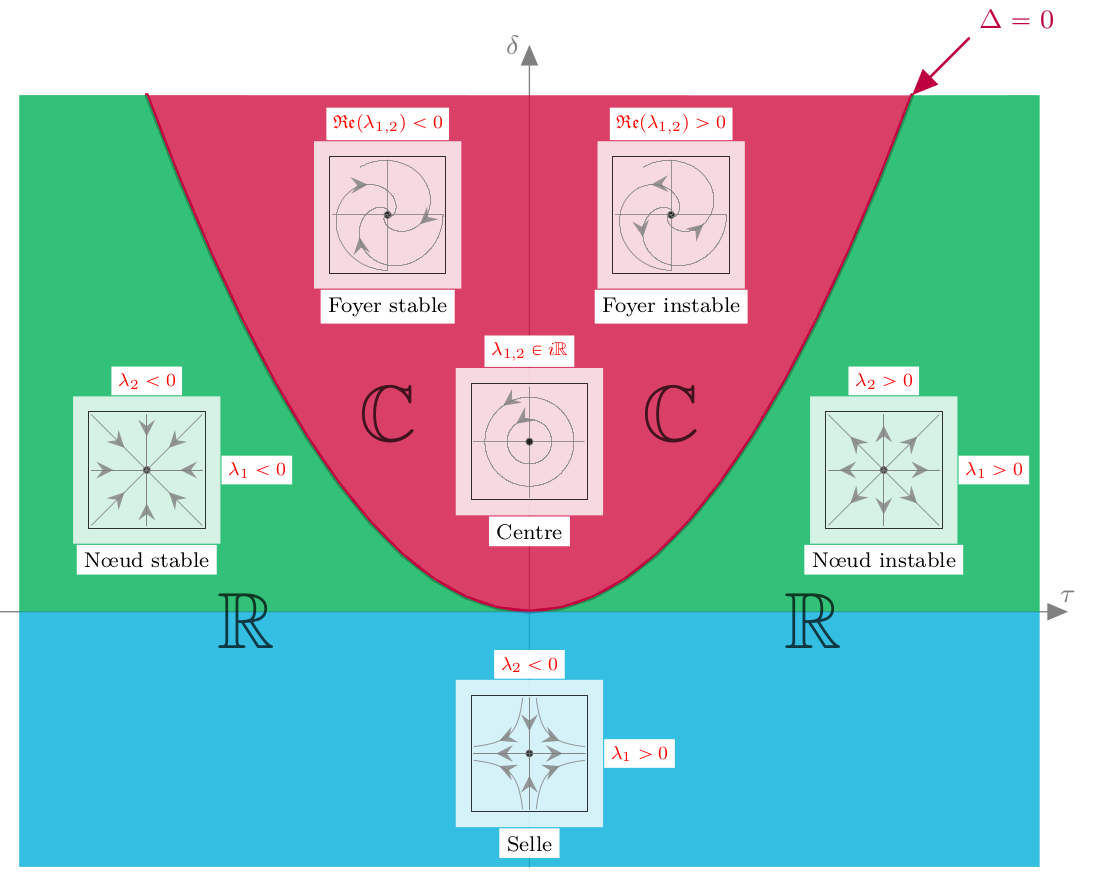
\includegraphics{L3-SU-MathBio-StabiliteEquilibresD2}
  \end{center}
  \caption{Stabilité des équilibres en dimension 2. $\tau = \tr(A)$, $\delta=|A|$, $\Delta = \tau^2 - 4 \delta$ (discriminant de $P_A(\lambda)$.}
\end{figure}

Les théorèmes vus jusqu'à présent ne permettent pas d'étudier le dernier cas, qui correspond à des trajectoires limites cycliques.

%-------------------------------------------------------------------------------
\subsection{Existence d'orbites périodiques} 
%-------------------------------------------------------------------------------

\begin{definition}[Orbite]
  Pour toute solution $(f, I)$ d'une ODE, on appelle \emph{orbite} l'ensemble $\{f(t), t \in I\}$. S'il existe $t_0$ tel que $[t_0, \infty) \subset I$, l'ensemble $\{f(t), t \geq t_0\}$ est appelé \emph{semi-orbite positive}.
\end{definition}

%-------------------------------------------------------------------------------
\begin{theorem}[Poincarré-Bendixson]
  Soit $D$ un fermé borné de $\Rbb^2$ ne contenant pas de point d'équilibre d'une ODE $\dot y = F(y)$. S'il existe une semi-orbite positive $O$ entièrement comprise dans $D$ alors l'ensemble $C$ des points limite de $O$ est une orbite périodique. Si $O$ n'est pas l'ensemble $C$, $C$ et appelé cycle limite.
\end{theorem}

\remark
Le théorème dit que si une trajectoire solution de l'ODE est piégée dans une région $D$ bornée de $\Rbb^2$, elle doit se rapprocher de plus en plus d'une courbe $C$ fermée. Il n'est souvent pas difficile d'identifier une telle région $D$, mais déterminer le cycle limite $C$ est souvent plus difficile.

%-------------------------------------------------------------------------------
\paragraph*{Détermination d'un cycle.} 

\begin{definition}[Hamiltionien]
  Un hamiltionien (ou une fonction hamiltonienne) d'une ODE est une fonction $H : \Rbb^n \mapsto \Rbb$ qui reste constante le long des trajectoires solution de l'ODE.
\end{definition}

\remark
Cette définition revient à dire que les solutions $y(t)$ suivent des lignes de niveau de la fonction hamiltonienne.

\bigskip
\begin{proposition}[Hamiltionien] \label{prop:hamiltonien}
  Si $H$ est un hamiltonien de l'EDO $\{\dot y = F(y), y(0) = y_0\}$, où $F$ est une application de $\Rbb^n$ dans $\Rbb^n$, il vérifie :
  $$
  \sum_{i=1}^n F_i(y) \left.\frac{\partial H}{\partial y_i}\right|_{y(t)} = 0.
  $$
\end{proposition}

% {Démonstration de la proposition \ref{prop:hamiltonien}.}
\proof
  La définition du hamiltonien impose que 
  $$
  \frac{\partial}{\partial t} H(y(t)) \equiv 0.
  $$
  Pour déterminer la dérivée de $H(y(t))$ par rapport au temps, on utilise la proposition \ref{prop:compositionDifferentielles} avec $f = H$ et $g = y$, soit
%   $$
%   \begin{array}{rrcl}
%     f : & \Rbb^n & \mapsto & \Rbb \\
%     & y & \to & f(y) = H(y)
%   \end{array},
%   \qquad
%   \begin{array}{rrcl}
%     g : & \Rbb & \mapsto & \Rbb^n \\
%     & t & \to & g(y) = y(t)
%   \end{array},
%   $$
%   soit
  $$
  \frac{\partial}{\partial t} H(y(t)) 
  = J_{y(t)}H \cdot J_ty
  $$
  où
  $$
  J_{y(t)}H = \left[ \begin{array}{ccc}
    \displaystyle{\left.\frac{\partial H}{\partial y_1}\right|_{y(t)}} & 
    \dots & 
    \displaystyle{\left.\frac{\partial H}{\partial y_n}\right|_{y(t)}} 
  \end{array}\right] 
  \qquad \text{et} \qquad 
  J_ty = \left[\begin{array}{c} 
    \dot y_1(t) = F_1(y(t)) \\
    \vdots \\
    \dot y_1(t) = F_n(y(t))
  \end{array}\right] 
  $$
\eproof

%-------------------------------------------------------------------------------
\paragraph*{Cas $n = 2$.} 
On considère une ODE avec $F : \Rbb^2 \mapsto \Rbb^2$ : 
$$
\left\{\begin{array}{rcl} \dot x & = & F_1(x, y) \\ \dot y & = & F_2(x, y) \end{array}\right.
$$
Soit $(x(t), y(t))$ une solution maximale sur $I$ pour la condition initiales $(x(t_0), y(t_0)) = (x_0, y_0)$. Un hamitonien est une fonction $H : \Rbb^2 \mapsto \Rbb^2$ qui vérifie
$$
\forall t \in I: \quad H(x(t), y(t)) = H(x_0, y_0).
$$
Les orbites sont alors les lignes de niveau du hamiltonien : 
$$
\Ccal_z = \{x, y: H(x, y, ) = z\}.
$$

La difficulté réside alors dans la détermination d'une fonction $H$ qui vérifie la proposition \ref{prop:hamiltonien} en dimension 2 : 
\begin{align} \label{eq:derivHnulleD2}
  \dot x(t) \frac{\partial H}{\partial x} (x(t), y(t)) +
  \dot y(t) \frac{\partial H}{\partial y} (x(t), y(t)) & = 0 \nonumber \\
  \Leftrightarrow \qquad 
  F_1(x, y) \frac{\partial H}{\partial x} (x, y) +
  F_2(x, y) \frac{\partial H}{\partial y} (x, y) & = 0
\end{align}

%-------------------------------------------------------------------------------
\paragraph*{Cas ``séparable''.} 
On peut chercher une fonction $H$ séparable, c'est-à-dire de la forme
$$
H(x, y) = h_1(x) + h_2(y).
$$
On a alors
$$
\frac{\partial H}{\partial x} = h_1'(x), \qquad
\frac{\partial H}{\partial y} = h_2'(x)
$$
et la condition \eqref{eq:derivHnulleD2} devient
$$
F_1(x, y) h_1'(x) = -F_2(x, y) h_2'(y)
\qquad \Leftrightarrow \qquad
\frac{F_1(x, y)}{F_2(x, y)} = -\frac{h_2'(y)}{h_1'(x)}.
$$
On peut donc déterminer un hamiltonien de la forme $H(x, y) = h_1(x) + h_2(y)$ si on peut trouver $f$ et $g$ telles que
$$
\frac{F_1(x, y)}{F_2(x, y)} = \frac{g(y)}{f(x)}.
$$
Il reste alors à déterminer des fonctions $h_1$ et $h_2$ satisfaisant
$$
h'_1(x) = k f(x), \qquad
h'_2(y) = - k g(y).
$$
On utilisera cette méthode pour caractériser les cycles du modèle de Lotka-Volterra.

\newpage %-------------------------------------------------------------------------------
%-------------------------------------------------------------------------------
\section{Deux modèles classiques}
%-------------------------------------------------------------------------------

% Exercices sur la dynamique proie-prédateur, équations de Lotka–Volterra. Cycles et cycles-limites. Théorème de Poincaré–Bendixson. Bifurcations (selle-nœud, transcritique, en fourche, de Hopf). Le modèle SIR (sain et susceptible – infecté – sain et immunisé) de Kermack–McKendrick.

%-------------------------------------------------------------------------------
\subsection{Modèle de Lotka-Volterra}
%-------------------------------------------------------------------------------

On rappelle le modèle pour $y(t) = [N(t) \; P(t)]^\top$ où $N(t)$ est le nombre de proies au temps $t$ et $P(t)$ le nombre prédateurs au temps $t$:
$$
\left\{ \begin{array}{rclcl} 
  \dot N & = & r N - c N P & = & \displaystyle{r N \left( 1 - \frac{cP}r \right)} \\
  \dot P & = & b N P  - m P & = & \displaystyle{m P \left( \frac{bN}m - 1 \right)} 
\end{array} \right.
$$
et où les paramètres $r$, $c$, $b$, $m$ sont tous positifs ou nuls.

%-------------------------------------------------------------------------------
\paragraph*{Cas particuliers.}
\begin{description}
  \item[$P(t) = 0 $ (absence de prédateur) :] le système devient alors $\{\dot N = r N, \dot P \equiv 0\}$ dont la solution est $N(t) = N_0 e^{rt}$ : la population de proies explose comme dans un modèle de Mathus.
  \item[$N(t) = 0 $ (absence de proie) :] le système devient alors $\{\dot N \equiv 0, \dot P = - m P\}$ dont la solution est $P(t) = P_0 e^{-mt}$ : la population de prédateurs s'éteint à vitesse exponentielle.
\end{description}

%-------------------------------------------------------------------------------
\paragraph*{Changement de variable.}
Pour mener l'analyse mathématique de ce modèle, il est confortable de ``reparamétriser'' le problème, c'est-à-dire de poser
$$
x(t) = \frac{b}m N(t)
\qquad \text{et} \qquad
y(t) = \frac{c}r P(t).
$$
Le modèle devient alors
$$
\left\{\begin{array}{rcrcl} 
  \dot x & = & r x (1-y) & =: & F_1(x, y) \\
  \dot y & = & -m y (1-x) & =: & F_2(x, y)
\end{array}\right.
$$
où $x$ est proportionnel aux nombre de proies et $y$ au nombre de prédateurs.

%-------------------------------------------------------------------------------
\paragraph*{Points d'équilibres.}
On détermine d'abord les isoclines en annulant chacune des fonctions $F_1$ et $F_2$ :
\begin{align*}
  F_1(x, y) & = 0 \quad \Leftrightarrow \quad x = 0 \text{ ou } y = 1 &
  \Rightarrow \qquad \Ical_1 & = \{x = 0\} \cup \{y = 1\}, \\
  F_2(x, y) & = 0 \quad \Leftrightarrow \quad y = 0 \text{ ou } x = 1 &
  \Rightarrow \qquad \Ical_2 & = \{x = 1\} \cup \{y = 0\}.
\end{align*}
Les équilibres sont donnés par l'intersection 
$$
\Ical_1 \cap \Ical_2 = \{(0, 0), (1, 1)\}
$$

%-------------------------------------------------------------------------------
\paragraph*{Nature des équilibres.}
Pour déterminer la nature des équilibres, on étudie la matrice jacobienne
$$
J_{(x, y)}F = 
  \left[\begin{array}{ccc} 
    r (1-y) & & -r x \\
    m y & & -m (1-x)
  \end{array}\right].
$$

%-------------------------------------------------------------------------------
\paragraph*{\'Etude de $(x^* = 0, y^* = 0)$.}
On a 
$$
J_{(0, 0)}F = 
  \left[\begin{array}{rcr} 
    r  & & 0 \\
    0 & & -m 
  \end{array}\right]
$$
dont les deux valeurs propres de $J_{(0, 0)}F$ sont $r$ et $-m$, qui sont de signes opposés. Il s'agit donc d'un point selle. En effet $(0, 0)$ est stable dans une direction : 
\begin{itemize}
  \item en l'absence de proie, l'apparition de quelques prédateurs ramène le système vers $(0, 0)$, 
  \item en l'absence de prédateur, l'apparition de quelques proies mène à une explosion de leur population.
\end{itemize}
  
%-------------------------------------------------------------------------------
\paragraph*{\'Etude de $(x^* = 1, y^* = 1)$.}
On a 
$$
J_{(1, 1)}F = 
  \left[\begin{array}{rcr} 
    0 & & -r  \\
    m  & & 0
  \end{array}\right]
$$
dont le polynôme caractéristique est $P(\lambda) = \lambda^2 + rm$ qui s'annule pour
$$
\lambda = \pm i \sqrt{rm}.
$$
Les deux valeurs propres sont des imaginaires pures : on peut chercher un hamiltonien du système pour étudier ce point d'équilibre.

\bigskip
On remarque que 
$$
\frac{F_1(x, y)}{F_2(x, y)} = -\frac{rx(1-y)}{my(1-x)} = \frac{g(y)}{f(x)}
$$
où
\begin{align*}
f(x) = -m \frac{(1-x)}{x} = m \left(1 - \frac1x\right), \qquad
g(y) = r \frac{(1-y)}{y} = r \left(\frac1y - 1\right).
\end{align*}
En choisissant 
\begin{align*}
  h_1(x) = m(x-\log(x)), \qquad h_2(x) = r(y-\log(y)),
\end{align*}
on vérifie bien que $h'_1(x) = -f(x)$ et $h'_2(x) = g(y)$ et que 
$$
H(x, y) = m(x-\log(x)) + r(y-\log(y))
$$
est bien un hamiltonien : 
\begin{align*}
\dot H 
& = m\left(1 - \frac1x\right) \dot x + r \left(1 - \frac1y\right) \dot y \\
& = m\left(1 - \frac1x\right) r x (1 - y) + r \left(1 - \frac1y\right) (- m y (1 - x)) 
% & = m r (x - 1) ( 1 - y) - r  m (y - 1) (1 - x) 
= 0.
\end{align*}

\bigskip
Il reste à démontrer que les lignes de niveau $\Ccal_z$ de $H$ sont des courbes closes. Il suffit pour cela de démontrer que $H$ est convexe avec un minimum global (ou concave avec un maximum global). On a
$$
\nabla H = \left[\begin{array}{c} m(1 - 1/x) \\ r(1 - 1/y)\end{array}\right], 
$$
qui s'annule uniquement pour $(x^* = 1, y^*=1)$. On a de plus
$$
\nabla^2 H = \left[\begin{array}{ccc} m/x^2 & & 0 \\ 0 & & r/y^2 \end{array}\right] 
$$
qui est (strictement) définie positive.
$H$ admet donc un unique minimum en $(x^* = 1, y^*=1)$ et est partout strictement convexe : ses lignes de niveaux sont donc closes.

\bigskip
Partant d'un état ($x_0, y_0$), le système suit une trajectoire cyclique 
correspondant à la ligne de niveau $\Ccal_{z_0}$ où $z_0 = H(x_0, y_0)$.

\dessin{
$$
\begin{tabular}{ccc}
  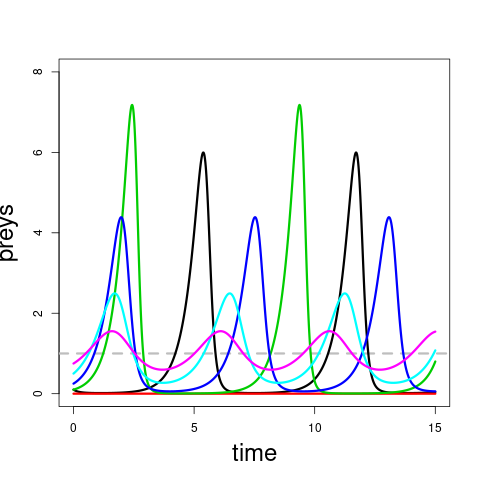
\includegraphics[width=.3\textwidth]{LotkaVolterra-preys} &
  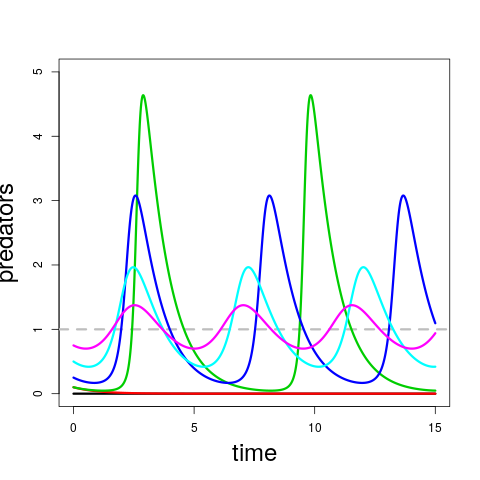
\includegraphics[width=.3\textwidth]{LotkaVolterra-predators} &
  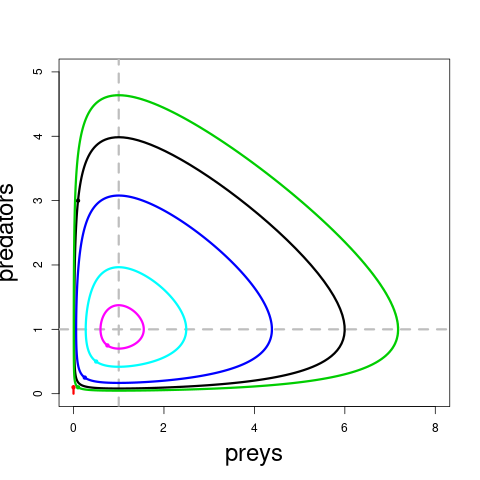
\includegraphics[width=.3\textwidth]{LotkaVolterra-preysPredators} \\
  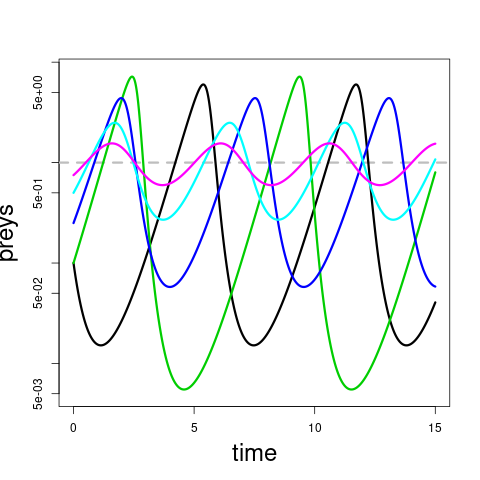
\includegraphics[width=.3\textwidth]{LotkaVolterra-preysLog} &
  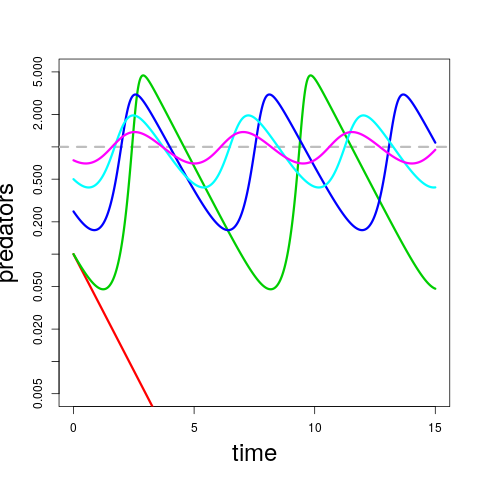
\includegraphics[width=.3\textwidth]{LotkaVolterra-predatorsLog} &
  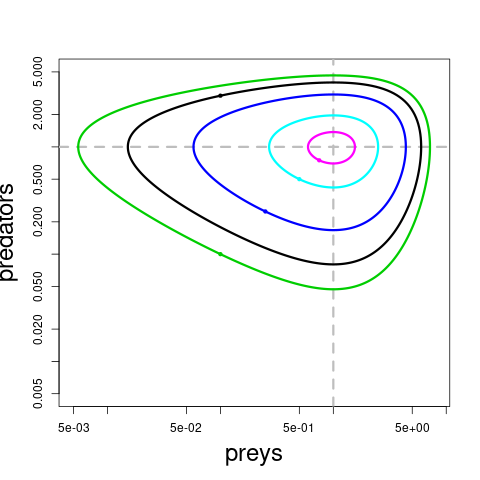
\includegraphics[width=.3\textwidth]{LotkaVolterra-preysPredatorsLog} \\
\end{tabular}
$$
}

%-------------------------------------------------------------------------------
\subsection{Modèle SIR = modèle de Kermack - McKendrick}
%-------------------------------------------------------------------------------

On rappelle le modèle pour $y(t) = [S(t) \; I(t) \; R(t)]^\top$ avec $S(t) =$ nombre de susceptibles au temps $t$, $I(t) =$ nombre d'infectés et $R(t) =$ nombre de 'remis' ({\em recovered}) :
$$
\left\{ \begin{array}{rclcl} 
\dot S & = & - r S I \\
\dot I & = & r S I - a I & = & \displaystyle{a \left(\frac{rS}a  - 1\right)} \\
\dot R & = & a I \\
\end{array} \right.
$$
$r$ contrôle le taux d'infection et $a$ le taux de rémission.

%-------------------------------------------------------------------------------
\paragraph*{Changement de variables.}
On remarque que $\dot S + \dot I + \dot R = \dot (S + I + R) = 0$, soit 
$$
S(t) + I(t) + R(t) = \cst.
$$
On peut donc se contenter d'étudier $\{S(t), I(t), t \geq 0\}$. On peut de plus poser 
$$
x(t) = \frac{rS}a, \qquad y(t) = I,
$$
soit
$$
\left\{\begin{array}{rclcl}
        \dot x & = & -r x y & =: & F_1(x, y) \\
        \dot y & = & a y (x - 1) & =: & F_2(x, y)
       \end{array}\right.
$$

\remarks
\begin{enumerate}
  \item $\dot x = - rxy$ est toujours négative : la population de susceptibles décroît systématiquement ; 
  \item la croissance du nombre de susceptible $y = I$ dépend de la position de $x$ par rapport à 1 :
  $$
  \left\{\begin{array}{lllll}
                \dot y < 0 & & (y \downarrow) & \text{si } x > 1, \\
                \dot y = 0 & & (y = \cst) & & \text{si } x = 1, \\
                \dot y > 0 & & (y \uparrow) & & \text{si } x < 1,
                \end{array}\right..
  $$
\end{enumerate}

\dessin{Dessiner le champ de vecteurs $(\dot x, \dot y)$}

%-------------------------------------------------------------------------------
\paragraph*{Points d'équilibres.}
\begin{align*}
  F_1(x, y) & = 0 \quad \Leftrightarrow \quad x = 0 \text{ ou } y = 0 &
  \Rightarrow \qquad \Ical_1 & = \{x = 0\} \cup \{y = 0\}, \\
  F_2(x, y) & = 0 \quad \Leftrightarrow \quad y = 0 \text{ ou } x = 1 &
  \Rightarrow \qquad \Ical_2 & = \{x = 1\} \cup \{y = 0\}.
\end{align*}
Les équilibres sont donnés par l'intersection 
$$
\Ical_1 \cap \Ical_2 = \{y = 0\}
$$

%-------------------------------------------------------------------------------
\paragraph*{Nature des équilibres.}
On calcule la jacobienne
$$
J_{(x, y)}F = 
  \left[\begin{array}{rcr} 
    - r y & & -r x \\
    - a y & & a (x - 1)
  \end{array}\right].
$$
soit, pour $y = 0$
$$
J_{(x, 0)}F = 
  \left[\begin{array}{rcr} 
    0 & & -r x \\
    0 & & a (x - 1)
  \end{array}\right].
$$

%-------------------------------------------------------------------------------
\paragraph*{Nature du point d'équilibre $(x^*, 0)$.}
Le polynôme caractéristique de $J_{(x^*, 0)}F$ est
$$
P(\lambda) = \lambda (\lambda - a (x^* - 1)).
$$
Les valeurs propres sont donc $\lambda_1 = 0$ et 
$$
\lambda_2 = a (x^* - 1) 
\qquad \Rightarrow \qquad 
\left\{\begin{array}{ll} 
  \lambda_2 > 0 & \text{si } x^* > 1, \\
  \lambda_2 < 0 & \text{si } x^* < 1
\end{array} \right.
$$
et les vecteurs propres associés vérifient 
\begin{description}
  \item[pour $\lambda_1$:] 
  \begin{align*}
  \left\{\begin{array}{rcl}
      -r x^* v & = & 0 \\
      \lambda_2 v & = & 0 \\
    \end{array}\right.
    \qquad & \Rightarrow \qquad 
    v = 0 &
    \qquad & \Rightarrow \qquad 
    \left[\begin{array}{c} u=1 \\ v=0 \end{array}\right].
    \end{align*}
  \item[pour $\lambda_2$:]
    \begin{align*}
      \left\{\begin{array}{rcl}
          -r x^* v & = & \lambda_2 u \\
          \lambda_2 v & = & \lambda_2 v \\
        \end{array}\right.
        \qquad & \Rightarrow \qquad 
        v = - \frac{\lambda_2}{rx^*} u &
        \qquad & \Rightarrow \qquad 
        \left[\begin{array}{l} u=1 \\ v=-\lambda_2/(rx^*) \end{array}\right].
    \end{align*}  
\end{description}

%-------------------------------------------------------------------------------
\paragraph*{\'Etude de stabilité.}
\begin{description}
  \item[$x^* > 1$ :] dans ce cas $\lambda_2 > 0$, donc le système est instable (dans la direction verticale = infectés) : si on part avec un $y_0$ faible et un $x_0 = rS_0/a > 1$ fort, le système s'éloigne du point départ avec déclenchement d'une épidémie ($x \uparrow$)
  \item[$x^* < 1$ :] dans ce cas $\lambda_2 < 0$, donc le système est stable (dans la direction verticale = infectés) : si on part avec un $y_0$ faible et un $x_0 = rS/a < 1$ faible, le système retourne vers le un point $(x^*, 0)$ proche du point départ sans déclenchement d'une épidémie ($x \downarrow$)
\end{description}

\dessin{
$$
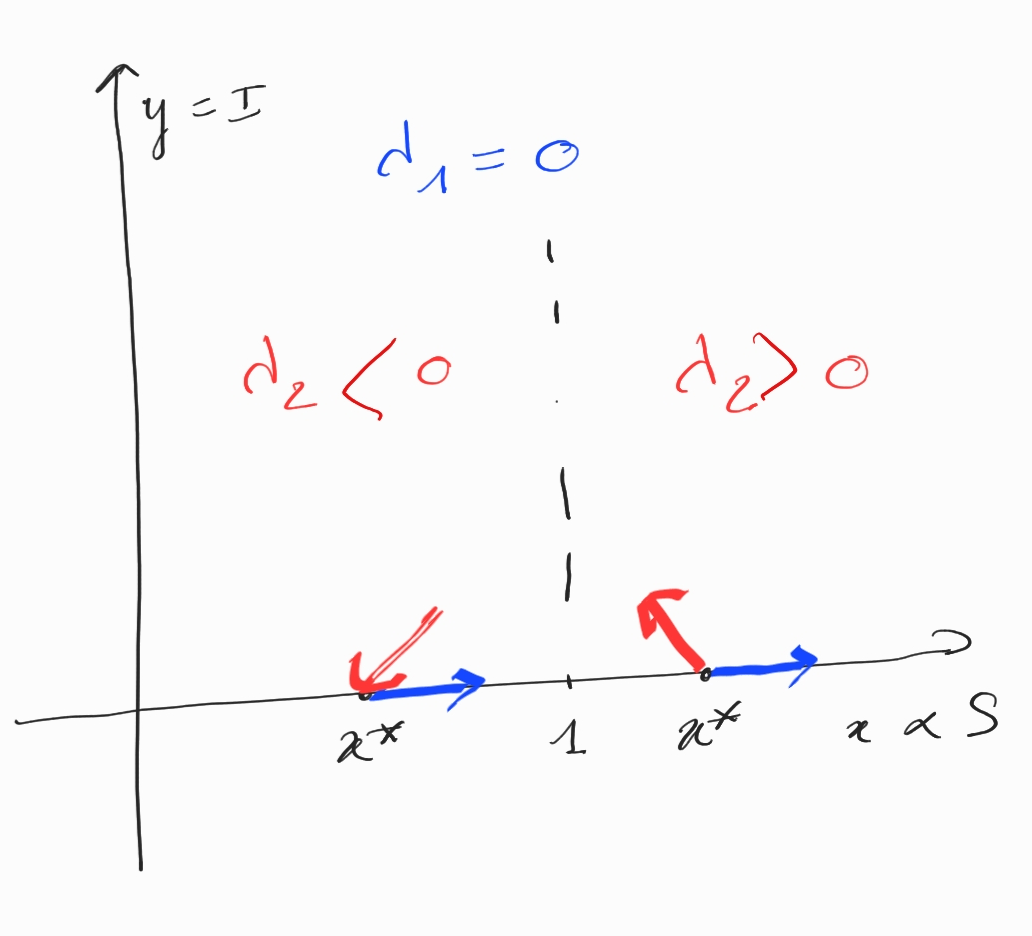
\includegraphics[width=.5\textwidth, trim=0 4 0 0, clip=]{EtudeModeleSIR}
$$
}

La trajectoire se termine toujours en un point de coordonnées $(0, x_\infty)$ avec $x_\infty < 1$, c'est à dire avec des effectifs $(S = S_\infty, I = I_\infty = 0, R_\infty = N - S_\infty)$, où $N$ est la taille constante de la population. De plus $S_\infty < a/r$ puisque $x_\infty < 1$).

\dessin{
$$
\begin{tabular}{ccc}
  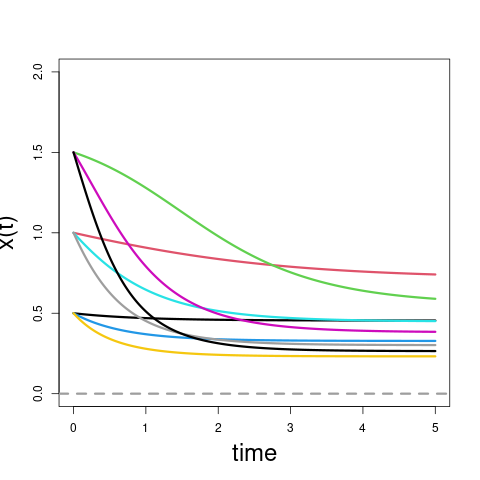
\includegraphics[width=.3\textwidth]{SIR-x} &
  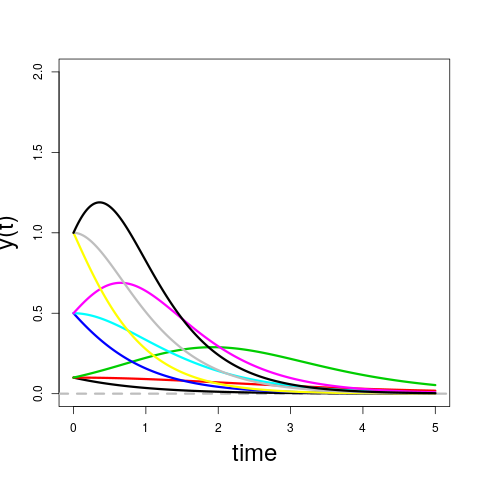
\includegraphics[width=.3\textwidth]{SIR-y} &
  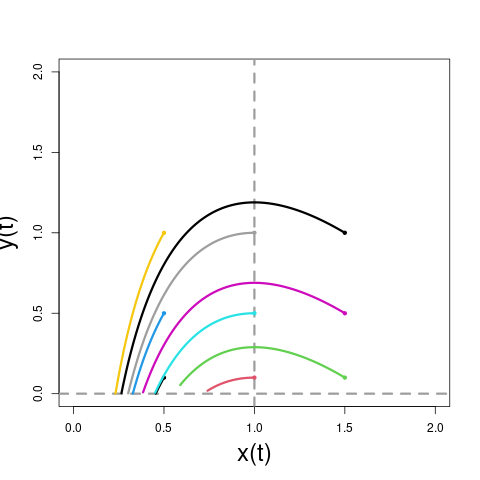
\includegraphics[width=.3\textwidth]{SIR-xy} 
\end{tabular}
$$
}

%-------------------------------------------------------------------------------
\paragraph*{Devenir de la population.}
On veut connaître les valeurs finales $(S_\infty, 0, R_\infty = N - S_\infty)$ partant d'un point $(S_0, I_0, 0)$. En reprenant la paramétrisation initiale, on remarque que, puisque
$$
\dot S = - r S I \qquad \Leftrightarrow \qquad r I = - \dot S / S,
$$
on a
$$
r \int_0^\infty I(t) \; \d t
= - \int_0^\infty \frac{\dot S(t)}{S(t)} \; \d t
= - [\log S(t)]_0^\infty
= \log \frac{S_0}{S_\infty}
$$
et que, puisque, $\dot R = aI$, on a
$$
a \int_0^\infty I(t) \; \d t
= \int_0^\infty \dot R(t) \; \d t
= [R(t)]_0^\infty
= R_\infty = N - S_\infty
$$
donc
\begin{align*}
  \frac1r \log \frac{S_0}{S_\infty} & = \frac1a (N - S_\infty) & 
  & \Leftrightarrow \qquad & 
  \log {S_0} - \log {S_\infty} & = \frac{r}a (N - S_\infty) \\
  \Leftrightarrow \qquad
  \log S_0  - N / \rho & = \log S_\infty - S_\infty / \rho &
  & \Leftrightarrow \qquad &
  S_0 e^{- N / \rho}& = S_\infty e^{- S_\infty/\rho} 
\end{align*}
pour $\rho = r/a$. On a donc
$$
f(S_\infty) = S_0 e^{- N / \rho}
\qquad \text{avec } f(x) = x e^{-x/\rho}.
$$
La fonction $f$ est nulle en 0 et $+\infty$, et sa dérivée $f'(x) = e^{-x/\rho}(1 - x/\rho)$ est positive de 0 à $\rho$, puis négative.
\dessin{
$$
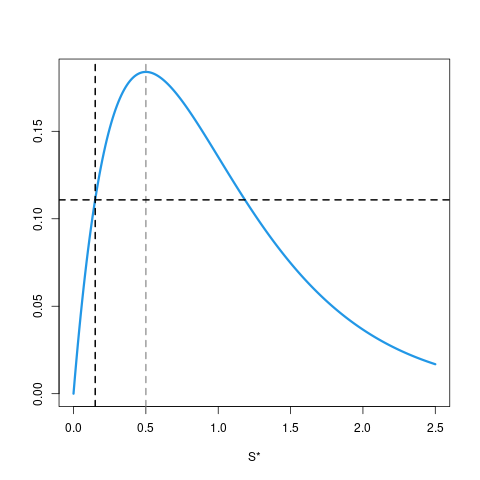
\includegraphics[width=.5\textwidth, trim=0 40 0 0, clip=]{SIR-finalState} 
$$
}
Puisqu'on sait que $x_\infty  < 1$, on a $S_\infty < \rho$ : $S_\infty$ est donné par la plus petite valeur pour laquelle $f(x)$ vaut $S_0 e^{- N / \rho}$.

On peut vértifier que cette valeur existe bien en posant $C_0 = N - S_0$, on a
$$
0 < S_0 e^{-N/\rho} = e^{-c_0/\rho} S_0 e^{-s_0 / \rho}  = e^{-c_0/\rho} f(S_0) \leq f(S_0)
$$
(puisque $e^{-c_0/\rho} \leq 1$). La valeur $S_0 e^{-N/\rho}$ est donc bien atteinte par la fonction $f$.


%-------------------------------------------------------------------------------
\chapter{Probabilités}
\minitoc
%-------------------------------------------------------------------------------
\newpage \progres{
Rappel cours 6 :
\begin{itemize}
  \item Fin EDO et systèmes dynamiques
  \item TD fonctions de plusieurs variables + EDO \& syst. synamiques
\end{itemize}
Programme cours 7 :
\begin{itemize}
  \item Dernier chapitre : probabilités (procesus)
  \item Chaînes de Makov
  \item Distribution stationnaire / comportement en temps long
\end{itemize}
}

%-------------------------------------------------------------------------------
%-------------------------------------------------------------------------------
\section{Chaînes de Markov}  \label{sec:Proba-Markov}
%-------------------------------------------------------------------------------

\newcommand{\cM}{{chaîne de Markov}\xspace}
\newcommand{\CM}{{Chaîne de Markov}\xspace}
\newcommand{\per}{\text{per}}

\todo{Trouver un exemple simple de \cM servant de fil rouge.}

\paragraph*{Objectif.}
Etudier une suite de variable aléatoires $(X_0, X_1, \dots X_n, \dots)$ non indépendantes. L'indice $n$ se réfère souvent à un temps et une telle suite est alors appelées {\em processus stochastique} à temps discert ou {\em chaîne}. % On note alors $X = (X_t)_{t \geq 0}$.

\bigskip
On suppose ici que les variables $X_n$ sont toutes à valeurs dans un même ensemble $\Ecal$ fini ou dénombrable.

%-------------------------------------------------------------------------------
\subsection{Définitions et premières propriétés}  
%-------------------------------------------------------------------------------

%-------------------------------------------------------------------------------
\subsubsection{Hypothèse de Markov}

\begin{definition}[\CM]
  $X$ est une \cM si
  $$
  \Pr\{X_{n+1} = x_{n+1} \mid X_0 = x_0, X_1 = x_1, \dots X_n = x_n\} 
  = 
  \Pr\{X_{n+1} = x_{n+1} \mid X_n = x_n\}.
  $$
\end{definition}

\begin{proposition} \label{prop:loiConditionnalleEtatInitial}
  Si $X$ est un \cM, alors
  $$
  \Pr\{X_{n+1} = k \mid X_0 = i, X_n = j\} 
  = 
  \Pr\{X_{n+1} = k \mid X_n = j\}.
  $$
\end{proposition}

% {Démonstration de la proposition \ref{prop:loiConditionnalleEtatInitial}.}
\proof
On utilise le théorème des probabilités totales pour sommer sur toutes les valeurs intermédiaires
  \begin{align*}
    \Pr\{X_0 = i, X_n = j, X_{n+1} = k\}
    & = \sum_{x_1, x_2, \dots x_{n-1}}
    \Pr\{X_0 = i, X_1 = x_1, \dots X_{n-1} = x_{n-1}, X_n = j, X_{n+1} = k\} \\
    & = \sum_{x_1, x_2, \dots x_{n-1}}
    \Pr\{X_0 = i, X_1 = x_1, \dots X_{n-1} = x_{n-1}, X_n = j, X_{n+1} = k\} \\
    & = \sum_{x_1, x_2, \dots x_{n-1}}
    \Pr\{X_{n+1} = k \mid X_0 = i, X_1 = x_1, \dots X_{n-1} = x_{n-1}, X_n = j\} \\
    & \qquad \times \Pr\{X_0 = i, X_1 = x_1, \dots X_{n-1} = x_{n-1}, X_n = j\} \\
    & = \Pr\{X_{n+1} = k \mid X_n = j\} \\
    & \qquad \times \sum_{x_1, x_2, \dots x_{n-1}} \Pr\{X_0 = i, X_1 = x_1, \dots X_{n-1} = x_{n-1}, X_n = j\} \\
    & = \Pr\{X_{n+1} = k \mid X_n = j\} \Pr\{X_0 = i, X_n = j\}.
  \end{align*}
  Il suffit alors de diviser par $\Pr\{X_0 = i, X_n = j\}$ des deux côtés. 
\eproof

%-------------------------------------------------------------------------------
\subsubsection{Matrice de transition}

\begin{definition}[\CM homogène]
  Une \cM $X$ est homogène si
  $$
  \forall n \geq 1: \qquad 
  \Pr\{X_{n+1} = j \mid X_n = i\} = p_{ij} 
  \qquad (\text{indépendant de $n$}).
  $$
\end{definition}

\begin{definition}[Probabilité et matrice de transition]
  Soit $X$ un \cM homogène, on appelle probabilités de transition les probabilités :
  $$
  p_{ij} = \Pr\{X_1 = j \mid X_0 = i\}, \qquad \forall i, j \in \Ecal.
  $$
  On appelle de plus matrice de transition la matrice $P$ de terme général $p_{ij}$:
  $$
  P = [p_{ij}].
  $$
\end{definition}

\remarks
\begin{enumerate}
  \item On utilise la notation matricielle même si $\Ecal$ est infini (mais dénombrable).
  \item On rappelle que $P$ est une {\em matrice stochastique} : 
  $$
  \forall i \in \Ecal: \qquad \sum_{j \in \Ecal} p_{ij} = 1.
  $$
  En conséquence, chaque ligne $(p_{ij})_{j \in \Ecal}$ de $P$ définie une loi de probabilité.
\end{enumerate}

\begin{definition}[Transition de $n$ étapes]
  Soit $X$ un \cM homogène, on appelle probabilités de transition en $n$ étapes les probabilités :
  $$
  p_{ij}(n) = \Pr\{X_n = j \mid X_0 = i\}, \qquad \forall i, j \in \Ecal.  
  $$
\end{definition}

\begin{proposition} \label{prop:transitionNEtapes}
  Soit $X$ une \cM homogène, les probabilités $p_{ij}(n)$ sont les termes généraux de la matrice $P^n$ : 
  $$
  p_{ij}(n) = [P^n]_{ij}.
  $$
\end{proposition}

% {Démontration de la proposition \ref{prop:transitionNEtapes}.}
\proof
Le démonstration se fait par récurrence en supposant la propriété vraie au rang $n$. Il suffit alors de sommer sur tous les états précédents possibles : 
\begin{align*}
  p_{ik}(n+1) 
  & = \Pr\{X_{n+1} = k \mid X_0=i\} \\
  & = \sum_{k \in \Ecal} \Pr\{X_{n+1} = k, X_n = j \mid X_0=i\} \\
  & = \sum_{k \in \Ecal} \Pr\{X_n = j \mid X_0=i\} \; \Pr\{X_{n+1} = k \mid X_n = j, X_0=i\} \\
  & = \sum_{k \in \Ecal} \Pr\{X_n = j \mid X_0=i\} \; \Pr\{X_{n+1} = k \mid X_n = j\} \qquad (\text{cf exercice précédent})\\
  & = \sum_{k \in \Ecal} p_{ij}(n) \; p_{jk} = \sum_{k \in \Ecal} [P^n]_{ij} p_{jk} = [P^{n+1}]_{ik}.
\end{align*}
\eproof

\remark
La loi d'une \cM homogène $X$ est donc entièrement spécifiée par
\begin{itemize}
  \item sa matrice de transition $P$ et
  \item la distribution de sa valeur initiale $X_0$.
\end{itemize}

\paragraph*{Notation.}
Dans la suite on notera $\Pr_\mu$ la loi d'une \cM $X$
\begin{itemize}
  \item de distribution initiale $\mu$: $X_0 \sim \mu$ et
  \item de matrice de transition $P$.
\end{itemize}
On notera notamment $\Pr_i$ la loi de $X$ si $x_0 = i$, c'est à dire
$$
\Pr_\mu = \sum_{i \in \Ecal} \mu_i \Pr_i.
$$

\remark
On peut identifier la distribution $\mu$ à un vecteur ligne $\mu^\top$ (éventuellement infini). On peut alors écrire
$$
\Pr_\mu\{X_n = j\} 
= \sum_{i \in \Ecal} \Pr\{X_0 = i\} \Pr\{X_n = j \mid X_0 = i\}
= \sum_{i \in \Ecal} \mu_i p_{ij}(n)
= \sum_{i \in \Ecal} \mu_i [P^n]_{ij}
= [\mu^\top P^n]_j.
$$

%-------------------------------------------------------------------------------
\subsection{Distribution stationnaire}  
%-------------------------------------------------------------------------------

\begin{definition}
  Une distribution $\nu$ sur $\Ecal$ est dite \emph{invariante} pour la \cM $X$ si 
  $$
  \nu^\top P = \nu^\top.
  $$
\end{definition}

Les distributions invariantes jouent pour les chaînes de Markov un rôle analogue au point stationnaires en système dynamique : une fois atteinte, la distribution reste constante. Comme pour les systèmes dynamiques, la question est alors de savoir si elles seront atteintes et à quelle condition. Pour répondre à cette question, il nous faut d'abord définir une notion de convergence pour des distributions.

\begin{definition}[Convergence en loi]
  Une suite de v.a. $(Y_n)_{n \geq 0}$ à valeur dans $\Ecal$ converge en loi vers une distribution $\nu$ sur $\Ecal$ :
  $$
  (Y_n)_{n \geq 0} \overset{\Lcal}{\underset{n \to \infty}{\longrightarrow}} \nu
  $$
  si
  $$
  \forall i \in \Ecal: \qquad \lim_{n \to \infty} \Pr\{Y_n = i\} = \nu_i.
  $$
\end{definition}

\begin{proposition} \label{prop:convergenceEsperance}
  Si
  $$
  (Y_n)_{n \geq 0} \overset{\Lcal}{\underset{n \to \infty}{\longrightarrow}} \nu
  $$
  alors, pour toute fonction $f : \Ecal \mapsto \Rbb$ bornée, 
  $$
  \lim_{n \to \infty} \Esp(f(Y_n)) = \sum_{i \in \Ecal} \nu_i f(i)
  $$
  (c'est à dire $\lim_{n \to \infty} \Esp(f(Y_n)) = \Esp(f(Y))$ pour $Y \sim \nu$).
\end{proposition}

% {Démonstration de la proposition \ref{prop:convergenceEsperance}.}
\proof 
\begin{description}
  \item[$\Ecal$ fini :] la démonstration vient en intervertissant la somme et la limite (puisque $\Ecal$ est fini) : 
  $$
  \lim_{n \to \infty} \Esp(f(Y_n)) 
  = \lim_{n \to \infty} \left(\sum_{i \in \Ecal} \Pr\{Y_n = i\} f(i)\right)
  = \sum_{i \in \Ecal} \left(\lim_{n \to \infty} \Pr\{Y_n = i\} \right) f(i) 
  = \sum_{i \in \Ecal} \nu_i f(i).
  $$
  \item[$\Ecal$ infini dénombrable :] sans perte de généralité, on identifie $\Ecal$ à $\Nbb$. Comme pour le cas fini, on montre facilement que, pour tout $i$,
  $$
  \lim_{n \to \infty} \Pr\{Y_n \leq i\} = \Pr\{Y \leq i\}
  \qquad \Rightarrow \qquad 
  \lim_{n \to \infty} \Pr\{Y_n > i\} = \Pr\{Y > i\}.
  $$
  On note $M$ un majorant de $f$ (qui est bornée). On peut écrire que
  \begin{align*}
    \left|\Esp(f(Y_n)) - \Esp(Y)\right|
    & = \left|\sum_{j \geq 0} \Pr\{Y_n=j\} f(j) - \sum_{j \geq 0} \nu_j f(j)\right| \\
    & \leq \left|\sum_{j=0}^i \Pr\{Y_n=j\} f(j) - \sum_{j=0}^i \nu_j f(j)\right|
    + \left|\sum_{j > i} \Pr\{Y_n=j\} f(j) - \sum_{j > i} \nu_j f(j)\right| \\
%     & \leq \left|\sum_{j=0}^i \Pr\{Y_n=j\} f(j) - \sum_{j=0}^i \nu_j f(j)\right|
%     + \left|\sum_{j > i} \Pr\{Y_n=j\} f(j)\right| + \left|\sum_{j > i} \nu_j f(j)\right| \\
    & \leq M \sum_{j=0}^i \left|\Pr\{Y_n=j\} - \nu_j\right| + M \Pr\{Y_n > i\} + M \Pr\{Y > i\}.
  \end{align*}
  La suite de la preuve consiste à majorer chacun des trois termes par $\varepsilon/3M$. 
  \begin{itemize}
  \item On commence par utiliser le fait que, pour toute v.a. $U$ à valeur dans $\Nbb$, 
  $$
  \lim_{i \to \infty} \Pr\{Y_n > i\} = 0
  $$
  (puisque la somme $\sum_{n \in \Nbb} \Pr\{U = i\}$ converge). \\
  Donc, pour tout $\epsilon > 0$, il existe un $i$ et un $n_1^{(i)}$ tels que 
  \begin{align*}
  \Pr\{Y > i\} & < \epsilon / 3M, \\
  \text{et} \qquad 
  \forall n > n_1^{(i)}: \quad \Pr\{Y_n > i\} & < \epsilon / 3M.
  \end{align*}
  \item D'autre part, puisque $i$ est fini (i.e. en utilisant le résultat dans le cas fini), il existe de plus $n_2^{(i)}$ tel que 
  $$
  \forall n > n_2, \; \forall j \leq i: \quad \left|\Pr\{Y_n=j\} - \nu_j\right| < \frac\epsilon{3M(i+1)}.
  $$
  \end{itemize}
  On a donc, 
 \begin{align*}
   \forall n > \max(i, n_1^{(i)}, n_2^{(i)}): \qquad 
   \left|\Esp(f(Y_n)) - \Esp(Y)\right| \leq \frac{M\epsilon}{3M} \underset{=1}{\underbrace{\sum_{j=0}^i \frac1{i+1}}} + \frac{M\epsilon}{3M} + \frac{M\epsilon}{3M} = \epsilon.
  \end{align*}
\end{description}
\eproof

\remarks
\begin{enumerate}
\item Si $\Ecal$ est fini, la proposition \ref{prop:convergenceEsperance} nous assure par exemple que, si $(Y_n)_{n \geq 0}$ converge en loi vers $\nu$ et que $Y \sim \nu$, on a, en prenant respectivement $f(x) = x$ et $f(x) = x^2$, 
$$
\lim_{n \to \infty} \Esp(Y_n) = \Esp(Y), \qquad
\lim_{n \to \infty} \Esp(Y_n^2) = \Esp(Y^2)
$$
et, par conséquent, $\lim_{n \to \infty} \Var(Y_n) = \Var(Y)$. 
\item Pour $\Ecal$ quelconque, en prenant $f(x) = \Ibb\{x \leq u\}$, on a $\Esp(f(Y_n)) = \Pr\{Y_n \leq u\}$ et donc, pour tout $u$, 
$$
(Y_n)_{n \geq 0} \overset{\Lcal}{\rightarrow} \nu
\qquad \Rightarrow \qquad
\lim_{n \to \infty} \Pr\{Y_n \leq u\} = \Pr\{Y \leq u\}.
$$
\end{enumerate}

\begin{definition}
  Une distribution $\nu$ sur $\Ecal$ est dite \emph{stationnaire} pour la \cM $X$ si il existe une distribution $\mu$ telle que 
  $$
  \lim_{n \to \infty} \mu^\top P^n = \nu.
  $$
  C'est à dire que la \cM $X$ de transition $P$ et de distribution initiale $\mu$ converge en loi vers $\nu$.
\end{definition}

\begin{proposition} \label{prop:stationnaireInvariante}
  Une distribution $\nu$ sur $\Ecal$ est stationnaire pour la \cM $X$ ssi elle est invariante.
\end{proposition}

% {Démonstration de la proposition \ref{prop:stationnaireInvariante}.}
\proof
\begin{description}
  \item[$\Leftarrow$ :] il suffit de prendre $\mu = \nu$ pour s'assurer que $\mu^\top P^n = \nu^\top P^n = \nu$ pour tout $n$. (La \cM est alors dite {\em stationnaire}.)
  \item[$\Rightarrow$ :] si $\nu$ est stationnaire alors il existe $\mu$ telle que $\mu^\top P^n$ converge vers $\nu$ (i.e. $\lim_{n \to \infty} [\mu^\top P]_j = \nu_j$), ce qui implique que $\mu^\top P^{n+1}$ converge également vers $\nu$, i.e.
  $$
  \lim_{n \to \infty} [\mu^\top P^{n+1}]_j = \nu_j.
  $$
  Or, par l'exercice précédent, en prenant $f(i) = p_{ij}$, on a
  $$
  \lim_{n \to \infty} [\mu^\top P^{n+1}]_j
  = \lim_{n \to \infty} \sum_{i \in \Nbb} [\mu^\top P^n]_i p_{ij}
  = \sum_{i \in \Nbb} \nu_i p_{ij}
  = [\nu^\top P]_j,
  $$
  soit $\nu^\top P = \nu^\top$.
\end{description}
\eproof


% %-------------------------------------------------------------------------------
% \subsubsection{Chaîne de Markov}
% %-------------------------------------------------------------------------------
% 
% On revient maintenant aux chaînes de Markov introduites à la section \ref{sec:MatStoch} et qui seront étudiées plus en détail à la section \ref{sec:Proba-Markov}.
% 
% \begin{definition}
%   Une chaîne de Markov homogène à espace fini est une suite de variables aléatoires $\{X(n)\}_{n \geq 0}$ à valeur dans $\Xcal$ (identifié à $\{1, \dots k\}$) non indépendantes mais telles que
%   $$
%   \Pr\{X(n+1) = j \mid X(0)=x_0, X(1) = x_1) \dots X(n) = i\}
%   = \Pr\{X(n+1) = j \mid X(n) = i\}
%   = p_{ij}.
%   $$
%   La matrice $P = [p_{ij}]$ est appelée matrice de transition de la chaîne de Markov.
% \end{definition}
% 
% La matrice $P$ est une matrice stochastique car tous ses éléments sont positifs ou nuls et leur somme en ligne vaut 1 : 
% $$
% \sum_{j = 1}^k p_{ij} = 1.
% $$
% 
% \begin{proposition}
%   Soit $\mu_0$ la distribution de $X(0)$ : $\mu_{0i} = \Pr\{X(0) = i\}$ et $mu_n^{\mu_0}$ la distribution de $X(n)$ sachant la distribution initiale $\mu_0$, on a 
%   $$
%   \mu_n^{\mu_0} = \mu_0 A^n 
%   $$
% \end{proposition}
% 
% \proof
% Par récurrence, partant de $\mu_1^{\mu_0} = A \mu_0$.
% \eproof
% 
% Comme pour les modèles de dynamique des populations, le comportement de la chaîne de Markov en temps long est gouverné par par celui de $A^n$ (et par $\mu_0$).
% 
% \begin{proposition}
%   Si $A$ est diagonalisable, ses valeurs propres sont aussi les valeurs propres de $A^\top$ et les vecteurs propres de $A^\top$ sont les vecteurs lignes de $P^{-1}$.
% \end{proposition}
% 
% \proof
%   Il suffit de remarquer que, puique $A = P D P^{-1}$, on a 
%   $$
%   A^\top 
%   = (P D P^{-1})^\top 
%   = (P^{-1})^\top D^\top  P^\top
%   = (P^{-1})^\top D P^\top 
%   $$
%   donc $A^\top$ est aussi diagonalisable et possède les même valeurs propres (contenues dans $D$) que $A$. Pour les mêmes raisons, les vecteurs propres de $A^\top$ sont les vecteurs colonnes de $(P^{-1})^\top$, c'est à dire les vecteurs lignes de $P^{-1}$.
% \eproof
% 
% \remark
% Si $A$ est diagonalisable et que $u$ est un vecteur propre de $A^\top$, il existe $\lambda$ tel que
% $$
% A^\top u  = \lambda u 
% \qquad \Leftrightarrow \qquad
% (A^\top u)  = \lambda u^\top 
% \qquad \Leftrightarrow \qquad
% u^\top A  = \lambda u^\top 
% $$
% $u^\top$ est appelé vecteur propre {\em à gauche} de $A$ (les vecteurs propres précédemment définis étant donc des vecteurs propres {\em à droite}). Cette remarque est notamment utile pour étudier les matrice stochastiques.
% 
% Le théorème de Perron-Frobénius donne des conditions garantissant que la distribution $\mu_n$ converge vers le vecteur propre (à gauche) associé à la valeur propre 1, quelque soit la distribution initiale $\mu_0$. Ces propriétés seront étudiées en détail à la section \ref{sec:Proba-Markov}.
% 
% %-------------------------------------------------------------------------------
% \paragraph*{Exemple.}
% Succession d'espèces d'arbres (R. Arditi)
% \dessin{\url{TreeSpeciesMC}}

%-------------------------------------------------------------------------------
\subsection{Comportement en temps long}  
%-------------------------------------------------------------------------------

\begin{proposition} \label{prop:perronFrobeniusCM}
%[Exercice 1.1.14+]
  Si $\Ecal$ est fini, $1$ est la plus grande valeur propre en module de $P$. \\
  Si $P$ est de plus régulière, $1$ la seule valeur propre de module 1 et est d'ordre de multiplicité 1 : elle donc la valeur propre dominante de $P$.
\end{proposition}

% {Démonstration de la proposition \ref{prop:perronFrobeniusCM}.}
\proof
\begin{enumerate}
 \item On montre facilement que 1 est valeur propre de $P$ (car $P$ est stochastique), donc $\lambda_1 \geq 1$.
 \item Soit $\lambda$ une valeur propre de $P$ et $v$ un vecteur propre associé, on a $P^n v = \lambda^n v$ où $P^n$ est stochastique (voir section \ref{sec:MatStoch}), donc les coordonnées de $P^n v$ sont bornées par la plus grande coordonnée de $v$, ce qui impose que $\lambda \leq 1$, donc $\lambda_1 \leq 1$.
 \item Le fait que $P$ soit régulière assure, par le théorème \ref{thm:perronFrobenius} de Perron-Frobenius, que $\lambda_1$ est la valeur propre unique de module 1, toutes les autres ayant des modules strictement inférieurs. 
\end{enumerate}
\eproof

\remark
Le théorème \ref{thm:perronFrobenius} de Perron-Frobenius nous assure que les vecteurs propres (à gauche et à droite) associés à $\lambda_1 = 1$ ont toutes leurs coordonnées positives. On a ainsi démontré que, pour $\Ecal$ fini, si $P$ est régulière, 
\begin{itemize}
  \item elle admet une unique distribution stationnaire $\nu$ et que $\nu_i > 0$ pour tout $i \in \Ecal$, 
  \item quelque soit la distribution initiale $\mu$, $\mu P^n \to \nu$, c'est-à-dire que $X_n$ converge en loi vers $\nu$.
\end{itemize}

\progres{
Rappel cours 7 :
\begin{itemize}
  \item Chaînes de Markov
  \item Probabilités et matrice de transition
  \item Distribution invariante et stationnaire
  \item Comportement en temps long et convergence vers une distribution stationnaire (redonner la proposition \ref{prop:perronFrobeniusCM})
\end{itemize}
Programme cours 8 :
\begin{itemize}
  \item Communication entre états
  \item Classification des états
  \item Quelques exemples de \cM (Wright-Fisher)
  \item Processus de branchement
\end{itemize}
}

\begin{definition}[Communication entre états]
  On dit qu'il existe un {\em chemin de $i$ vers $j$} (ou que $j$ est {\em accessible depuis $i$}) s'il existe $n \geq 0: p_{ij}(n) > 0$. \\
  S'il existe une chemin de $i$ vers $j$ et un chemin de $j$ vers $i$, on dit que $i$ et $j$ communique et on note $i \sim j$.
\end{definition}


\begin{proposition}  \label{prop:communicationEquivalence}
  La relation de communication 
  $$
  \Rcal(i, j) \Leftrightarrow \{\text{$i$ communique avec $j$}\}
  $$
  est une relation d'équivalence. 
\end{proposition}

\proof
$\Rcal$ vérifie les trois condition d'une relation d'équivalence : 
\begin{itemize}
  \item reflexivité: $\forall i \in \Ecal: \Rcal(i, i)$ en prenant $n = 0$, soit $P^0 = I$ ;
  \item symétrie : $\forall i, j \in \Ecal: \Rcal(i, j) \Rightarrow \Rcal(j, i)$ ;
  \item transitivité : $\forall i, j, k \in \Ecal: \Rcal(i, j), \Rcal(j, k) \Rightarrow \Rcal(i, k)$.
\end{itemize}
\eproof

\remark
$\Rcal$ définit donc des classes d'équivalences $\Ccal_1, \Ccal_2, \dots $, qui constituent une partition de $E$:
$$
\cup_{k \geq 0} \Ccal_k = \Ecal, \qquad \forall j \neq k: \quad \Ccal_j \cap \Ccal_k = \varnothing.
$$
Les classes $\Ccal_k$ sont appelées {\em classes de communication}.

\begin{definition}
  Une \cM est dite {\em irréductible} si elle admet une seule classe de communication.
\end{definition}

\remark
L'hypothèse de régularité de $P$ implique que $X$ est irréductible (puisque $\exists n: P^n > 0$) mais pas l'inverse, puisque les états peuvent tous communiquer pour des $n$ différents.


%-------------------------------------------------------------------------------
\exemple{[$\Ecal = \{0, 1\}$.]
On considère la \cM $X$ de matrice de transition 
$$
P = \left[\begin{array}{ccc}
      1 - p & & p \\
      q & & 1 - q 
    \end{array}\right]
$$
\begin{description}
  \item[$p = q = 0$ :] alors $P = I$ et toute distribution est stationnaire, mais $P$ n'est pas régulière et la loi de $X_n$ est la même que celle de $X_0$.
  \item[$0 < p, q < 1$ :] alors la seule distribution stationnaire est 
  $$
  \nu = \left[ \frac{q}{p+q} \;  \frac{p}{p+q} \right],
  $$
  et comme $P$ est régulière, $X_n$ converge en loi vers $\nu$ quelque soit la distribution initiale $\mu$.
  \item[$p = q = 1$ :] alors la seule distribution stationnaire est 
  $$
  \nu = \left[ \frac12 \;  \frac12 \right],
  $$
  mais comme $P$ n'est pas régulière, $X_n$ ne converge pas nécessairement vers $\nu$. \\En fait $X_n$ alterne entre les états $0$ et $1$ et ne converge en loi vers $\nu$ que si $\mu = \nu$ (et alors $X_n \sim \nu, \forall n$). Si $X_0 = 0$ ou $X_0 = 1$ (ou $\mu \neq \nu$), alors $X_n$ ne converge pas du tout.
\end{description}
}
 
%-------------------------------------------------------------------------------
\subsection{Classification des états}  
%-------------------------------------------------------------------------------

% Loi du nombre de visites d’un état transient, théorème ergodique pour les chaînes récurrentes à espace d’états fini. 

On cherche maintenant à établir une classification des comportements possibles d'une \cM. La notion de temps de retour est centrale pour effectuer cette description.

\begin{definition}[Temps de retour]
  Le temps de retour dans l'état $i$ est défini pour $X_0 = i$ par
  $$
  T_i := \min\{n : X_n = i\} \leq + \infty \qquad (\text{i.e. possiblement } + \infty).
  $$
\end{definition}

\begin{definition}[\'Etat récurrent]
  L'état $i$ est dit {\em récurrent} si $\Pr_i\{T_i < + \infty\} = 1$. Dans le cas contraire, $i$ est dit {\em transient}. \\
  L'état $i$ est dit {\em récurrent positif} s'il est récurrent et $\Esp(T_i) < + \infty$. Dans le cas contraire il est dit récurrent nul.
\end{definition}

% \begin{definition}[\'Etat transient]
%   L'état $i$ est transient si $\Pr_i\{T_i < + \infty\} = 1$.
% \end{definition}

\begin{definition}[Période d'un état]
  La période de l'état $i$ est le plus grand diviseur commun des temps de retour possible dans l'état :
  $$
  \per(i) = PGCD\{n: p_{ii}(n) > 0\}.
  $$
  Une \cM est dite {\em apériodique} si $\per(i) = 1$ pour tout $i$.
\end{definition}

\dessin{Dessiner qques graphes de transition de \cM avec ou sans période.}

\begin{proposition}[Cas $\Ecal$ fini]
  Si $\Ecal$ est fini, il n'existe pas d'état récurrent nul et il existe au moins un état récurrent positif.
\end{proposition}

\proof Non démontré. \eproof

\begin{proposition}
  Tous les états d'une même classe de communication sont de même nature (récurrent positif, récurrent nul, transient). \\
  Si $\Ecal$ est fini et $X$ irréductible, son unique classe de communication est récurrente positive.
\end{proposition}

%-------------------------------------------------------------------------------
\exemple{[Modèle de Wright-Fisher]
  Le modèle de Wright-Fisher est un modèle classique en génétique des populations. On y considère les générations successive d'une population de taille fixe $N$ de reproduction non-sexuée. Parmi ces $N$ individus, $x$ sont porteurs de l'allèle $A$ (et $N-x$ sont porteurs de l'allèle $B$) d'un gène donné. On s'intéresse au processus $X = (X_n)_{n \geq 0}$ où
  $$
  X_n = \text{nombre d'individus porteurs de l'allèle $A$ à la génération $n$}
  $$
  en supposant que, à chaque génération, chacun de $N$ nouveaux individus tire indépendamment et uniformément son parent parmi la génération précédente (et hérite de son allèle). 
  \begin{description}
    \item[Probabilité de transition.] Un individu de la génération $n+1$ a donc un probabilité $x_n/N$ de porter l'allèle $A$. Les individus étant indépendant, on a
    $$
    (X_{n+1} \mid X_n=x) \sim \Bcal(N, x/N).
    $$
    La probabilité de transition vaut donc
    $$
    p_{ij} = \binom{N}{j} \left(\frac{i}N\right)^j \left(\frac{N-i}N\right)^{N-j}.
    $$
    \item[Classification des états.] Les états se répartissent en trois classes
    $$
    \Ccal_1 = \{0\}, \qquad \Ccal_2 = \{N\}, \qquad \Ccal_3 = \{1, \dots, N-1\}.
    $$
    Les classes $\Ccal_1$ et $\Ccal_2$ sont absorantes. La \cM finira nécessairement par atteindre l'une d'entre elles, $\Ccal_3$ est donc transiente.
    \item[Probabilité de fixation.] Il reste à savoir quel état absorbant sera atteint en premier. Notons $q_i$ la probabilité d'atteindre l'état $x=N$ (avant l'état $x=0$) en partant de $X_0 = i$. On a 
    $$
    q_0 = 0, \qquad q_N = 1.
    $$
    Pour les autres valeurs de $i$, en décomposant les chemins allant de $i$ à $N$ : 
    \begin{itemize}
      \item soit $i \to N$ en une étape, 
      \item soit $i \to j \notin \{0, N\}$ en une étape, puis $j \to N$ en un nombre indéterminé d'étapes, 
    \end{itemize}
    on peut écrire que :
    $$
    q_i = \sum_{j=1}^{N-1} p_{ij} q_j + p_{iN}
    $$
    et vérifier que $q_i = i/N$ satisfait cette équation, en effet :
    \begin{align*}
      \sum_{j=1}^{N-1} p_{ij} \frac{j}N + p_{iN}
      & = \sum_{j=1}^{N-1} \binom{N}{j} \left(\frac{i}N\right)^j \left(\frac{N-i} N\right)^{N-j} \frac{j}N + \left(\frac{i}N\right)^N \\
%       & = \binom{N}{j} \left(\frac{N-i} N\right)^N \sum_{j=1}^{N-1} \left(\frac{i}N\right)^j \left(\frac{N-i} N\right)^{-j} \frac{j}N + \left(\frac{i}N\right)^N \\
      & = \sum_{j=1}^{N-1} \binom{N-1}{j-1} \left(\frac{i}N\right)^j \left(\frac{N-i} N\right)^{N-j} + \left(\frac{i}N\right)^N \\
      & = \frac{i}N \sum_{k=0}^{N-2} \binom{N-1}{k} \left(\frac{i}N\right)^k \left(\frac{N-i} N\right)^{N-1-k} + \left(\frac{i}N\right)^N \\
      & = \frac{i}N \left[\left(\frac{i}N + \frac{N-i}N\right)^{N-1} - \left(\frac{i}N\right)^{N-1}\right] + \left(\frac{i}N\right)^N \\
      & = i/N.
    \end{align*}
    (On ne démontre pas ici que $q_i = i/N$ est l'unique solution.) La probabilité de fixation de l'allèle $A$ est donc $i/N$ (et celle de l'allèle $B$ est $(N-i)/N$).
  \end{description}
  
}

%-------------------------------------------------------------------------------
\exemple{[Marche aléatoire sur $\Zbb$]
  On considère la \cM $X$ à valeur dans $\Ecal = \Zbb$, de probabilités de transition
  $$
  p_{i, j} = \left\{\begin{array}{rl}
                    p & \text{si } j = i+1, \\
                    1 - p & \text{si } j = i-1, \\
                    0 & \text{sinon.}
                    \end{array}\right.
  $$
  \begin{description}
    \item[$p = 0$ ou $p = 1$:] chaque singleton constitue une classe transiente (la \cM y passe une fois et une seule).
    %
    \item[$p \in (0, 1)$:] $X$ est irréductible ($\Zbb$ forme une unique classe de communication). En notant $E_n$ le déplacement $X_n - X_{n-1}$, on voit que les $E_n$ sont iid à valeur dans $\{-1, +1\}$ et de loi
    $$
    \Pr\{E_n = 1\} = p = 1 - \Pr\{E_n = -1\}.
    $$
    On a notamment
    \begin{align*}
      \Esp(E_n) & = n (2p - 1) =: m, \\
      \Var(E_n) & = \Esp(E_n^2) - (2p - 1)^2 = 1 - (4p^2 - 4p + 1) = 4p(1-p) =: s^2.
    \end{align*}
    Puisque
    $$
    X_n = X_0 + \sum_{i=1}^n X_i,
    $$
    la loi des grands nombre nous assure que 
    $$
    \lim_{n \to \infty} \frac{X_n}n = \lim_{n \to \infty} \left(\frac{X_0}n + \frac1n \sum_{i=1}^n X_i\right) = m.
    $$
    Plus précisémment encore, le théorème central limite nous assure (puisque $X_0 /n \to 0$) que
    $$
    \frac{\sqrt{n}}{s}\left(\frac{X_n}n - m\right) \overset{\Lcal}\rightarrow \Ncal(0, 1),
    $$
    c'est-à-dire que
    $$
    \lim_{n \to \infty} \Pr\left\{\frac{\sqrt{n}}{s}\left(\frac{X_n}n - m\right) \in [a, b]\right\} = \Pr\{\Ncal(0, 1) \in [a, b]\}.
    $$
    \item[$p \in (0, 1)$ et $p \neq 1/2$:] alors $\Esp(X_n) = nm$ et
    $$
    \frac{\sqrt{n}}{s}\left(\frac{X_n}n - m\right) \in [a, b]
    \qquad \Leftrightarrow \qquad
    X_n \in [nm + \sqrt{n}as, nm + \sqrt{n}bs].
    $$
    La trajectoire est dite {\em balistique} (elle s'écarte de son origine à vitesse linéaire) et son écart type $\sqrt{\Var(X)}$ croît seulement en $\sqrt{n}$. $X_n$ tend vers $+\infty$ si $p > 1/2$ et vers $-\infty$ si $p < 1/2$ et la \cM est transiente.
    \item[$p = 1/2$:] on parle alors de marche aléatoire {\em symétrique}. Dans ce cas, $m=0$ et $s^2 = 1$, donc
    $$
    \frac{\sqrt{n}}{s}\left(\frac{X_n}n - m\right) \in [a, b]
    \qquad \Leftrightarrow \qquad
    X_n \in [\sqrt{n}a, \sqrt{n}b].
    $$
    $X_n$ si situe alors typiquement à une distance $\sqrt{n}$ de son origine. \\
    On peut montrer que $X$ est récurrente nulle : la \cM repasse un nombre infini de fois dans chaque état, mais les temps de passage sont de plus en plus espacés.
  \end{description}
  $$
  \begin{array}{cc}
    p = 1/3 & p = 1/2 \\
    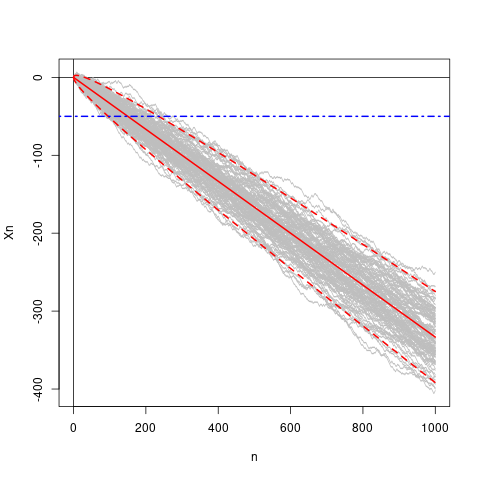
\includegraphics[width=.4\textwidth, trim=0 0 20 50, clip=]{MarcheAleatoire-p33} & 
    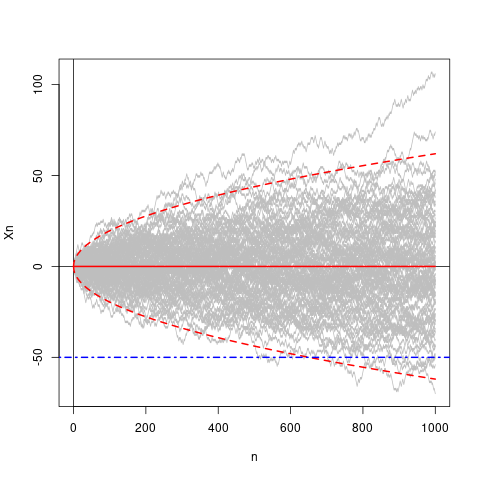
\includegraphics[width=.4\textwidth, trim=0 0 20 50, clip=]{MarcheAleatoire-p50} 
  \end{array}
  $$
}

%-------------------------------------------------------------------------------
%\subsection{Théorème ergodique}  
%-------------------------------------------------------------------------------

\begin{theorem}[Théorème ergodique]
  Si $X$ est une \cM irreductible et récurrente positive, alors 
  \begin{itemize}
   \item $X$ admet une unique distribution stationnaire $\nu$,
   \item $X$ est ergodique, c'est à dire que, pour toute distribution initiale $\mu$, on a
   $$
   \Pr_\mu\left\{\lim_{n \to \infty} \frac1n \left|\{1 \leq k \leq n: X_k = i\}\right| = \nu_i\right\} = 1,
   $$
   \item si de plus $X$ est apériodique alors $X$ converge en distribution vers $\nu$ : 
   $$
   \lim_{n \to \infty} \Pr_\mu\{X_n = i\} = \nu_i.
   $$
  \end{itemize}
\end{theorem}

\remarks
\begin{enumerate}
 \item Ce théorème est plus fort que la convergence en loi car il assure que la trajectoire de $X = (X_n)_{n \geq 0}$ elle même passe par chaque état $i$ un nombre de fois proportionnelle à $\nu_i$.
 \item La convergence en loi n'est garantie que dans le cas apériodique.
\end{enumerate}


%-------------------------------------------------------------------------------
\exemple{[$\Ecal = \{0, 1\}$]
\begin{description}
  \item[$p = q = 0$ :] la chaîne possède 2 classes récurrente ($\{0\}$ et $\{1\}$). Elle reste en fait constante et toute mesure $\nu$ est invariante.
  \item[$p = 0$ et $q \neq 0$ :] la chaîne possède une classe récurrente ($\{0\}$) et une classe transiente ($\{1\}$). La chaîne est 'absorbée' par l'état $0$ en un temps fini et la seule distribution invariante est $\nu = [1 \; 0]$.
  \item[$p = q = 1$ :] la chaîne est irréductible (on vérifie que $P^2 = I$) et récurrente positive, donc elle est ergodique (chaque état est visité la moitié du temps) mais elle est périodique et ne converge pas en loi.
  \item[$p + q = 1$ et $pq < 1$:] la chaîne est irréductible, récurrente positive et apériodique donc elle est ergodique et converge en loi vers $\nu$.
\end{description}
}


\newpage %-------------------------------------------------------------------------------
%-------------------------------------------------------------------------------
\section{Processus de branchement} \label{sec:Proba-Branchement}
%-------------------------------------------------------------------------------

%-------------------------------------------------------------------------------
\paragraph*{Processus de (Bienaymé-)Galton-Watson.}
On suit une population au cours des générations. A chaque génération, chaque individu peut avoir des descendants, qui peuvent avoir eux-même des descendants, etc. On constitue ainsi un processus de branchement qui reflète la généalogie des individus.

Si on part d'un seul individu, et qu'on note $X_{0, 1}$ le nombre de ses descendants, et $X_{1, 1}$, $X_{1, 2}$, \dots le nombre de descendants de chacun de ces descendants, on voit que la taille de la population vaut successivement
\begin{align*}
  Z_1 & = X_{0, 1}, &
  Z_2 & = \sum_{i=1}^{Z_1} X_{1, i}, &
  Z_3 & = \sum_{i=1}^{Z_2} X_{2, i}, &
  \dots
\end{align*}

%-------------------------------------------------------------------------------
\subsection{Fonction génératrice des probabilités} 
%-------------------------------------------------------------------------------

Les fonctions génératrices (il en existe plusieurs) permettent de manupuler facilement des combinaisons (notamment des sommes) de variables aléatoires.

\begin{definition}[Fonction génératrice]
  Soit $X$ une variable aléatoire positive. On note $f_X$ sa {\em fonction génératrice des probabilités} (= '{\em pgf}') définie comme
  $$
  \begin{array}{rrcl}
    f_X : & [0, 1] & \mapsto & [0, 1] \\
      & s & \to & f_X(s) = \Esp\left(s^X\right).
  \end{array}
  $$
\end{definition}

\remark
On voit facilement que $f_X(1) = 1$ et que $f_X$ est monotone croissante.

%-------------------------------------------------------------------------------
\paragraph*{Fonction génératrices de quelques lois de probabilités.}
\begin{description}
  \item[Bernoulli:] si $X \sim \Bcal(p)$ 
  $$
  f_X(s) = (1-p) s^0 + p s^1 = 1 - p + p s.
  $$
  Notamment, si $p = 1$, $f_X(s) = s$.
  \item[Binomiale:] si $X \sim \Bcal(n, p)$
  $$
  f_X(s) = \sum_{k=0}^n {{n}\choose{k}} (1-p)^{n-k} (ps)^k = (1 - p + ps)^n.
  $$
  \item[Géométrique:] si $X \sim \Gcal(a)$ ($\Pr\{X = k\} = (1-a) a^k$ pour $k \geq 0$)
  $$
  f_X(s) = (1-a) \sum_{k=0}^n (as)^k = \frac{1-a}{1 - as}.
  $$
  \item[Poisson:] si $X \sim \Pcal(\lambda)$
  $$
  f_X(s) = e^{-\lambda} \sum_{k\geq0} (\lambda s)^k / (k!) = e^{-\lambda} e^{\lambda s} = \exp(\lambda(s-1)).
  $$
\end{description}

%-------------------------------------------------------------------------------
\paragraph*{Quelques propriétés des fonctions génératrices de probabilités.}

\begin{proposition}
  La fonction génératrice $f_X$ est $C^\infty$ sur $[0, 1]$ et sa $k$-ème dérivée vaut
  \begin{align*}
    f_X^{(k)}(s) 
    & = \sum_{n \geq k} \Pr\{X = n\} n(n-1)  \dots (n-k+1) s^{X-k} \\
    & = \Esp(X (X-1) \dots (X-k+1) s^{X-k})
  \end{align*}
\end{proposition}

\proof
  $C^\infty$ non démontré. Formule de $f_X^{(k)}(s)$ directe comme dérivées successives de $s^n$.
\eproof

\begin{corollary}
  En conséquence, on a
  \begin{align*}
    \forall k \geq 0: \quad \Pr\{X = k\} & = f_X^{(k)}(0) / (k!), \\
    \Esp(X) & = f'_X(1), &
    \Esp(X(X-1)) & = f''_X(1).
  \end{align*}
\end{corollary}

\proof 
Directe.
\eproof.

\remarks
\begin{enumerate}
  \item Le corollaire justifie le nom de 'fonction génératrice des probabilités'. $F_X$ nous donne également les moments de $X$. Notamment
  \begin{align*}
    \Var(X) 
    & = \Esp(X^2) - (\Esp X)^2 \\
    & = \Esp(X(X-1) + X) - (\Esp X)^2
    = \Esp(X(X-1)) + \Esp X - (\Esp X)^2 \\
    & = f''_X(1) + f'_X(1)(1 - f'_X(1)). 
  \end{align*}
  \item En fait, la fonction génératrice caractérise complètement la loi de la variable $X$. Elle permet également d'assurer la convergence en loi.
\end{enumerate}

%-------------------------------------------------------------------------------
\progres{
Rappel cours 8 :
\begin{itemize}
  \item Fin chaînes de Markov, processus de Wright-Fisher, marche aléatoire
  \item Processus de branchement
  \item Fonction génératrice
\end{itemize}
Programme cours 9 :
\begin{itemize}
  \item Processus de Galton-Watson
  \item TD chaînes de Makov, processus de branchement
\end{itemize}
}

%-------------------------------------------------------------------------------
\begin{proposition}[Convergence de la fonction génératrice]
  Soient $(X_n)_{n \geq 0}$ une suite de variables aléatoires positives et $X$ un variable aléatoires positives :
  $$
  (X_n)_{n \geq 0} \overset{\Lcal}{\longrightarrow} X
  \qquad \Leftrightarrow \qquad
  \forall s \in [0, 1]: \quad \lim_{n \to \infty} f_{X_n}(s) = f_X(s).
  $$
\end{proposition}

\proof Non démontrée. \eproof

\begin{proposition}[Fonction génératrice de la somme]
  Soient $X$ et $Y$ deux variables aléatoires positives indépendantes, on a
  $$
  f_{X+Y}(s) = f_X(s) \; f_Y(s).
  $$
\end{proposition}

\proof
Il suffit de partir de la définition et d'utiliser l'indépendance :
$$
f_{X+Y}(s) 
= \Esp(s^{X+Y}) = \Esp(s^X \; s^Y) = \Esp(s^X) \;  \Esp(s^Y)
= f_X(s) \; f_Y(s).
$$
\eproof

\remarks
\begin{enumerate}
  \item Une conséquence directe est que si $X_1$, $X_2$, \dots $X_n$ sont positives et iid, alors la fonction génératrice de leur somme vaut
  $$
  f_{X_1 + \dots + X_n}(s) = \left(f(X_1)\right)^n.
  $$
  \item Cette propriété donne une autre démonstration de la formule de $f_X$ pour la loi binomiale, vue comme une somme de $n$ variables de Bernoulli indépendantes.
\end{enumerate}

\begin{proposition}[Fonction génératrice d'une somme en nombre aléatoire] \label{prop:fGeneratriceSommeAleatoire}
  Soient $(X_n)_{n \geq 1}$ une suite de variables aléatoires positives iid et $N$ une variables positive indépendante, on s'intéresse à la somme des $N$ premiers éléments de la suite :
  $$
  Z = \sum_{n=1}^N X_n.
  $$
  On a 
  $$
  f_{Z}(s) = f_N \circ f_X(s).
  $$
\end{proposition}

\proof
On conditionne par $N$ :
\begin{align*}
  f_Z(s) 
  = \Esp_N \left(\Esp(e^Z \mid N) \right)
  = \Esp_N \left(f_X(s)^N \right)
  = f_N \left(f_X(s)^N \right) = f_X \circ f_X(s).
\end{align*}

\eproof

%-------------------------------------------------------------------------------
\subsection{Processus de Galton-Watson (GW)} 
%-------------------------------------------------------------------------------

On reprend une population évoluant de la façon décrite au début de la section. 
On note $Z_n$ la taille de la population à la $n$-ème génération ($n \geq 0$) et $X_{ni}$ le nombre de descendants du $i$ individu de la $n$-ème génération. 
On suppose que les $\{X_{ni})_{n \geq 0, 1 \geq i \geq Z_n}$ sont iid (et indépendants de $Z_0$).

\bigskip
La taille de la population à la génération $n+1$ est donnée par 
\begin{equation} \label{eq:recurrenceGW}
Z_{n+1} = \sum_{i = 1}^{Z_n} X_{ni}.
\end{equation}
La suite $(Z_n)_{n \geq 0}$ forme donc une \cM sur $\Nbb$, puisque $Z_{n+1}$ est donné par $Z_n$ et par les $\{X_{ni})_{1 \geq i \geq Z_n}$, qui sont indépendants du passé.

\bigskip
On s'intéresse notamment à l'événement d'extinction défini par 
$$
Ext = \{T_0 < \infty\}.
$$
et à la probabilité d'extinction partant d'une population de taille 1 : 
$$
q := \Pr_1\{Ext\}.
$$


%-------------------------------------------------------------------------------
\paragraph*{Matrice de transition.} 
On peut caractériser les probabilités de transition 
$$
p_{ij} = \Pr\{Z_{n+1} = j \mid Z_n = i\}
$$
par leur fonction génératrice. En effet, \eqref{eq:recurrenceGW} donne
$$
\Esp(s^{Z_{n+1}} \mid Z_n) = f_X^{Z_n}(s)
\qquad \Rightarrow \qquad 
\sum_{j \geq 0} p_{ij} s^j = \Esp(s^{Z_{n+1}} \mid Z_n=i) = f_X(s)^i,
$$
donc
$$
p_{ij} = \frac{\left(f_X(0)^i\right)^{(j)}}{j!}.
$$
On observe qu'il s'agit bien d'une \cM homogène (puisque la fonction génératrice ne dépend par de $n$).

%-------------------------------------------------------------------------------
\paragraph*{Classification des états.} 
\begin{itemize}
 \item L'état $\{0\}$ ne communique avec aucun autre : il constitue donc une classe à lui seul. Comme il est de plus impossible d'en sortir ($p_{00} = 1$), il est récurrent : on parle d'état absorbant.
 \item Si $\Pr\{X \geq 2\} > 0$, tous les autres états communiquent, ils constituent donc une unique classe et possède tous la même nature.
 \item On peut montrer que tous les états, hormis $\{0\}$ sont transients.
\end{itemize}

Le caractère transient des états non nuls signifie qu'ils ne sont visités qu'un nombre fini de fois, ce qui signifie que soit la \cM est absorbée en 0, soit elle part vers l'infini : 
$$
\Pr_\mu\left\{ \lim_{n \to \infty} Z_n = + \infty\right\} = 1 - \Pr_\mu\{Ext\}.
$$

%-------------------------------------------------------------------------------
\paragraph*{Extinction de la population.} 
On suppose que $f_X(0) \notin \{0, 1\}$, c'est-à-dire que 
$$
0 < \Pr\{X = 0\} < 1.
$$

\remark
$\Pr\{X = 0\} = 1$ implique une extinction immédiate de la population et $\Pr\{X = 0\} = 0$, au contraire, interdit l'extinction.

\begin{proposition}
  La probabilité d'extinction $q$ est un point fixe de la fonction génératrice de $X$ :
  $$
  q = f_X(q).
  $$
\end{proposition}

\proof
On commence par remarquer que la probabilité d'extinction partant de $k$ individus indépendants vaut
$$
\Pr_k\{Ext\} = \Pr_1\{Ext\}^k = q^k,
$$
puisqu'il faut pour cela que les $k$ populations indépendantes s'éteignent. En sommant sur toutes les tailles possibles à la première génération on a donc
$$
q 
= \Pr_1\{Ext\} 
= \sum_{k \geq 0} \Pr_1\{Z_1 = k\} \Pr_k\{Ext\}
= \sum_{k \geq 0} \Pr_1\{Z_1 = k\} q^k
= f_{Z_1}(q)
= f_X(q).
$$

\begin{proposition} \label{prop:fonctionGeneratriceZn}
  La fonction génératrice de $Z_n$ partant de $Z_0 = 1$ est
  $$
  f_{Z_n}(s) = \Esp_1(s^{Z_n}) = \underset{n \text{ fois}}{\underbrace{f_X \circ f_X \circ \dots \circ f_X}}(s).
  $$
\end{proposition}

\proof 
C'est une conséquence directe de la proposition \ref{prop:fGeneratriceSommeAleatoire} : puisque
$$
Z_n = \sum_{i=1}^{Z_{n-1}} X_{n-1, i},
$$
on a la récurrence 
\begin{equation} \label{eq:recurrenceFonctionGeneratriceGW}
f_{Z_n} = f_{Z_{n-1}} \circ f_X
\end{equation}
et la preuve se conclue en remarquant que $f_{Z_1} = f_X$, puisque $Z_0 = 1$.
\eproof

\begin{definition}
  Soit $m = \Esp(X) = f'_X(1)$ le nombre moyen de descendants. Le processus GW est dit critique si $m=1$, sous-critique si $m < 1$ et sur-critique si $m > 1$.
\end{definition}

\remarks
\begin{enumerate}
  \item La récurrence \eqref{eq:recurrenceFonctionGeneratriceGW} nous assure notamment que
  $$
  \Esp(Z_n) = m \Esp(Z_{n-1}),
  $$
  en effet
  \begin{align*}
    \Esp(Z_n) 
    = f'_{Z_n}(1) = (f_{Z_{n-1}} \circ f_X)'(1) 
    = f'_X(1) \times f'_{Z_{n-1}}\left(f_X(1)\right) 
    = m f'_{Z_{n-1}}(1) = m \Esp(Z_{n-1}).
  \end{align*}
  Notamment, partant de $Z_0 = 1$, on a $\Esp_1(Z_n) = m^n$.
  \item Dans le cas où $Z_0$ est aléatoire, de fonction génératrice $f_{Z_0}$, on obtient de la même manière
  $$
  f_{Z_n} =  f_{Z_0} \circ \underset{n \text{ fois}}{\underbrace{f_X \circ f_X \circ \dots \circ f_X}}.
  $$
\end{enumerate}

\begin{lemma} \label{lem:GWnombrePointsFixes}
  Si $f_X(0) > 0$, $f_X$ admet pour points fixes dans $[0, 1]$
  \begin{align*}
    \{s = 1\} & \text{ si } m \leq 1, &
    \{0 < s_1 < 1, s_2=1\} & \text{ si } m > 1.
  \end{align*}
\end{lemma}

\proof
Nous allons montrer que la position du nombre moyen de descendants $m$ par rapport à 1 contrôle le nombre de points fixes de $f_X$.
Pour cela, on distingue les deux cas $\Pr\{X\geq 2\} = 0$ ou $\Pr\{X\geq 2\} > 0$.
\begin{itemize}
  \item Si $\Pr\{X\geq 2\} = 0$, alors $X \in \{0, 1\}$, donc c'est une variable de Bernoulli $\Bcal(m)$ et $f_X(s)$ est linéaire, de pente $m \leq 1$. $f_X$ ne croise donc la première bissectrice qu'en $s = 1$.
  \item Si $\Pr\{X\geq 2\} > 0$, alors
  \begin{align*}
  f'_X(s) 
  & = \Esp(X s^{X-1}) 
  = s^{-1} \Esp(X s^X) > 0 
  & & \text{pour} \quad s > 0, 
  \\
  f''_X(s) 
  & = \Esp(X(X-1) s^{X-2}) \\
  & = \sum_{x \geq 2} x (x-1) s^x 
  = \sum_{x \geq 0} (x+2) (x+1) s^x 
  > 0 
  & & \text{pour} \quad 0 < s \leq 1.
  \end{align*}
  La fonction $f_X$ est donc monotone croissante sur $(0, 1]$ et strictement convexe sur $(0, 1]$ avec $f_X(0) = \Pr\{X = 0\} > 0$. Son graphe coupe donc la première bissectrice 
  \begin{itemize}
  \item en $s^* < 1$ et en 1 si $f'_X(1) = m > 1$,
  \item en 1 seulement si $f'_X(1) = m \leq 1$.
  \end{itemize}
\end{itemize}
\eproof

$$
\begin{tabular}{cc}
  \begin{tabular}{l}
    \textcolor{red}{\bf --} : $m < 1$ \\ ~ \\
    \textcolor{green}{\bf --} : $m = 1$ \\ ~ \\
    \textcolor{blue}{\bf --} : $m > 1$
  \end{tabular}
  &
  \begin{tabular}{c}
  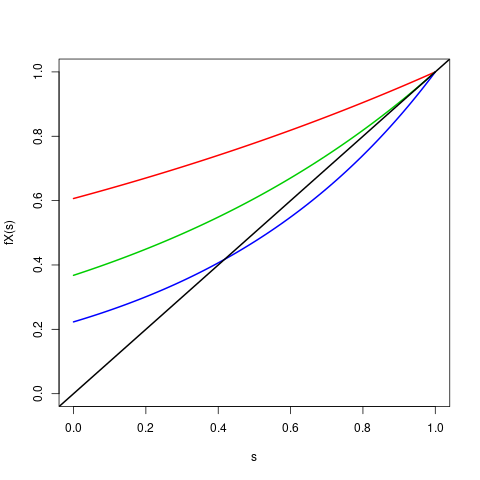
\includegraphics[width=.4\textwidth]{GaltonWatson-pgf}
  \end{tabular}
\end{tabular}
$$

\remarks
\begin{enumerate}
  \item On voit ainsi que la probabilité d'extinction vaut $q = 1$ si le processus est sous-critique ($m < 1$) ou critique ($m = 1$, puisque $\Pr\{X = 0\} > 0$). 
  \item Il reste à étudier le cas sur-critique pour déterminer quel point fixe donne la probabilité d'extinction.
\end{enumerate}

\begin{proposition}
  La probabilité d'extinction $q$ est la plus petite solution de l'équation de point fixe $s = f_X(s)$.
\end{proposition}

\proof
On note, pour $n \geq 0$, la probabilité que la population soit éteinte à la génération $n$ :
$$
q_n := f_{Z_n}(0) = \Pr_1\{Z_n = 0\} = \Pr_1\{T_0 \leq n\}.
$$
(On retrouve que la limite $q$ de cette suite doit vérifier $q = f_X(q)$.) 
On a donc
$$
q = \lim_{n \to \infty} q_n.
$$
Par la proposition \ref{prop:fonctionGeneratriceZn} on a:
$$
q_{n+1} = f_{Z_{n+1}}(0) = f_X \circ f_{Z_n} (0) = f_X(\Pr_1\{Z_n = 0\}) = f_X(q_n).
$$
% $q$ est donc bien un point fixe de $f$. Le lemme \ref{lem:GWnombrePointsFixes} indique que leur nombre dépend de la position de $m$ par rapport à 1. Il reste montrer que $q$ est le plus petit d'entre eux, noté $s^*$. \\
% % La convergence vers le plus petit point fixe s'obtient en remarquant que, puisque $Z_0 = 1$, on a $q_0 = 0$ et en considérant la figure ci-dessous qui s'appuie sur le fait que $f_X(s) > s$ pour $s$ inférieur au plus petit point fixe.
% On note, pour $n \geq 0$:
% $$
% q_n := \Pr_1\{Z_n = 0\}.
% $$
% Par la proposition \ref{prop:fonctionGeneratriceZn}, on a:
% $$
% q_{n+1} = f_{Z_{n+1}}(0) = f_X \circ f_{Z_n} (0) = f_X(\Pr_1\{Z_n = 0\}) = f_X(q_n).
% $$
La convergence de la suite $(q_n)_{n \geq 0}$ vers le plus petit point fixe s'obtient en remarquant que $f_X$ est une fonction croissante et que, puisqu'elle est convexe sur $(0, 1]$, on a
$$
s < s^* \; \Rightarrow \; f(s) > s, \qquad \qquad
s > s^* \; \Rightarrow \; f(s) < s.
$$
$(q_n)_{n \geq 0}$ est donc une suite croissante si $q_0  < s^*$ et décroissante dans le cas contraire :
$$
\begin{tabular}{ccc}
  & $q_0 = .05$ & $q_0 = .75$ \\
  \begin{tabular}{lc}
    \textcolor{blue}{\bf --} : $f_X(s)$ \\ ~ \\
    \textcolor{red}{\bf --} : $(q_n)_{n \geq 0}$
  \end{tabular}
  &
  \begin{tabular}{cc}
  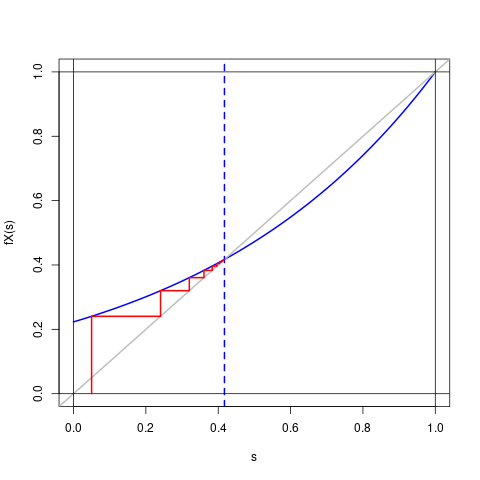
\includegraphics[width=.4\textwidth, trim=0 10 25 50, clip=]{GaltonWatson-fixPoint-q05}
  \end{tabular}
  &
  \begin{tabular}{cc}
  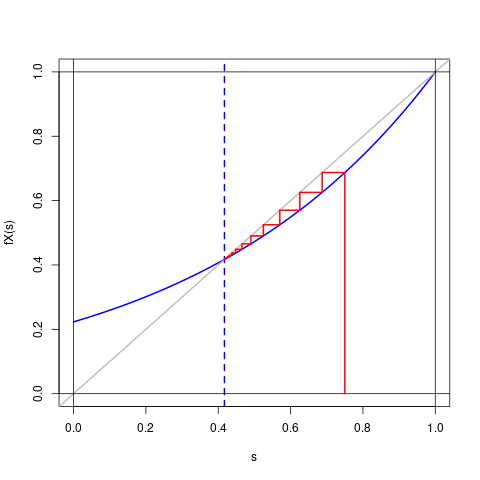
\includegraphics[width=.4\textwidth, trim=0 10 25 50, clip=]{GaltonWatson-fixPoint-q075}
  \end{tabular}
\end{tabular}
$$
\eproof

\remarks
\begin{enumerate}
  \item\todo{$q_n$ est croissante par construction, la trajectoire partant de $q_0 > s^*$ est donc impossible.}
  \item La convergence est donc démontrée pour $Z_0$ aléatoire, avec $q_0 = \Pr\{Z_0 = 0\} \in [0, 1)$ quelconque. Le cas $Z_0 = 1$ correspond au cas $q_0 = 0$.
  \item La convergence vers le point fixe $s^*$ peut également s'obtenir en montrant qu'il est contractant, c'est-à-dire que $|f'_X(s^*)| < 1$. Pour cela, on rapelle d'abord que $0 < f'_X(0) < 1$ et que $m = f'_x(1) > 1$. En appliquant le théorème des valeurs intermédiaire à $f'_X$, on conclue qu'il existe $\widetilde{s} \in (s^*, 1)$ tel que $f'_X(\widetilde{s}) = 1$. Comme enfin $f_X$ est strictement convexe, $f'_X(s)$ est strictement monotone croissante et donc $0 < f'_X(0) < f'_X(s^*) < f'_X(\widetilde{s}) = 1$.
\end{enumerate}



\newpage %-------------------------------------------------------------------------------
%-------------------------------------------------------------------------------
\section{Processus de Poisson} \label{sec:Proba-Poisson}
%-------------------------------------------------------------------------------

Processus de Poisson et de Poisson ponctuel.

\todo{Voir poly A. Guyader Guy06-ProcMakovSauts}


%-------------------------------------------------------------------------------
\bibliography{/home/robin/Biblio/BibGene}
\bibliographystyle{plainnat}
%-------------------------------------------------------------------------------
%-------------------------------------------------------------------------------
\end{document}
%-------------------------------------------------------------------------------
%-------------------------------------------------------------------------------


